\documentclass{article}
\usepackage{tikz}
\usepackage{siunitx}
\usepackage{float}

\usetikzlibrary{arrows,shapes}
\usepackage{xifthen}

%\usetikzlibrary{external}
%\tikzexternalize[prefix=figures/]

\begin{document}

\section{Basic plots}
\label{sec:basic}

\begin{figure}[H]
  \centering
  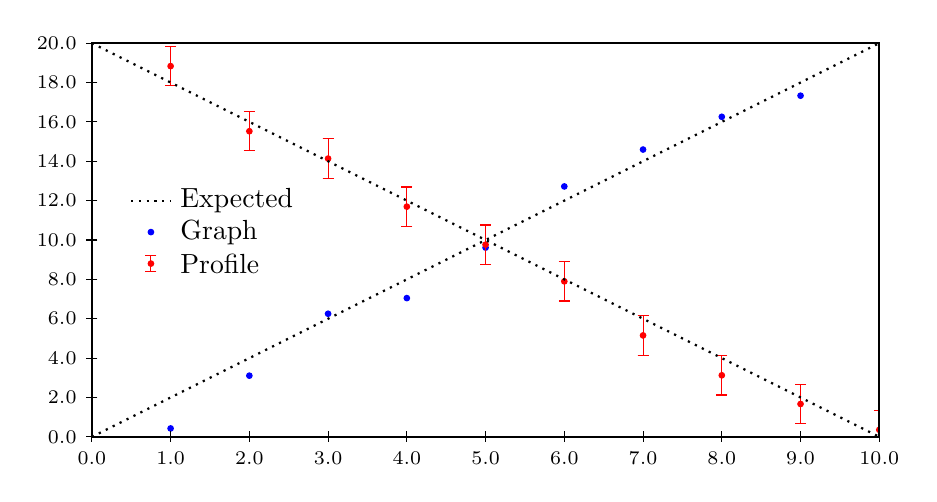
\begin{tikzpicture}
\begin{scope}[]
\clip (0,0) rectangle (10,5);
\draw[blue,fill=blue] (0.0,-0.11265896280989846) circle(1pt); 
\draw[blue,fill=blue] (1.0,0.1067177852637789) circle(1pt); 
\draw[blue,fill=blue] (2.0,0.7769855849859401) circle(1pt); 
\draw[blue,fill=blue] (3.0,1.563221741876979) circle(1pt); 
\draw[blue,fill=blue] (4.0,1.7617895415264044) circle(1pt); 
\draw[blue,fill=blue] (5.0,2.4034006696545265) circle(1pt); 
\draw[blue,fill=blue] (6.0,3.180089516667903) circle(1pt); 
\draw[blue,fill=blue] (7.0,3.648625789175461) circle(1pt); 
\draw[blue,fill=blue] (8.0,4.064206053390634) circle(1pt); 
\draw[blue,fill=blue] (9.0,4.332624590366722) circle(1pt); 
\draw[blue,fill=blue] (10.0,5.326777041467101) circle(1pt); 
\draw[draw=red,fill=red] (0.0,5.124148935749544) -- (0.0,5.624148935749544);
\draw[draw=red,fill=red] (0.0,5.374148935749544) circle(1pt); 
\draw[draw=red,fill=red] (0.0cm -2pt,5.124148935749544) -- (0.0cm + 2pt,5.124148935749544);
\draw[draw=red,fill=red] (0.0cm -2pt,5.624148935749544) -- (0.0cm + 2pt,5.624148935749544);
\draw[draw=red,fill=red] (1.0,4.457987941424418) -- (1.0,4.957987941424418);
\draw[draw=red,fill=red] (1.0,4.707987941424418) circle(1pt); 
\draw[draw=red,fill=red] (1.0cm -2pt,4.457987941424418) -- (1.0cm + 2pt,4.457987941424418);
\draw[draw=red,fill=red] (1.0cm -2pt,4.957987941424418) -- (1.0cm + 2pt,4.957987941424418);
\draw[draw=red,fill=red] (2.0,3.6309822345258023) -- (2.0,4.130982234525803);
\draw[draw=red,fill=red] (2.0,3.8809822345258023) circle(1pt); 
\draw[draw=red,fill=red] (2.0cm -2pt,3.6309822345258023) -- (2.0cm + 2pt,3.6309822345258023);
\draw[draw=red,fill=red] (2.0cm -2pt,4.130982234525803) -- (2.0cm + 2pt,4.130982234525803);
\draw[draw=red,fill=red] (3.0,3.283897225802921) -- (3.0,3.783897225802921);
\draw[draw=red,fill=red] (3.0,3.533897225802921) circle(1pt); 
\draw[draw=red,fill=red] (3.0cm -2pt,3.283897225802921) -- (3.0cm + 2pt,3.283897225802921);
\draw[draw=red,fill=red] (3.0cm -2pt,3.783897225802921) -- (3.0cm + 2pt,3.783897225802921);
\draw[draw=red,fill=red] (4.0,2.6732150073423946) -- (4.0,3.1732150073423946);
\draw[draw=red,fill=red] (4.0,2.9232150073423946) circle(1pt); 
\draw[draw=red,fill=red] (4.0cm -2pt,2.6732150073423946) -- (4.0cm + 2pt,2.6732150073423946);
\draw[draw=red,fill=red] (4.0cm -2pt,3.1732150073423946) -- (4.0cm + 2pt,3.1732150073423946);
\draw[draw=red,fill=red] (5.0,2.190451555285626) -- (5.0,2.690451555285626);
\draw[draw=red,fill=red] (5.0,2.440451555285626) circle(1pt); 
\draw[draw=red,fill=red] (5.0cm -2pt,2.190451555285626) -- (5.0cm + 2pt,2.190451555285626);
\draw[draw=red,fill=red] (5.0cm -2pt,2.690451555285626) -- (5.0cm + 2pt,2.690451555285626);
\draw[draw=red,fill=red] (6.0,1.7244627675920052) -- (6.0,2.224462767592005);
\draw[draw=red,fill=red] (6.0,1.9744627675920052) circle(1pt); 
\draw[draw=red,fill=red] (6.0cm -2pt,1.7244627675920052) -- (6.0cm + 2pt,1.7244627675920052);
\draw[draw=red,fill=red] (6.0cm -2pt,2.224462767592005) -- (6.0cm + 2pt,2.224462767592005);
\draw[draw=red,fill=red] (7.0,1.0380715044115072) -- (7.0,1.5380715044115072);
\draw[draw=red,fill=red] (7.0,1.2880715044115072) circle(1pt); 
\draw[draw=red,fill=red] (7.0cm -2pt,1.0380715044115072) -- (7.0cm + 2pt,1.0380715044115072);
\draw[draw=red,fill=red] (7.0cm -2pt,1.5380715044115072) -- (7.0cm + 2pt,1.5380715044115072);
\draw[draw=red,fill=red] (8.0,0.5317291768813934) -- (8.0,1.0317291768813934);
\draw[draw=red,fill=red] (8.0,0.7817291768813934) circle(1pt); 
\draw[draw=red,fill=red] (8.0cm -2pt,0.5317291768813934) -- (8.0cm + 2pt,0.5317291768813934);
\draw[draw=red,fill=red] (8.0cm -2pt,1.0317291768813934) -- (8.0cm + 2pt,1.0317291768813934);
\draw[draw=red,fill=red] (9.0,0.16715869395498462) -- (9.0,0.6671586939549846);
\draw[draw=red,fill=red] (9.0,0.4171586939549846) circle(1pt); 
\draw[draw=red,fill=red] (9.0cm -2pt,0.16715869395498462) -- (9.0cm + 2pt,0.16715869395498462);
\draw[draw=red,fill=red] (9.0cm -2pt,0.6671586939549846) -- (9.0cm + 2pt,0.6671586939549846);
\draw[draw=red,fill=red] (10.0,-0.16059765768477846) -- (10.0,0.33940234231522154);
\draw[draw=red,fill=red] (10.0,0.08940234231522154) circle(1pt); 
\draw[draw=red,fill=red] (10.0cm -2pt,-0.16059765768477846) -- (10.0cm + 2pt,-0.16059765768477846);
\draw[draw=red,fill=red] (10.0cm -2pt,0.33940234231522154) -- (10.0cm + 2pt,0.33940234231522154);
\draw[thick,dotted] (0.5,3.0) -- (1.0,3.0);
\node[right,] at (1.0,3.0) {Expected};
\draw[blue,fill=blue] (0.75,2.6) circle(1pt); 
\node[right,] at (1.0,2.6) {Graph};
\draw[red, fill=red] (0.75,2.1000001) -- (0.75,2.3);
\draw[red, fill=red] (0.75,2.2) circle(1pt); 
\draw[red, fill=red] (0.75cm -2pt,2.1000001) -- (0.75cm + 2pt,2.1000001);
\draw[red, fill=red] (0.75cm -2pt,2.3) -- (0.75cm + 2pt,2.3);
\node[right,] at (1.0,2.2) {Profile};
\end{scope}
\draw (0,0cm + 2pt) -- (0, 0cm -2pt) node[below] {\scriptsize{\num[round-mode=places,round-precision=1]{0}}};
\draw (1,0cm + 2pt) -- (1, 0cm -2pt) node[below] {\scriptsize{\num[round-mode=places,round-precision=1]{1}}};
\draw (2,0cm + 2pt) -- (2, 0cm -2pt) node[below] {\scriptsize{\num[round-mode=places,round-precision=1]{2}}};
\draw (3,0cm + 2pt) -- (3, 0cm -2pt) node[below] {\scriptsize{\num[round-mode=places,round-precision=1]{3}}};
\draw (4,0cm + 2pt) -- (4, 0cm -2pt) node[below] {\scriptsize{\num[round-mode=places,round-precision=1]{4}}};
\draw (5,0cm + 2pt) -- (5, 0cm -2pt) node[below] {\scriptsize{\num[round-mode=places,round-precision=1]{5}}};
\draw (6,0cm + 2pt) -- (6, 0cm -2pt) node[below] {\scriptsize{\num[round-mode=places,round-precision=1]{6}}};
\draw (7,0cm + 2pt) -- (7, 0cm -2pt) node[below] {\scriptsize{\num[round-mode=places,round-precision=1]{7}}};
\draw (8,0cm + 2pt) -- (8, 0cm -2pt) node[below] {\scriptsize{\num[round-mode=places,round-precision=1]{8}}};
\draw (9,0cm + 2pt) -- (9, 0cm -2pt) node[below] {\scriptsize{\num[round-mode=places,round-precision=1]{9}}};
\draw (10,0cm + 2pt) -- (10, 0cm -2pt) node[below] {\scriptsize{\num[round-mode=places,round-precision=1]{10}}};
\draw (0cm + 2pt,0.    ) -- (0cm-2pt,0.    ) node[left] {\scriptsize{\num[round-mode=places,round-precision=1]{0}}};
\draw (0cm + 2pt,0.5    ) -- (0cm-2pt,0.5    ) node[left] {\scriptsize{\num[round-mode=places,round-precision=1]{2}}};
\draw (0cm + 2pt,1.    ) -- (0cm-2pt,1.    ) node[left] {\scriptsize{\num[round-mode=places,round-precision=1]{4}}};
\draw (0cm + 2pt,1.5    ) -- (0cm-2pt,1.5    ) node[left] {\scriptsize{\num[round-mode=places,round-precision=1]{6}}};
\draw (0cm + 2pt,2.    ) -- (0cm-2pt,2.    ) node[left] {\scriptsize{\num[round-mode=places,round-precision=1]{8}}};
\draw (0cm + 2pt,2.5    ) -- (0cm-2pt,2.5    ) node[left] {\scriptsize{\num[round-mode=places,round-precision=1]{10}}};
\draw (0cm + 2pt,3.    ) -- (0cm-2pt,3.    ) node[left] {\scriptsize{\num[round-mode=places,round-precision=1]{12}}};
\draw (0cm + 2pt,3.5    ) -- (0cm-2pt,3.5    ) node[left] {\scriptsize{\num[round-mode=places,round-precision=1]{14}}};
\draw (0cm + 2pt,4.    ) -- (0cm-2pt,4.    ) node[left] {\scriptsize{\num[round-mode=places,round-precision=1]{16}}};
\draw (0cm + 2pt,4.5    ) -- (0cm-2pt,4.5    ) node[left] {\scriptsize{\num[round-mode=places,round-precision=1]{18}}};
\draw (0cm + 2pt,5.    ) -- (0cm-2pt,5.    ) node[left] {\scriptsize{\num[round-mode=places,round-precision=1]{20}}};
\draw[thick,dotted] (0.0,0.0) -- (10.0,5.0);
\draw[thick,dotted] (0.0,5.0) -- (10.0,0.0);
\draw[thick] (0,0) rectangle (10,5);
\end{tikzpicture}
%%% Local Variables: 
%%% mode: latex 
%%% TeX-master: "master" 
%%% End:


  \caption{Data points with and without errors}
\end{figure}

\begin{figure}[H]
  \centering
  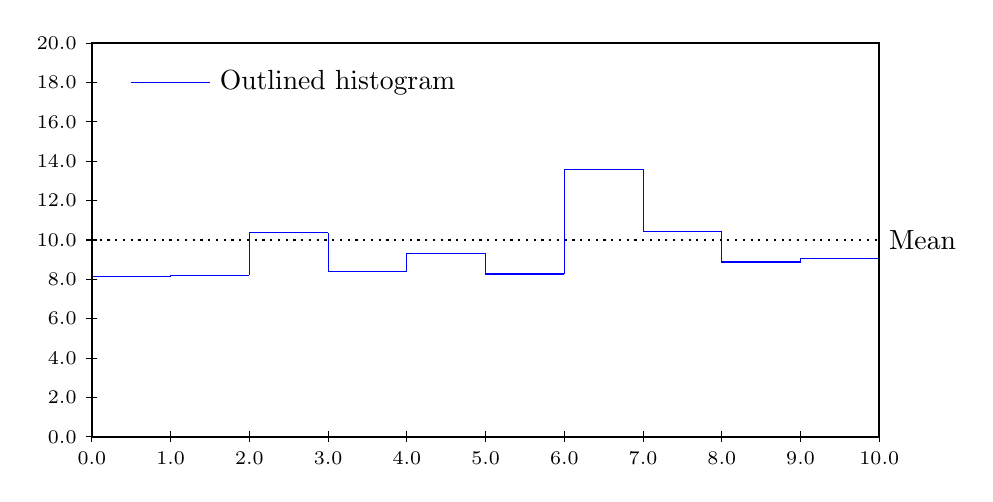
\begin{tikzpicture}
\begin{scope}[]
\clip (0,0) rectangle (10,5);
\begin{scope}[blue]
\draw[] (0.0,2.040753989729346) -- (1.0,2.040753989729346);
\draw (1.0,2.040753989729346) -- (1.0,2.0520371396851527) -- (2.0,2.0520371396851527);
\draw (2.0,2.0520371396851527) -- (2.0,2.589490136587087) -- (3.0,2.589490136587087);
\draw (3.0,2.589490136587087) -- (3.0,2.10531930397396) -- (4.0,2.10531930397396);
\draw (4.0,2.10531930397396) -- (4.0,2.328047479221825) -- (5.0,2.328047479221825);
\draw (5.0,2.328047479221825) -- (5.0,2.067390163042384) -- (6.0,2.067390163042384);
\draw (6.0,2.067390163042384) -- (6.0,3.3961419895360887) -- (7.0,3.3961419895360887);
\draw (7.0,3.3961419895360887) -- (7.0,2.6085288458106475) -- (8.0,2.6085288458106475);
\draw (8.0,2.6085288458106475) -- (8.0,2.2210174657245827) -- (9.0,2.2210174657245827);
\draw (9.0,2.2210174657245827) -- (9.0,2.2670683657782047) -- (10.0,2.2670683657782047);
\end{scope}
\end{scope}
\draw (0,0cm + 2pt) -- (0, 0cm -2pt) node[below] {\scriptsize{\num[round-mode=places,round-precision=1]{0}}};
\draw (1,0cm + 2pt) -- (1, 0cm -2pt) node[below] {\scriptsize{\num[round-mode=places,round-precision=1]{1}}};
\draw (2,0cm + 2pt) -- (2, 0cm -2pt) node[below] {\scriptsize{\num[round-mode=places,round-precision=1]{2}}};
\draw (3,0cm + 2pt) -- (3, 0cm -2pt) node[below] {\scriptsize{\num[round-mode=places,round-precision=1]{3}}};
\draw (4,0cm + 2pt) -- (4, 0cm -2pt) node[below] {\scriptsize{\num[round-mode=places,round-precision=1]{4}}};
\draw (5,0cm + 2pt) -- (5, 0cm -2pt) node[below] {\scriptsize{\num[round-mode=places,round-precision=1]{5}}};
\draw (6,0cm + 2pt) -- (6, 0cm -2pt) node[below] {\scriptsize{\num[round-mode=places,round-precision=1]{6}}};
\draw (7,0cm + 2pt) -- (7, 0cm -2pt) node[below] {\scriptsize{\num[round-mode=places,round-precision=1]{7}}};
\draw (8,0cm + 2pt) -- (8, 0cm -2pt) node[below] {\scriptsize{\num[round-mode=places,round-precision=1]{8}}};
\draw (9,0cm + 2pt) -- (9, 0cm -2pt) node[below] {\scriptsize{\num[round-mode=places,round-precision=1]{9}}};
\draw (10,0cm + 2pt) -- (10, 0cm -2pt) node[below] {\scriptsize{\num[round-mode=places,round-precision=1]{10}}};
\draw (0cm + 2pt,0.    ) -- (0cm-2pt,0.    ) node[left] {\scriptsize{\num[round-mode=places,round-precision=1]{0}}};
\draw (0cm + 2pt,0.5    ) -- (0cm-2pt,0.5    ) node[left] {\scriptsize{\num[round-mode=places,round-precision=1]{2}}};
\draw (0cm + 2pt,1.    ) -- (0cm-2pt,1.    ) node[left] {\scriptsize{\num[round-mode=places,round-precision=1]{4}}};
\draw (0cm + 2pt,1.5    ) -- (0cm-2pt,1.5    ) node[left] {\scriptsize{\num[round-mode=places,round-precision=1]{6}}};
\draw (0cm + 2pt,2.    ) -- (0cm-2pt,2.    ) node[left] {\scriptsize{\num[round-mode=places,round-precision=1]{8}}};
\draw (0cm + 2pt,2.5    ) -- (0cm-2pt,2.5    ) node[left] {\scriptsize{\num[round-mode=places,round-precision=1]{10}}};
\draw (0cm + 2pt,3.    ) -- (0cm-2pt,3.    ) node[left] {\scriptsize{\num[round-mode=places,round-precision=1]{12}}};
\draw (0cm + 2pt,3.5    ) -- (0cm-2pt,3.5    ) node[left] {\scriptsize{\num[round-mode=places,round-precision=1]{14}}};
\draw (0cm + 2pt,4.    ) -- (0cm-2pt,4.    ) node[left] {\scriptsize{\num[round-mode=places,round-precision=1]{16}}};
\draw (0cm + 2pt,4.5    ) -- (0cm-2pt,4.5    ) node[left] {\scriptsize{\num[round-mode=places,round-precision=1]{18}}};
\draw (0cm + 2pt,5.    ) -- (0cm-2pt,5.    ) node[left] {\scriptsize{\num[round-mode=places,round-precision=1]{20}}};
\draw[thick] (0,0) rectangle (10,5);
\draw[thick,dotted] (0.0,2.5) -- (10.0,2.5);
\node[right] at (10.0,2.5) {Mean};
\draw[blue] (0.5,4.5) -- (1.5,4.5);
\node[right,] at (1.5,4.5) {Outlined histogram};
\end{tikzpicture}
%%% Local Variables: 
%%% mode: latex 
%%% TeX-master: "master" 
%%% End:


  \caption{Basic histogram}
\end{figure}

\begin{figure}[H]
  \centering
  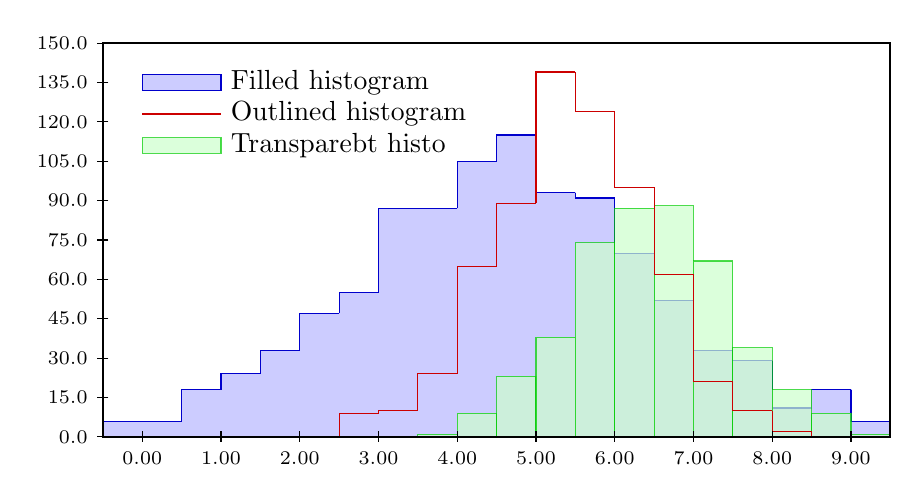
\begin{tikzpicture}
\begin{scope}[]
\clip (0,0) rectangle (10,5);
\begin{scope}[draw=blue!20,fill=blue!20]
\filldraw[] (0.0,0.0) -- (0.0,0.2) -- (0.5,0.2) -- (0.5,0.0);
\filldraw[] (0.5,0.0) -- (0.5,0.2) -- (1.0,0.2) -- (1.0,0.0);
\filldraw[] (1.0,0.0) -- (1.0,0.6) -- (1.5,0.6) -- (1.5,0.0);
\filldraw[] (1.5,0.0) -- (1.5,0.8) -- (2.0,0.8) -- (2.0,0.0);
\filldraw[] (2.0,0.0) -- (2.0,1.1) -- (2.5,1.1) -- (2.5,0.0);
\filldraw[] (2.5,0.0) -- (2.5,1.5666667) -- (3.0,1.5666667) -- (3.0,0.0);
\filldraw[] (3.0,0.0) -- (3.0,1.8333334) -- (3.5,1.8333334) -- (3.5,0.0);
\filldraw[] (3.5,0.0) -- (3.5,2.9) -- (4.0,2.9) -- (4.0,0.0);
\filldraw[] (4.0,0.0) -- (4.0,2.9) -- (4.5,2.9) -- (4.5,0.0);
\filldraw[] (4.5,0.0) -- (4.5,3.5) -- (5.0,3.5) -- (5.0,0.0);
\filldraw[] (5.0,0.0) -- (5.0,3.8333333) -- (5.5,3.8333333) -- (5.5,0.0);
\filldraw[] (5.5,0.0) -- (5.5,3.1) -- (6.0,3.1) -- (6.0,0.0);
\filldraw[] (6.0,0.0) -- (6.0,3.0333333) -- (6.5,3.0333333) -- (6.5,0.0);
\filldraw[] (6.5,0.0) -- (6.5,2.3333333) -- (7.0,2.3333333) -- (7.0,0.0);
\filldraw[] (7.0,0.0) -- (7.0,1.7333333) -- (7.5,1.7333333) -- (7.5,0.0);
\filldraw[] (7.5,0.0) -- (7.5,1.1) -- (8.0,1.1) -- (8.0,0.0);
\filldraw[] (8.0,0.0) -- (8.0,0.96666664) -- (8.5,0.96666664) -- (8.5,0.0);
\filldraw[] (8.5,0.0) -- (8.5,0.36666667) -- (9.0,0.36666667) -- (9.0,0.0);
\filldraw[] (9.0,0.0) -- (9.0,0.6) -- (9.5,0.6) -- (9.5,0.0);
\filldraw[] (9.5,0.0) -- (9.5,0.2) -- (10.0,0.2) -- (10.0,0.0);
\end{scope}
\begin{scope}[blue!80!black]
\draw[] (0.0,0.2) -- (0.5,0.2);
\draw (0.5,0.2) -- (0.5,0.2) -- (1.0,0.2);
\draw (1.0,0.2) -- (1.0,0.6) -- (1.5,0.6);
\draw (1.5,0.6) -- (1.5,0.8) -- (2.0,0.8);
\draw (2.0,0.8) -- (2.0,1.1) -- (2.5,1.1);
\draw (2.5,1.1) -- (2.5,1.5666667) -- (3.0,1.5666667);
\draw (3.0,1.5666667) -- (3.0,1.8333334) -- (3.5,1.8333334);
\draw (3.5,1.8333334) -- (3.5,2.9) -- (4.0,2.9);
\draw (4.0,2.9) -- (4.0,2.9) -- (4.5,2.9);
\draw (4.5,2.9) -- (4.5,3.5) -- (5.0,3.5);
\draw (5.0,3.5) -- (5.0,3.8333333) -- (5.5,3.8333333);
\draw (5.5,3.8333333) -- (5.5,3.1) -- (6.0,3.1);
\draw (6.0,3.1) -- (6.0,3.0333333) -- (6.5,3.0333333);
\draw (6.5,3.0333333) -- (6.5,2.3333333) -- (7.0,2.3333333);
\draw (7.0,2.3333333) -- (7.0,1.7333333) -- (7.5,1.7333333);
\draw (7.5,1.7333333) -- (7.5,1.1) -- (8.0,1.1);
\draw (8.0,1.1) -- (8.0,0.96666664) -- (8.5,0.96666664);
\draw (8.5,0.96666664) -- (8.5,0.36666667) -- (9.0,0.36666667);
\draw (9.0,0.36666667) -- (9.0,0.6) -- (9.5,0.6);
\draw (9.5,0.6) -- (9.5,0.2) -- (10.0,0.2);
\end{scope}
\begin{scope}[opacity=0.7,draw=green!80!black,fill=green!20]
\filldraw[] (0.0,0.0) -- (0.0,0.0) -- (0.5,0.0) -- (0.5,0.0);
\filldraw[] (0.5,0.0) -- (0.5,0.0) -- (1.0,0.0) -- (1.0,0.0);
\filldraw[] (1.0,0.0) -- (1.0,0.0) -- (1.5,0.0) -- (1.5,0.0);
\filldraw[] (1.5,0.0) -- (1.5,0.0) -- (2.0,0.0) -- (2.0,0.0);
\filldraw[] (2.0,0.0) -- (2.0,0.0) -- (2.5,0.0) -- (2.5,0.0);
\filldraw[] (2.5,0.0) -- (2.5,0.0) -- (3.0,0.0) -- (3.0,0.0);
\filldraw[] (3.0,0.0) -- (3.0,0.0) -- (3.5,0.0) -- (3.5,0.0);
\filldraw[] (3.5,0.0) -- (3.5,0.0) -- (4.0,0.0) -- (4.0,0.0);
\filldraw[] (4.0,0.0) -- (4.0,0.033333335) -- (4.5,0.033333335) -- (4.5,0.0);
\filldraw[] (4.5,0.0) -- (4.5,0.3) -- (5.0,0.3) -- (5.0,0.0);
\filldraw[] (5.0,0.0) -- (5.0,0.76666665) -- (5.5,0.76666665) -- (5.5,0.0);
\filldraw[] (5.5,0.0) -- (5.5,1.2666667) -- (6.0,1.2666667) -- (6.0,0.0);
\filldraw[] (6.0,0.0) -- (6.0,2.4666667) -- (6.5,2.4666667) -- (6.5,0.0);
\filldraw[] (6.5,0.0) -- (6.5,2.9) -- (7.0,2.9) -- (7.0,0.0);
\filldraw[] (7.0,0.0) -- (7.0,2.9333334) -- (7.5,2.9333334) -- (7.5,0.0);
\filldraw[] (7.5,0.0) -- (7.5,2.2333333) -- (8.0,2.2333333) -- (8.0,0.0);
\filldraw[] (8.0,0.0) -- (8.0,1.1333333) -- (8.5,1.1333333) -- (8.5,0.0);
\filldraw[] (8.5,0.0) -- (8.5,0.6) -- (9.0,0.6) -- (9.0,0.0);
\filldraw[] (9.0,0.0) -- (9.0,0.3) -- (9.5,0.3) -- (9.5,0.0);
\filldraw[] (9.5,0.0) -- (9.5,0.033333335) -- (10.0,0.033333335) -- (10.0,0.0);
\end{scope}
\begin{scope}[red!80!black]
\draw[] (0.0,0.0) -- (0.5,0.0);
\draw (0.5,0.0) -- (0.5,0.0) -- (1.0,0.0);
\draw (1.0,0.0) -- (1.0,0.0) -- (1.5,0.0);
\draw (1.5,0.0) -- (1.5,0.0) -- (2.0,0.0);
\draw (2.0,0.0) -- (2.0,0.0) -- (2.5,0.0);
\draw (2.5,0.0) -- (2.5,0.0) -- (3.0,0.0);
\draw (3.0,0.0) -- (3.0,0.3) -- (3.5,0.3);
\draw (3.5,0.3) -- (3.5,0.33333334) -- (4.0,0.33333334);
\draw (4.0,0.33333334) -- (4.0,0.8) -- (4.5,0.8);
\draw (4.5,0.8) -- (4.5,2.1666667) -- (5.0,2.1666667);
\draw (5.0,2.1666667) -- (5.0,2.9666667) -- (5.5,2.9666667);
\draw (5.5,2.9666667) -- (5.5,4.633333) -- (6.0,4.633333);
\draw (6.0,4.633333) -- (6.0,4.133333) -- (6.5,4.133333);
\draw (6.5,4.133333) -- (6.5,3.1666667) -- (7.0,3.1666667);
\draw (7.0,3.1666667) -- (7.0,2.0666666) -- (7.5,2.0666666);
\draw (7.5,2.0666666) -- (7.5,0.7) -- (8.0,0.7);
\draw (8.0,0.7) -- (8.0,0.33333334) -- (8.5,0.33333334);
\draw (8.5,0.33333334) -- (8.5,0.06666667) -- (9.0,0.06666667);
\draw (9.0,0.06666667) -- (9.0,0.0) -- (9.5,0.0);
\draw (9.5,0.0) -- (9.5,0.0) -- (10.0,0.0);
\end{scope}
\end{scope}
\draw (0.5,0cm + 2pt) -- (0.5, 0cm -2pt) node[below] {\scriptsize{\num[round-mode=places,round-precision=2]{0}}};
\draw (1.5,0cm + 2pt) -- (1.5, 0cm -2pt) node[below] {\scriptsize{\num[round-mode=places,round-precision=2]{1}}};
\draw (2.5,0cm + 2pt) -- (2.5, 0cm -2pt) node[below] {\scriptsize{\num[round-mode=places,round-precision=2]{2}}};
\draw (3.5,0cm + 2pt) -- (3.5, 0cm -2pt) node[below] {\scriptsize{\num[round-mode=places,round-precision=2]{3}}};
\draw (4.5,0cm + 2pt) -- (4.5, 0cm -2pt) node[below] {\scriptsize{\num[round-mode=places,round-precision=2]{4}}};
\draw (5.5,0cm + 2pt) -- (5.5, 0cm -2pt) node[below] {\scriptsize{\num[round-mode=places,round-precision=2]{5}}};
\draw (6.5,0cm + 2pt) -- (6.5, 0cm -2pt) node[below] {\scriptsize{\num[round-mode=places,round-precision=2]{6}}};
\draw (7.5,0cm + 2pt) -- (7.5, 0cm -2pt) node[below] {\scriptsize{\num[round-mode=places,round-precision=2]{7}}};
\draw (8.5,0cm + 2pt) -- (8.5, 0cm -2pt) node[below] {\scriptsize{\num[round-mode=places,round-precision=2]{8}}};
\draw (9.5,0cm + 2pt) -- (9.5, 0cm -2pt) node[below] {\scriptsize{\num[round-mode=places,round-precision=2]{9}}};
\draw (0cm + 2pt,0.    ) -- (0cm-2pt,0.    ) node[left] {\scriptsize{\num[round-mode=places,round-precision=1]{0}}};
\draw (0cm + 2pt,0.5    ) -- (0cm-2pt,0.5    ) node[left] {\scriptsize{\num[round-mode=places,round-precision=1]{15}}};
\draw (0cm + 2pt,1.    ) -- (0cm-2pt,1.    ) node[left] {\scriptsize{\num[round-mode=places,round-precision=1]{30}}};
\draw (0cm + 2pt,1.5    ) -- (0cm-2pt,1.5    ) node[left] {\scriptsize{\num[round-mode=places,round-precision=1]{45}}};
\draw (0cm + 2pt,2.    ) -- (0cm-2pt,2.    ) node[left] {\scriptsize{\num[round-mode=places,round-precision=1]{60}}};
\draw (0cm + 2pt,2.5    ) -- (0cm-2pt,2.5    ) node[left] {\scriptsize{\num[round-mode=places,round-precision=1]{75}}};
\draw (0cm + 2pt,3.    ) -- (0cm-2pt,3.    ) node[left] {\scriptsize{\num[round-mode=places,round-precision=1]{90}}};
\draw (0cm + 2pt,3.5    ) -- (0cm-2pt,3.5    ) node[left] {\scriptsize{\num[round-mode=places,round-precision=1]{105}}};
\draw (0cm + 2pt,4.    ) -- (0cm-2pt,4.    ) node[left] {\scriptsize{\num[round-mode=places,round-precision=1]{120}}};
\draw (0cm + 2pt,4.5    ) -- (0cm-2pt,4.5    ) node[left] {\scriptsize{\num[round-mode=places,round-precision=1]{135}}};
\draw (0cm + 2pt,5.    ) -- (0cm-2pt,5.    ) node[left] {\scriptsize{\num[round-mode=places,round-precision=1]{150}}};
\draw[thick] (0,0) rectangle (10,5);
\draw[draw=blue!20,fill=blue!20] (0.5,4.4) rectangle (1.5,4.6);
; 
\draw[blue!80!black] (0.5,4.4) rectangle (1.5,4.6);
; 
\node[right,] at (1.5,4.5) {Filled histogram};
\draw[red!80!black] (0.5,4.1) -- (1.5,4.1);
\node[right,] at (1.5,4.1) {Outlined histogram};
\draw[opacity=0.7,draw=green!80!black,fill=green!20] (0.5,3.6000001) rectangle (1.5,3.8);
; 
\node[right,] at (1.5,3.7) {Transparebt histo};
\end{tikzpicture}
%%% Local Variables: 
%%% mode: latex 
%%% TeX-master: "master" 
%%% End:


  \caption{Three histograms in the same figure}
\end{figure}

\section{Fitting with Levenberg marquart algorithm and splines}
\label{sec:LMA}

\begin{figure}[H]
  \centering
  %%% AUTO GENERATED CODE
\documentclass{standalone}
\ifx\HCode\UnDef\else\def\pgfsysdriver{pgfsys-tex4ht.def}\fi
\usepackage[usenames,dvipsnames,svgnames,table]{xcolor}
\usepackage[utf8]{inputenc}
\usepackage[]{textcomp}
\usepackage{tikz}
\usepackage{color}
\usepackage{siunitx}
\usetikzlibrary{arrows,shapes}
\usetikzlibrary{decorations.markings}
\begin{document}
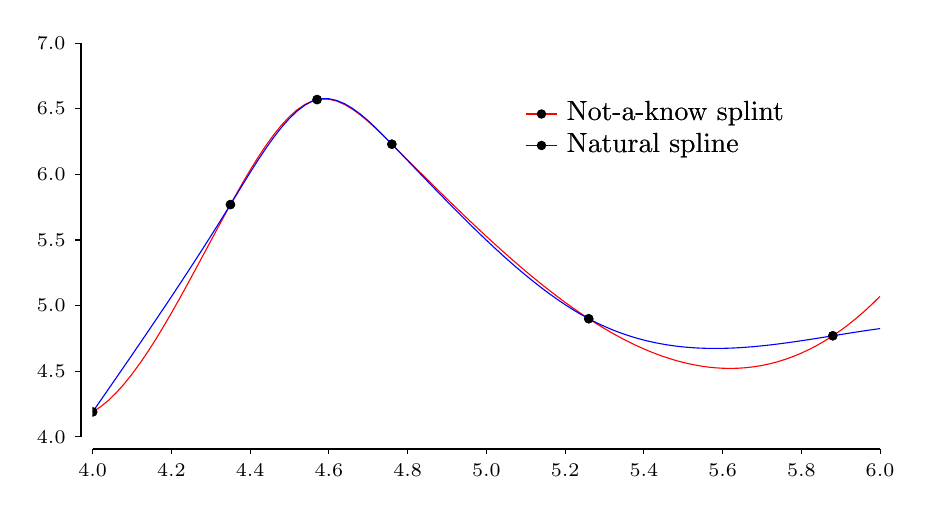
\begin{tikzpicture}[]
\begin{scope}[]
\pgfpathmoveto{ \pgfpointadd{\pgfpointxy {0.0} {0.0}} {\pgfpoint{0cm}{0cm}} }
\pgfpathlineto{ \pgfpointadd{\pgfpointxy {0.0} {0.0}} {\pgfpoint{10cm}{0cm}} }
\pgfpathlineto{ \pgfpointadd{\pgfpointxy {0.0} {0.0}} {\pgfpoint{10cm}{5cm}} }
\pgfpathlineto{ \pgfpointadd{\pgfpointxy {0.0} {0.0}} {\pgfpoint{0cm}{5cm}} }
\pgfpathclose
\pgfusepath{  clip, }
\begin{scope}[shift={(0.0,0.0)}]
\pgfsetxvec{\pgfpoint{5.0cm}{0cm}}
\pgfsetyvec{\pgfpoint{0cm}{1.6666666666666667cm}}
\begin{scope}[shift={(-4.0,-4.0)}]
\begin{scope}[]
\pgfpathmoveto{ \pgfpointadd{\pgfpointxy {4.0} {4.0}} {\pgfpoint{0cm}{0cm}} }
\pgfpathlineto{ \pgfpointadd{\pgfpointxy {4.0} {4.0}} {\pgfpoint{10cm}{0cm}} }
\pgfpathlineto{ \pgfpointadd{\pgfpointxy {4.0} {4.0}} {\pgfpoint{10cm}{5cm}} }
\pgfpathlineto{ \pgfpointadd{\pgfpointxy {4.0} {4.0}} {\pgfpoint{0cm}{5cm}} }
\pgfpathclose
\pgfusepath{  clip, }
\begin{scope}[red]
\pgfpathmoveto{ \pgfpointxy {4.0} {4.19}}
\pgfpathlineto{ \pgfpointxy {4.02} {4.2288933173496535}}
\pgfpathlineto{ \pgfpointxy {4.04} {4.277870024848159}}
\pgfpathlineto{ \pgfpointxy {4.06} {4.336184185327374}}
\pgfpathlineto{ \pgfpointxy {4.08} {4.403089861619165}}
\pgfpathlineto{ \pgfpointxy {4.1} {4.477841116555382}}
\pgfpathlineto{ \pgfpointxy {4.12} {4.559692012967896}}
\pgfpathlineto{ \pgfpointxy {4.14} {4.647896613688557}}
\pgfpathlineto{ \pgfpointxy {4.16} {4.741708981549234}}
\pgfpathlineto{ \pgfpointxy {4.18} {4.84038317938178}}
\pgfpathlineto{ \pgfpointxy {4.2} {4.943173270018062}}
\pgfpathlineto{ \pgfpointxy {4.22} {5.049333316289932}}
\pgfpathlineto{ \pgfpointxy {4.24} {5.158117381029259}}
\pgfpathlineto{ \pgfpointxy {4.26} {5.268779527067894}}
\pgfpathlineto{ \pgfpointxy {4.28} {5.380573817237705}}
\pgfpathlineto{ \pgfpointxy {4.3} {5.492754314370545}}
\pgfpathlineto{ \pgfpointxy {4.32} {5.604575081298282}}
\pgfpathlineto{ \pgfpointxy {4.34} {5.715290180852768}}
\pgfpathlineto{ \pgfpointxy {4.36} {5.824144492927248}}
\pgfpathlineto{ \pgfpointxy {4.38} {5.930171689826624}}
\pgfpathlineto{ \pgfpointxy {4.4} {6.032194236267487}}
\pgfpathlineto{ \pgfpointxy {4.42} {6.129025414027786}}
\pgfpathlineto{ \pgfpointxy {4.44} {6.2194785048854895}}
\pgfpathlineto{ \pgfpointxy {4.46} {6.302366790618549}}
\pgfpathlineto{ \pgfpointxy {4.48} {6.376503553004932}}
\pgfpathlineto{ \pgfpointxy {4.5} {6.440702073822589}}
\pgfpathlineto{ \pgfpointxy {4.52} {6.493775634849485}}
\pgfpathlineto{ \pgfpointxy {4.54} {6.53453751786358}}
\pgfpathlineto{ \pgfpointxy {4.5600000000000005} {6.56180100464283}}
\pgfpathlineto{ \pgfpointxy {4.58} {6.574437556572912}}
\pgfpathlineto{ \pgfpointxy {4.6} {6.572656766016991}}
\pgfpathlineto{ \pgfpointxy {4.62} {6.558006356315717}}
\pgfpathlineto{ \pgfpointxy {4.64} {6.532092230417464}}
\pgfpathlineto{ \pgfpointxy {4.66} {6.496520291270597}}
\pgfpathlineto{ \pgfpointxy {4.68} {6.452896441823487}}
\pgfpathlineto{ \pgfpointxy {4.7} {6.402826585024502}}
\pgfpathlineto{ \pgfpointxy {4.72} {6.347916623822015}}
\pgfpathlineto{ \pgfpointxy {4.74} {6.2897724611643895}}
\pgfpathlineto{ \pgfpointxy {4.76} {6.23}}
\pgfpathlineto{ \pgfpointxy {4.78} {6.169948902792082}}
\pgfpathlineto{ \pgfpointxy {4.8} {6.109943870063351}}
\pgfpathlineto{ \pgfpointxy {4.82} {6.050053361851389}}
\pgfpathlineto{ \pgfpointxy {4.84} {5.990345838193781}}
\pgfpathlineto{ \pgfpointxy {4.86} {5.9308897591281085}}
\pgfpathlineto{ \pgfpointxy {4.88} {5.871753584691959}}
\pgfpathlineto{ \pgfpointxy {4.9} {5.813005774922911}}
\pgfpathlineto{ \pgfpointxy {4.92} {5.754714789858553}}
\pgfpathlineto{ \pgfpointxy {4.94} {5.696949089536464}}
\pgfpathlineto{ \pgfpointxy {4.96} {5.639777133994231}}
\pgfpathlineto{ \pgfpointxy {4.98} {5.583267383269433}}
\pgfpathlineto{ \pgfpointxy {5.0} {5.5274882973996595}}
\pgfpathlineto{ \pgfpointxy {5.02} {5.47250833642249}}
\pgfpathlineto{ \pgfpointxy {5.04} {5.418395960375507}}
\pgfpathlineto{ \pgfpointxy {5.0600000000000005} {5.365219629296296}}
\pgfpathlineto{ \pgfpointxy {5.08} {5.3130478032224415}}
\pgfpathlineto{ \pgfpointxy {5.1} {5.261948942191526}}
\pgfpathlineto{ \pgfpointxy {5.12} {5.21199150624113}}
\pgfpathlineto{ \pgfpointxy {5.140000000000001} {5.1632439554088405}}
\pgfpathlineto{ \pgfpointxy {5.16} {5.115774749732242}}
\pgfpathlineto{ \pgfpointxy {5.18} {5.069652349248916}}
\pgfpathlineto{ \pgfpointxy {5.2} {5.0249452139964434}}
\pgfpathlineto{ \pgfpointxy {5.22} {4.9817218040124125}}
\pgfpathlineto{ \pgfpointxy {5.24} {4.940050579334401}}
\pgfpathlineto{ \pgfpointxy {5.26} {4.9}}
\pgfpathlineto{ \pgfpointxy {5.28} {4.861636317658478}}
\pgfpathlineto{ \pgfpointxy {5.3} {4.8250169504058755}}
\pgfpathlineto{ \pgfpointxy {5.32} {4.790197107949918}}
\pgfpathlineto{ \pgfpointxy {5.34} {4.757231999998338}}
\pgfpathlineto{ \pgfpointxy {5.36} {4.726176836258861}}
\pgfpathlineto{ \pgfpointxy {5.38} {4.697086826439219}}
\pgfpathlineto{ \pgfpointxy {5.4} {4.670017180247137}}
\pgfpathlineto{ \pgfpointxy {5.42} {4.645023107390346}}
\pgfpathlineto{ \pgfpointxy {5.4399999999999995} {4.622159817576572}}
\pgfpathlineto{ \pgfpointxy {5.46} {4.601482520513546}}
\pgfpathlineto{ \pgfpointxy {5.48} {4.583046425908996}}
\pgfpathlineto{ \pgfpointxy {5.5} {4.566906743470651}}
\pgfpathlineto{ \pgfpointxy {5.52} {4.55311868290624}}
\pgfpathlineto{ \pgfpointxy {5.54} {4.5417374539234885}}
\pgfpathlineto{ \pgfpointxy {5.5600000000000005} {4.532818266230128}}
\pgfpathlineto{ \pgfpointxy {5.58} {4.5264163295338875}}
\pgfpathlineto{ \pgfpointxy {5.6} {4.522586853542495}}
\pgfpathlineto{ \pgfpointxy {5.62} {4.521385047963677}}
\pgfpathlineto{ \pgfpointxy {5.640000000000001} {4.522866122505165}}
\pgfpathlineto{ \pgfpointxy {5.66} {4.527085286874686}}
\pgfpathlineto{ \pgfpointxy {5.68} {4.534097750779969}}
\pgfpathlineto{ \pgfpointxy {5.7} {4.543958723928742}}
\pgfpathlineto{ \pgfpointxy {5.72} {4.556723416028735}}
\pgfpathlineto{ \pgfpointxy {5.74} {4.572447036787675}}
\pgfpathlineto{ \pgfpointxy {5.76} {4.591184795913292}}
\pgfpathlineto{ \pgfpointxy {5.78} {4.612991903113314}}
\pgfpathlineto{ \pgfpointxy {5.8} {4.637923568095469}}
\pgfpathlineto{ \pgfpointxy {5.82} {4.666035000567487}}
\pgfpathlineto{ \pgfpointxy {5.84} {4.697381410237095}}
\pgfpathlineto{ \pgfpointxy {5.86} {4.732018006812025}}
\pgfpathlineto{ \pgfpointxy {5.88} {4.77}}
\pgfpathlineto{ \pgfpointxy {5.9} {4.811382599508753}}
\pgfpathlineto{ \pgfpointxy {5.92} {4.85622101504601}}
\pgfpathlineto{ \pgfpointxy {5.9399999999999995} {4.904570456319501}}
\pgfpathlineto{ \pgfpointxy {5.96} {4.9564861330369565}}
\pgfpathlineto{ \pgfpointxy {5.98} {5.0120232549061035}}
\pgfpathlineto{ \pgfpointxy {6.0} {5.071237031634667}}
\pgfusepath{ stroke, }
\end{scope}
\end{scope}
\begin{scope}[]
\pgfpathmoveto{ \pgfpointadd{\pgfpointxy {4.0} {4.0}} {\pgfpoint{0cm}{0cm}} }
\pgfpathlineto{ \pgfpointadd{\pgfpointxy {4.0} {4.0}} {\pgfpoint{10cm}{0cm}} }
\pgfpathlineto{ \pgfpointadd{\pgfpointxy {4.0} {4.0}} {\pgfpoint{10cm}{5cm}} }
\pgfpathlineto{ \pgfpointadd{\pgfpointxy {4.0} {4.0}} {\pgfpoint{0cm}{5cm}} }
\pgfpathclose
\pgfusepath{  clip, }
\node at (4.0,4.19) [fill=black,draw=black,circle,inner sep=0.0pt,minimum width =3.0pt,minimum height=3.0pt] {};
\node at (4.35,5.77) [fill=black,draw=black,circle,inner sep=0.0pt,minimum width =3.0pt,minimum height=3.0pt] {};
\node at (4.57,6.57) [fill=black,draw=black,circle,inner sep=0.0pt,minimum width =3.0pt,minimum height=3.0pt] {};
\node at (4.76,6.23) [fill=black,draw=black,circle,inner sep=0.0pt,minimum width =3.0pt,minimum height=3.0pt] {};
\node at (5.26,4.9) [fill=black,draw=black,circle,inner sep=0.0pt,minimum width =3.0pt,minimum height=3.0pt] {};
\node at (5.88,4.77) [fill=black,draw=black,circle,inner sep=0.0pt,minimum width =3.0pt,minimum height=3.0pt] {};
\end{scope}
\end{scope}
\end{scope}
\pgfsetxvec{\pgfpoint{1cm}{0cm}}
\pgfsetyvec{\pgfpoint{0cm}{1cm}}
\end{scope}
\draw[red] (5.5,4.1) -- (5.9,4.1);
\draw[opacity=0.0,white] (5.5,4.2) -- (5.5,4.0);
\node at (5.9,4.1) [right,] {Not-a-know splint};
\node at (5.7,4.1) [fill=black,draw=black,circle,inner sep=0.0pt,minimum width =3.0pt,minimum height=3.0pt] {};
\node at (5.9,4.1) [right,] {Not-a-know splint};
\begin{scope}[]
\pgfpathmoveto{ \pgfpointadd{\pgfpointxy {0.0} {0.0}} {\pgfpoint{0cm}{0cm}} }
\pgfpathlineto{ \pgfpointadd{\pgfpointxy {0.0} {0.0}} {\pgfpoint{10cm}{0cm}} }
\pgfpathlineto{ \pgfpointadd{\pgfpointxy {0.0} {0.0}} {\pgfpoint{10cm}{5cm}} }
\pgfpathlineto{ \pgfpointadd{\pgfpointxy {0.0} {0.0}} {\pgfpoint{0cm}{5cm}} }
\pgfpathclose
\pgfusepath{  clip, }
\begin{scope}[shift={(0.0,0.0)}]
\pgfsetxvec{\pgfpoint{5.0cm}{0cm}}
\pgfsetyvec{\pgfpoint{0cm}{1.6666666666666667cm}}
\begin{scope}[shift={(-4.0,-4.0)}]
\begin{scope}[]
\pgfpathmoveto{ \pgfpointadd{\pgfpointxy {4.0} {4.0}} {\pgfpoint{0cm}{0cm}} }
\pgfpathlineto{ \pgfpointadd{\pgfpointxy {4.0} {4.0}} {\pgfpoint{10cm}{0cm}} }
\pgfpathlineto{ \pgfpointadd{\pgfpointxy {4.0} {4.0}} {\pgfpoint{10cm}{5cm}} }
\pgfpathlineto{ \pgfpointadd{\pgfpointxy {4.0} {4.0}} {\pgfpoint{0cm}{5cm}} }
\pgfpathclose
\pgfusepath{  clip, }
\begin{scope}[blue]
\pgfpathmoveto{ \pgfpointxy {4.0} {4.19}}
\pgfpathlineto{ \pgfpointxy {4.02} {4.27659219042123}}
\pgfpathlineto{ \pgfpointxy {4.04} {4.363256980820145}}
\pgfpathlineto{ \pgfpointxy {4.06} {4.450066971174415}}
\pgfpathlineto{ \pgfpointxy {4.08} {4.537094761461732}}
\pgfpathlineto{ \pgfpointxy {4.1} {4.624412951659764}}
\pgfpathlineto{ \pgfpointxy {4.12} {4.712094141746202}}
\pgfpathlineto{ \pgfpointxy {4.14} {4.800210931698716}}
\pgfpathlineto{ \pgfpointxy {4.16} {4.888835921494997}}
\pgfpathlineto{ \pgfpointxy {4.18} {4.978041711112716}}
\pgfpathlineto{ \pgfpointxy {4.2} {5.067900900529561}}
\pgfpathlineto{ \pgfpointxy {4.22} {5.158486089723204}}
\pgfpathlineto{ \pgfpointxy {4.24} {5.249869878671334}}
\pgfpathlineto{ \pgfpointxy {4.26} {5.342124867351624}}
\pgfpathlineto{ \pgfpointxy {4.28} {5.43532365574176}}
\pgfpathlineto{ \pgfpointxy {4.3} {5.529538843819415}}
\pgfpathlineto{ \pgfpointxy {4.32} {5.624843031562279}}
\pgfpathlineto{ \pgfpointxy {4.34} {5.721308818948022}}
\pgfpathlineto{ \pgfpointxy {4.36} {5.818974279573464}}
\pgfpathlineto{ \pgfpointxy {4.38} {5.917083380275411}}
\pgfpathlineto{ \pgfpointxy {4.4} {6.014085981130691}}
\pgfpathlineto{ \pgfpointxy {4.42} {6.108397415835243}}
\pgfpathlineto{ \pgfpointxy {4.44} {6.198433018085027}}
\pgfpathlineto{ \pgfpointxy {4.46} {6.282608121575982}}
\pgfpathlineto{ \pgfpointxy {4.48} {6.359338060004066}}
\pgfpathlineto{ \pgfpointxy {4.5} {6.427038167065223}}
\pgfpathlineto{ \pgfpointxy {4.52} {6.484123776455401}}
\pgfpathlineto{ \pgfpointxy {4.54} {6.529010221870556}}
\pgfpathlineto{ \pgfpointxy {4.5600000000000005} {6.560112837006632}}
\pgfpathlineto{ \pgfpointxy {4.58} {6.575914836921859}}
\pgfpathlineto{ \pgfpointxy {4.6} {6.576460708006886}}
\pgfpathlineto{ \pgfpointxy {4.62} {6.563356207984786}}
\pgfpathlineto{ \pgfpointxy {4.64} {6.538274975940911}}
\pgfpathlineto{ \pgfpointxy {4.66} {6.502890650960607}}
\pgfpathlineto{ \pgfpointxy {4.68} {6.458876872129232}}
\pgfpathlineto{ \pgfpointxy {4.7} {6.4079072785321305}}
\pgfpathlineto{ \pgfpointxy {4.72} {6.351655509254659}}
\pgfpathlineto{ \pgfpointxy {4.74} {6.291795203382164}}
\pgfpathlineto{ \pgfpointxy {4.76} {6.23}}
\pgfpathlineto{ \pgfpointxy {4.78} {6.16768423115035}}
\pgfpathlineto{ \pgfpointxy {4.8} {6.105225000702742}}
\pgfpathlineto{ \pgfpointxy {4.82} {6.042740105483533}}
\pgfpathlineto{ \pgfpointxy {4.84} {5.98034734231909}}
\pgfpathlineto{ \pgfpointxy {4.86} {5.9181645080357645}}
\pgfpathlineto{ \pgfpointxy {4.88} {5.856309399459924}}
\pgfpathlineto{ \pgfpointxy {4.9} {5.794899813417925}}
\pgfpathlineto{ \pgfpointxy {4.92} {5.734053546736131}}
\pgfpathlineto{ \pgfpointxy {4.94} {5.6738883962408995}}
\pgfpathlineto{ \pgfpointxy {4.96} {5.614522158758593}}
\pgfpathlineto{ \pgfpointxy {4.98} {5.556072631115571}}
\pgfpathlineto{ \pgfpointxy {5.0} {5.498657610138196}}
\pgfpathlineto{ \pgfpointxy {5.02} {5.442394892652826}}
\pgfpathlineto{ \pgfpointxy {5.04} {5.387402275485819}}
\pgfpathlineto{ \pgfpointxy {5.0600000000000005} {5.333797555463539}}
\pgfpathlineto{ \pgfpointxy {5.08} {5.281698529412348}}
\pgfpathlineto{ \pgfpointxy {5.1} {5.231222994158605}}
\pgfpathlineto{ \pgfpointxy {5.12} {5.182488746528666}}
\pgfpathlineto{ \pgfpointxy {5.140000000000001} {5.1356135833488965}}
\pgfpathlineto{ \pgfpointxy {5.16} {5.090715301445657}}
\pgfpathlineto{ \pgfpointxy {5.18} {5.047911697645307}}
\pgfpathlineto{ \pgfpointxy {5.2} {5.007320568774205}}
\pgfpathlineto{ \pgfpointxy {5.22} {4.969059711658713}}
\pgfpathlineto{ \pgfpointxy {5.24} {4.93324692312519}}
\pgfpathlineto{ \pgfpointxy {5.26} {4.9}}
\pgfpathlineto{ \pgfpointxy {5.28} {4.869402678013522}}
\pgfpathlineto{ \pgfpointxy {5.3} {4.8414024485122304}}
\pgfpathlineto{ \pgfpointxy {5.32} {4.815912741746616}}
\pgfpathlineto{ \pgfpointxy {5.34} {4.792846987967176}}
\pgfpathlineto{ \pgfpointxy {5.36} {4.7721186174244}}
\pgfpathlineto{ \pgfpointxy {5.38} {4.753641060368786}}
\pgfpathlineto{ \pgfpointxy {5.4} {4.737327747050826}}
\pgfpathlineto{ \pgfpointxy {5.42} {4.723092107721014}}
\pgfpathlineto{ \pgfpointxy {5.4399999999999995} {4.710847572629844}}
\pgfpathlineto{ \pgfpointxy {5.46} {4.700507572027809}}
\pgfpathlineto{ \pgfpointxy {5.48} {4.691985536165404}}
\pgfpathlineto{ \pgfpointxy {5.5} {4.685194895293122}}
\pgfpathlineto{ \pgfpointxy {5.52} {4.680049079661458}}
\pgfpathlineto{ \pgfpointxy {5.54} {4.676461519520904}}
\pgfpathlineto{ \pgfpointxy {5.5600000000000005} {4.674345645121956}}
\pgfpathlineto{ \pgfpointxy {5.58} {4.6736148867151055}}
\pgfpathlineto{ \pgfpointxy {5.6} {4.674182674550848}}
\pgfpathlineto{ \pgfpointxy {5.62} {4.675962438879676}}
\pgfpathlineto{ \pgfpointxy {5.640000000000001} {4.678867609952086}}
\pgfpathlineto{ \pgfpointxy {5.66} {4.682811618018568}}
\pgfpathlineto{ \pgfpointxy {5.68} {4.687707893329618}}
\pgfpathlineto{ \pgfpointxy {5.7} {4.693469866135731}}
\pgfpathlineto{ \pgfpointxy {5.72} {4.700010966687398}}
\pgfpathlineto{ \pgfpointxy {5.74} {4.707244625235115}}
\pgfpathlineto{ \pgfpointxy {5.76} {4.715084272029376}}
\pgfpathlineto{ \pgfpointxy {5.78} {4.723443337320674}}
\pgfpathlineto{ \pgfpointxy {5.8} {4.732235251359502}}
\pgfpathlineto{ \pgfpointxy {5.82} {4.741373444396355}}
\pgfpathlineto{ \pgfpointxy {5.84} {4.750771346681726}}
\pgfpathlineto{ \pgfpointxy {5.86} {4.7603423884661105}}
\pgfpathlineto{ \pgfpointxy {5.88} {4.77}}
\pgfpathlineto{ \pgfpointxy {5.9} {4.77965761153389}}
\pgfpathlineto{ \pgfpointxy {5.92} {4.789228653318274}}
\pgfpathlineto{ \pgfpointxy {5.9399999999999995} {4.7986265556036445}}
\pgfpathlineto{ \pgfpointxy {5.96} {4.807764748640497}}
\pgfpathlineto{ \pgfpointxy {5.98} {4.816556662679326}}
\pgfpathlineto{ \pgfpointxy {6.0} {4.824915727970623}}
\pgfusepath{ stroke, }
\end{scope}
\end{scope}
\begin{scope}[]
\pgfpathmoveto{ \pgfpointadd{\pgfpointxy {4.0} {4.0}} {\pgfpoint{0cm}{0cm}} }
\pgfpathlineto{ \pgfpointadd{\pgfpointxy {4.0} {4.0}} {\pgfpoint{10cm}{0cm}} }
\pgfpathlineto{ \pgfpointadd{\pgfpointxy {4.0} {4.0}} {\pgfpoint{10cm}{5cm}} }
\pgfpathlineto{ \pgfpointadd{\pgfpointxy {4.0} {4.0}} {\pgfpoint{0cm}{5cm}} }
\pgfpathclose
\pgfusepath{  clip, }
\node at (4.0,4.19) [fill=black,draw=black,circle,inner sep=0.0pt,minimum width =3.0pt,minimum height=3.0pt] {};
\node at (4.35,5.77) [fill=black,draw=black,circle,inner sep=0.0pt,minimum width =3.0pt,minimum height=3.0pt] {};
\node at (4.57,6.57) [fill=black,draw=black,circle,inner sep=0.0pt,minimum width =3.0pt,minimum height=3.0pt] {};
\node at (4.76,6.23) [fill=black,draw=black,circle,inner sep=0.0pt,minimum width =3.0pt,minimum height=3.0pt] {};
\node at (5.26,4.9) [fill=black,draw=black,circle,inner sep=0.0pt,minimum width =3.0pt,minimum height=3.0pt] {};
\node at (5.88,4.77) [fill=black,draw=black,circle,inner sep=0.0pt,minimum width =3.0pt,minimum height=3.0pt] {};
\end{scope}
\end{scope}
\end{scope}
\pgfsetxvec{\pgfpoint{1cm}{0cm}}
\pgfsetyvec{\pgfpoint{0cm}{1cm}}
\end{scope}
\draw[blue] (5.5,3.7) -- (5.9,3.7);
\draw[opacity=0.0,white] (5.5,3.8000000000000003) -- (5.5,3.6);
\node at (5.9,3.7) [right,] {Natural spline};
\node at (5.7,3.7) [fill=black,draw=black,circle,inner sep=0.0pt,minimum width =3.0pt,minimum height=3.0pt] {};
\node at (5.9,3.7) [right,] {Natural spline};
\begin{scope}[shift={(0.0,0.0)}]
\pgfsetxvec{\pgfpoint{5.0cm}{0cm}}
\pgfsetyvec{\pgfpoint{0cm}{1.6666666666666667cm}}
\begin{scope}[shift={(-4.0,-4.0)}]
\begin{scope}[thick,black,fill=white]
\pgfpathmoveto{ \pgfpointadd{\pgfpointxy {4.0} {4.0}} {\pgfpoint{0}{-0.15cm}} }
\pgfpathlineto{ \pgfpointadd{\pgfpointxy {6.0} {4.0}} {\pgfpoint{0}{-0.15cm}} }
\pgfpathmoveto{ \pgfpointadd{\pgfpointxy {4.0} {4.0}} {\pgfpoint{-0.15cm}{0}} }
\pgfpathlineto{ \pgfpointadd{\pgfpointxy {4.0} {7.0}} {\pgfpoint{-0.15cm}{0}} }
\pgfusepath{ stroke, }
\end{scope}
\begin{scope}[yshift=-0.15cm]
\draw[] [shift={(4.0,4.0)}] (0,0) -- (0,-2pt) node[below]{ \scriptsize{\num[round-mode=places,round-precision=1]{4.0}}};
\draw[] [shift={(4.2,4.0)}] (0,0) -- (0,-2pt) node[below]{ \scriptsize{\num[round-mode=places,round-precision=1]{4.2}}};
\draw[] [shift={(4.4,4.0)}] (0,0) -- (0,-2pt) node[below]{ \scriptsize{\num[round-mode=places,round-precision=1]{4.4}}};
\draw[] [shift={(4.6,4.0)}] (0,0) -- (0,-2pt) node[below]{ \scriptsize{\num[round-mode=places,round-precision=1]{4.6}}};
\draw[] [shift={(4.8,4.0)}] (0,0) -- (0,-2pt) node[below]{ \scriptsize{\num[round-mode=places,round-precision=1]{4.8}}};
\draw[] [shift={(5.0,4.0)}] (0,0) -- (0,-2pt) node[below]{ \scriptsize{\num[round-mode=places,round-precision=1]{5.0}}};
\draw[] [shift={(5.2,4.0)}] (0,0) -- (0,-2pt) node[below]{ \scriptsize{\num[round-mode=places,round-precision=1]{5.2}}};
\draw[] [shift={(5.4,4.0)}] (0,0) -- (0,-2pt) node[below]{ \scriptsize{\num[round-mode=places,round-precision=1]{5.4}}};
\draw[] [shift={(5.6,4.0)}] (0,0) -- (0,-2pt) node[below]{ \scriptsize{\num[round-mode=places,round-precision=1]{5.6}}};
\draw[] [shift={(5.8,4.0)}] (0,0) -- (0,-2pt) node[below]{ \scriptsize{\num[round-mode=places,round-precision=1]{5.8}}};
\draw[] [shift={(6.0,4.0)}] (0,0) -- (0,-2pt) node[below]{ \scriptsize{\num[round-mode=places,round-precision=1]{6.0}}};
\end{scope}
\begin{scope}[xshift=-0.15cm]
\draw[] [shift={(4.0,4.0)}] (0,0) -- (-2pt,0) node[left]{ \scriptsize{\num[round-mode=places,round-precision=1]{4.0}}};
\draw[] [shift={(4.0,4.5)}] (0,0) -- (-2pt,0) node[left]{ \scriptsize{\num[round-mode=places,round-precision=1]{4.5}}};
\draw[] [shift={(4.0,5.0)}] (0,0) -- (-2pt,0) node[left]{ \scriptsize{\num[round-mode=places,round-precision=1]{5.0}}};
\draw[] [shift={(4.0,5.5)}] (0,0) -- (-2pt,0) node[left]{ \scriptsize{\num[round-mode=places,round-precision=1]{5.5}}};
\draw[] [shift={(4.0,6.0)}] (0,0) -- (-2pt,0) node[left]{ \scriptsize{\num[round-mode=places,round-precision=1]{6.0}}};
\draw[] [shift={(4.0,6.5)}] (0,0) -- (-2pt,0) node[left]{ \scriptsize{\num[round-mode=places,round-precision=1]{6.5}}};
\draw[] [shift={(4.0,7.0)}] (0,0) -- (-2pt,0) node[left]{ \scriptsize{\num[round-mode=places,round-precision=1]{7.0}}};
\end{scope}
\end{scope}
\end{scope}
\pgfsetxvec{\pgfpoint{1cm}{0cm}}
\pgfsetyvec{\pgfpoint{0cm}{1cm}}
\end{tikzpicture}
\end{document}

  \caption{Comparison of splines with different end point conditions.}
\end{figure}

\begin{figure}[H]
  \centering
  \documentclass{standalone}
\ifx\HCode\UnDef\else\def\pgfsysdriver{pgfsys-tex4ht.def}\fi
\usepackage{tikz}
\usepackage{color}
\usepackage{siunitx}
\usetikzlibrary{arrows,shapes}
\begin{document}
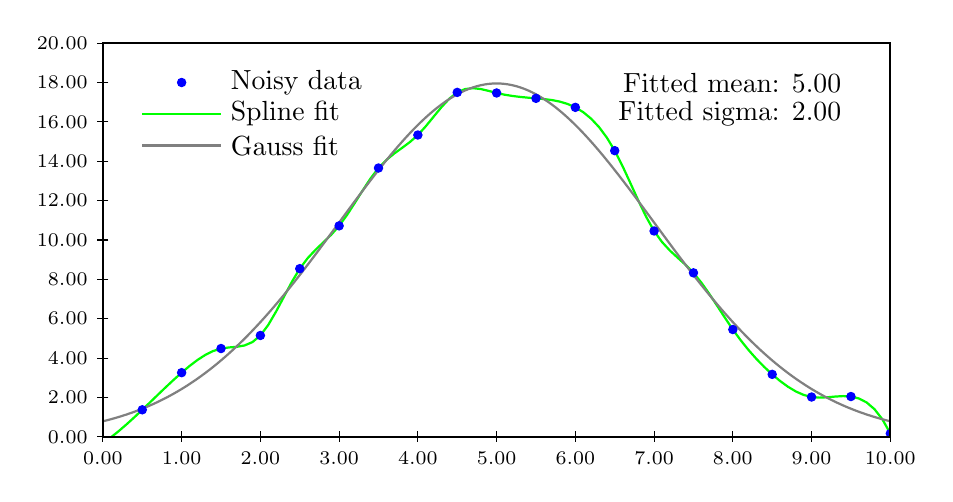
\begin{tikzpicture}
\begin{scope}[]
\pgfpathmoveto{ \pgfpointxy {0.0} {0.0}}
\pgfpathlineto{ \pgfpointxy {10.0} {0.0}}
\pgfpathlineto{ \pgfpointxy {10.0} {5.0}}
\pgfpathlineto{ \pgfpointxy {0.0} {5.0}}
\pgfpathclose
\pgfusepath{  clip, }
\begin{scope}[shift={(0.0,0.0)}]
\pgfsetxvec{\pgfpoint{1.0cm}{0cm}}
\pgfsetyvec{\pgfpoint{0cm}{0.25cm}}
\begin{scope}[shift={(0.0,0.0)}]
\begin{scope}[green,thick]
\pgfpathmoveto{ \pgfpointxy {0.0} {-0.3220822684578466}}
\pgfpathlineto{ \pgfpointxy {0.1} {-0.03179540914739956}}
\pgfpathlineto{ \pgfpointxy {0.2} {0.2885428151650948}}
\pgfpathlineto{ \pgfpointxy {0.3} {0.633328152486329}}
\pgfpathlineto{ \pgfpointxy {0.4} {0.9969563508229966}}
\pgfpathlineto{ \pgfpointxy {0.5} {1.3738231581817897}}
\pgfpathlineto{ \pgfpointxy {0.6} {1.7583243225694014}}
\pgfpathlineto{ \pgfpointxy {0.7} {2.144855591992525}}
\pgfpathlineto{ \pgfpointxy {0.8} {2.5278127144578533}}
\pgfpathlineto{ \pgfpointxy {0.9} {2.9015914379720784}}
\pgfpathlineto{ \pgfpointxy {1.0} {3.2605875105418933}}
\pgfpathlineto{ \pgfpointxy {1.1} {3.59798429165626}}
\pgfpathlineto{ \pgfpointxy {1.2} {3.9021155867332062}}
\pgfpathlineto{ \pgfpointxy {1.3} {4.160102812673034}}
\pgfpathlineto{ \pgfpointxy {1.4} {4.359067386376038}}
\pgfpathlineto{ \pgfpointxy {1.5} {4.486130724742518}}
\pgfpathlineto{ \pgfpointxy {1.6} {4.540874002276166}}
\pgfpathlineto{ \pgfpointxy {1.7} {4.572717423894254}}
\pgfpathlineto{ \pgfpointxy {1.8} {4.6435409521174424}}
\pgfpathlineto{ \pgfpointxy {1.9} {4.815224549466396}}
\pgfpathlineto{ \pgfpointxy {2.0} {5.149648178461778}}
\pgfpathlineto{ \pgfpointxy {2.1} {5.685601299272113}}
\pgfpathlineto{ \pgfpointxy {2.2} {6.3695113626573665}}
\pgfpathlineto{ \pgfpointxy {2.3} {7.124715317025358}}
\pgfpathlineto{ \pgfpointxy {2.4} {7.874550110783923}}
\pgfpathlineto{ \pgfpointxy {2.5} {8.54235269234088}}
\pgfpathlineto{ \pgfpointxy {2.6} {9.073464969531473}}
\pgfpathlineto{ \pgfpointxy {2.7} {9.50124868790061}}
\pgfpathlineto{ \pgfpointxy {2.8} {9.88107055242061}}
\pgfpathlineto{ \pgfpointxy {2.9} {10.268297268063803}}
\pgfpathlineto{ \pgfpointxy {3.0} {10.718295539802511}}
\pgfpathlineto{ \pgfpointxy {3.1} {11.268900377785958}}
\pgfpathlineto{ \pgfpointxy {3.2} {11.887820012870971}}
\pgfpathlineto{ \pgfpointxy {3.3} {12.52523098109127}}
\pgfpathlineto{ \pgfpointxy {3.4} {13.131309818480585}}
\pgfpathlineto{ \pgfpointxy {3.5} {13.656233061072639}}
\pgfpathlineto{ \pgfpointxy {3.6} {14.066283096326574}}
\pgfpathlineto{ \pgfpointxy {3.7} {14.392165717403207}}
\pgfpathlineto{ \pgfpointxy {3.8} {14.680692568888766}}
\pgfpathlineto{ \pgfpointxy {3.9} {14.978675295369484}}
\pgfpathlineto{ \pgfpointxy {4.0} {15.3329255414316}}
\pgfpathlineto{ \pgfpointxy {4.1} {15.773545607044694}}
\pgfpathlineto{ \pgfpointxy {4.2} {16.263800413711795}}
\pgfpathlineto{ \pgfpointxy {4.3} {16.75024553831928}}
\pgfpathlineto{ \pgfpointxy {4.4} {17.179436557753533}}
\pgfpathlineto{ \pgfpointxy {4.5} {17.497929048900925}}
\pgfpathlineto{ \pgfpointxy {4.6} {17.667544878429773}}
\pgfpathlineto{ \pgfpointxy {4.7} {17.711171072136075}}
\pgfpathlineto{ \pgfpointxy {4.8} {17.666960945597783}}
\pgfpathlineto{ \pgfpointxy {4.9} {17.57306781439283}}
\pgfpathlineto{ \pgfpointxy {5.0} {17.46764499409915}}
\pgfpathlineto{ \pgfpointxy {5.1} {17.38158457781227}}
\pgfpathlineto{ \pgfpointxy {5.2} {17.31673376869809}}
\pgfpathlineto{ \pgfpointxy {5.3} {17.267678547440084}}
\pgfpathlineto{ \pgfpointxy {5.4} {17.22900489472175}}
\pgfpathlineto{ \pgfpointxy {5.5} {17.195298791226566}}
\pgfpathlineto{ \pgfpointxy {5.6} {17.15975016321322}}
\pgfpathlineto{ \pgfpointxy {5.7} {17.109964719241223}}
\pgfpathlineto{ \pgfpointxy {5.8} {17.0321521134453}}
\pgfpathlineto{ \pgfpointxy {5.9} {16.912521999960166}}
\pgfpathlineto{ \pgfpointxy {6.0} {16.73728403292054}}
\pgfpathlineto{ \pgfpointxy {6.1} {16.492593096437812}}
\pgfpathlineto{ \pgfpointxy {6.2} {16.164384994530018}}
\pgfpathlineto{ \pgfpointxy {6.3} {15.738540761191885}}
\pgfpathlineto{ \pgfpointxy {6.4} {15.200941430418121}}
\pgfpathlineto{ \pgfpointxy {6.5} {14.537468036203448}}
\pgfpathlineto{ \pgfpointxy {6.6} {13.746955063475587}}
\pgfpathlineto{ \pgfpointxy {6.7} {12.880050800894296}}
\pgfpathlineto{ \pgfpointxy {6.8} {12.000356988052364}}
\pgfpathlineto{ \pgfpointxy {6.9} {11.171475364542555}}
\pgfpathlineto{ \pgfpointxy {7.0} {10.457007669957658}}
\pgfpathlineto{ \pgfpointxy {7.1} {9.900588706936261}}
\pgfpathlineto{ \pgfpointxy {7.2} {9.465985530300243}}
\pgfpathlineto{ \pgfpointxy {7.3} {9.096998257917303}}
\pgfpathlineto{ \pgfpointxy {7.4} {8.737427007655137}}
\pgfpathlineto{ \pgfpointxy {7.5} {8.331071897381452}}
\pgfpathlineto{ \pgfpointxy {7.6} {7.836306153830907}}
\pgfpathlineto{ \pgfpointxy {7.7} {7.269795439206012}}
\pgfpathlineto{ \pgfpointxy {7.8} {6.662778524576263}}
\pgfpathlineto{ \pgfpointxy {7.9} {6.046494181011129}}
\pgfpathlineto{ \pgfpointxy {8.0} {5.452181179580102}}
\pgfpathlineto{ \pgfpointxy {8.1} {4.905237179264141}}
\pgfpathlineto{ \pgfpointxy {8.2} {4.4076953906901215}}
\pgfpathlineto{ \pgfpointxy {8.3} {3.9557479123963915}}
\pgfpathlineto{ \pgfpointxy {8.4} {3.545586842921326}}
\pgfpathlineto{ \pgfpointxy {8.5} {3.173404280803272}}
\pgfpathlineto{ \pgfpointxy {8.6} {2.837587185462304}}
\pgfpathlineto{ \pgfpointxy {8.7} {2.545301959845368}}
\pgfpathlineto{ \pgfpointxy {8.8} {2.305909867781125}}
\pgfpathlineto{ \pgfpointxy {8.9} {2.128772173098246}}
\pgfpathlineto{ \pgfpointxy {9.0} {2.0232501396253917}}
\pgfpathlineto{ \pgfpointxy {9.1} {1.9919084111773382}}
\pgfpathlineto{ \pgfpointxy {9.2} {2.010125151513315}}
\pgfpathlineto{ \pgfpointxy {9.3} {2.046481904378665}}
\pgfpathlineto{ \pgfpointxy {9.4} {2.0695602135187294}}
\pgfpathlineto{ \pgfpointxy {9.5} {2.047941622678851}}
\pgfpathlineto{ \pgfpointxy {9.6} {1.9502076756043718}}
\pgfpathlineto{ \pgfpointxy {9.7} {1.744939916040635}}
\pgfpathlineto{ \pgfpointxy {9.8} {1.400719887732975}}
\pgfpathlineto{ \pgfpointxy {9.9} {0.8861291344267457}}
\pgfpathlineto{ \pgfpointxy {10.0} {0.16974919986728543}}
\pgfusepath{ stroke, }
\end{scope}
\begin{scope}[thick,gray]
\pgfpathmoveto{ \pgfpointxy {0.0} {0.7887735222102034}}
\pgfpathlineto{ \pgfpointxy {0.05} {0.8393826956517481}}
\pgfpathlineto{ \pgfpointxy {0.1} {0.892680947630374}}
\pgfpathlineto{ \pgfpointxy {0.15} {0.9487703099544526}}
\pgfpathlineto{ \pgfpointxy {0.2} {1.0077538632674794}}
\pgfpathlineto{ \pgfpointxy {0.25} {1.0697355373456514}}
\pgfpathlineto{ \pgfpointxy {0.3} {1.134819896183258}}
\pgfpathlineto{ \pgfpointxy {0.35} {1.203111907750662}}
\pgfpathlineto{ \pgfpointxy {0.4} {1.2747166983715252}}
\pgfpathlineto{ \pgfpointxy {0.45} {1.3497392917319906}}
\pgfpathlineto{ \pgfpointxy {0.5} {1.4282843326044656}}
\pgfpathlineto{ \pgfpointxy {0.55} {1.5104557954424003}}
\pgfpathlineto{ \pgfpointxy {0.6} {1.5963566780798044}}
\pgfpathlineto{ \pgfpointxy {0.65} {1.6860886808498898}}
\pgfpathlineto{ \pgfpointxy {0.7} {1.779751871521008}}
\pgfpathlineto{ \pgfpointxy {0.75} {1.8774443365345639}}
\pgfpathlineto{ \pgfpointxy {0.8} {1.9792618191185283}}
\pgfpathlineto{ \pgfpointxy {0.85} {2.0852973449411976}}
\pgfpathlineto{ \pgfpointxy {0.9} {2.1956408360624864}}
\pgfpathlineto{ \pgfpointxy {0.95} {2.310378714033865}}
\pgfpathlineto{ \pgfpointxy {1.0} {2.42959349309268}}
\pgfpathlineto{ \pgfpointxy {1.05} {2.5533633644912777}}
\pgfpathlineto{ \pgfpointxy {1.1} {2.6817617730958987}}
\pgfpathlineto{ \pgfpointxy {1.15} {2.8148569874838527}}
\pgfpathlineto{ \pgfpointxy {1.2} {2.95271166485958}}
\pgfpathlineto{ \pgfpointxy {1.25} {3.0953824122002476}}
\pgfpathlineto{ \pgfpointxy {1.3} {3.2429193451289016}}
\pgfpathlineto{ \pgfpointxy {1.35} {3.3953656460971313}}
\pgfpathlineto{ \pgfpointxy {1.4} {3.5527571235392896}}
\pgfpathlineto{ \pgfpointxy {1.45} {3.7151217737356554}}
\pgfpathlineto{ \pgfpointxy {1.5} {3.882479347192031}}
\pgfpathlineto{ \pgfpointxy {1.55} {4.0548409214074095}}
\pgfpathlineto{ \pgfpointxy {1.6} {4.232208481958889}}
\pgfpathlineto{ \pgfpointxy {1.65} {4.414574513883361}}
\pgfpathlineto{ \pgfpointxy {1.7} {4.601921605377953}}
\pgfpathlineto{ \pgfpointxy {1.75} {4.794222065875254}}
\pgfpathlineto{ \pgfpointxy {1.8} {4.991437560574411}}
\pgfpathlineto{ \pgfpointxy {1.85} {5.193518763524646}}
\pgfpathlineto{ \pgfpointxy {1.9} {5.400405031363236}}
\pgfpathlineto{ \pgfpointxy {1.95} {5.612024099804946}}
\pgfpathlineto{ \pgfpointxy {2.0} {5.828291804963986}}
\pgfpathlineto{ \pgfpointxy {2.05} {6.0491118315624055}}
\pgfpathlineto{ \pgfpointxy {2.1} {6.27437549004005}}
\pgfpathlineto{ \pgfpointxy {2.15} {6.503961524530807}}
\pgfpathlineto{ \pgfpointxy {2.2} {6.7377359536073405}}
\pgfpathlineto{ \pgfpointxy {2.25} {6.975551945622008}}
\pgfpathlineto{ \pgfpointxy {2.3} {7.217249730385189}}
\pgfpathlineto{ \pgfpointxy {2.35} {7.462656548823516}}
\pgfpathlineto{ \pgfpointxy {2.4} {7.71158664215013}}
\pgfpathlineto{ \pgfpointxy {2.45} {7.963841281956886}}
\pgfpathlineto{ \pgfpointxy {2.5} {8.219208842504782}}
\pgfpathlineto{ \pgfpointxy {2.55} {8.47746491634448}}
\pgfpathlineto{ \pgfpointxy {2.6} {8.73837247424338}}
\pgfpathlineto{ \pgfpointxy {2.65} {9.001682070230748}}
\pgfpathlineto{ \pgfpointxy {2.7} {9.267132092397667}}
\pgfpathlineto{ \pgfpointxy {2.75} {9.534449059905283}}
\pgfpathlineto{ \pgfpointxy {2.8} {9.803347966463585}}
\pgfpathlineto{ \pgfpointxy {2.85} {10.073532670344598}}
\pgfpathlineto{ \pgfpointxy {2.9} {10.344696330789311}}
\pgfpathlineto{ \pgfpointxy {2.95} {10.6165218904581}}
\pgfpathlineto{ \pgfpointxy {3.0} {10.888682603360296}}
\pgfpathlineto{ \pgfpointxy {3.05} {11.160842607482026}}
\pgfpathlineto{ \pgfpointxy {3.1} {11.432657541112373}}
\pgfpathlineto{ \pgfpointxy {3.15} {11.703775201648687}}
\pgfpathlineto{ \pgfpointxy {3.2} {11.973836245442861}}
\pgfpathlineto{ \pgfpointxy {3.25} {12.242474927033365}}
\pgfpathlineto{ \pgfpointxy {3.3} {12.509319875893764}}
\pgfpathlineto{ \pgfpointxy {3.35} {12.773994908618867}}
\pgfpathlineto{ \pgfpointxy {3.4} {13.036119874265678}}
\pgfpathlineto{ \pgfpointxy {3.45} {13.295311530369304}}
\pgfpathlineto{ \pgfpointxy {3.5} {13.551184446965188}}
\pgfpathlineto{ \pgfpointxy {3.55} {13.803351935769804}}
\pgfpathlineto{ \pgfpointxy {3.6} {14.051427001503281}}
\pgfpathlineto{ \pgfpointxy {3.65} {14.295023312180714}}
\pgfpathlineto{ \pgfpointxy {3.7} {14.533756185055205}}
\pgfpathlineto{ \pgfpointxy {3.75} {14.767243584765959}}
\pgfpathlineto{ \pgfpointxy {3.8} {14.995107130130082}}
\pgfpathlineto{ \pgfpointxy {3.85} {15.216973105918132}}
\pgfpathlineto{ \pgfpointxy {3.9} {15.432473475871411}}
\pgfpathlineto{ \pgfpointxy {3.95} {15.64124689315482}}
\pgfpathlineto{ \pgfpointxy {4.0} {15.84293970439265}}
\pgfpathlineto{ \pgfpointxy {4.05} {16.037206943407437}}
\pgfpathlineto{ \pgfpointxy {4.1} {16.223713310773366}}
\pgfpathlineto{ \pgfpointxy {4.15} {16.40213413530702}}
\pgfpathlineto{ \pgfpointxy {4.2} {16.572156313648794}}
\pgfpathlineto{ \pgfpointxy {4.25} {16.73347922413886}}
\pgfpathlineto{ \pgfpointxy {4.3} {16.885815611261478}}
\pgfpathlineto{ \pgfpointxy {4.35} {17.028892437021163}}
\pgfpathlineto{ \pgfpointxy {4.4} {17.162451695722886}}
\pgfpathlineto{ \pgfpointxy {4.45} {17.28625118875603}}
\pgfpathlineto{ \pgfpointxy {4.5} {17.40006525612754}}
\pgfpathlineto{ \pgfpointxy {4.55} {17.503685461653063}}
\pgfpathlineto{ \pgfpointxy {4.6} {17.596921228894864}}
\pgfpathlineto{ \pgfpointxy {4.65} {17.679600425131426}}
\pgfpathlineto{ \pgfpointxy {4.7} {17.751569890854366}}
\pgfpathlineto{ \pgfpointxy {4.75} {17.8126959125131}}
\pgfpathlineto{ \pgfpointxy {4.8} {17.862864636464906}}
\pgfpathlineto{ \pgfpointxy {4.85} {17.90198242233675}}
\pgfpathlineto{ \pgfpointxy {4.9} {17.929976134263764}}
\pgfpathlineto{ \pgfpointxy {4.95} {17.946793368736568}}
\pgfpathlineto{ \pgfpointxy {5.0} {17.952402618063857}}
\pgfpathlineto{ \pgfpointxy {5.05} {17.946793368736568}}
\pgfpathlineto{ \pgfpointxy {5.1} {17.929976134263764}}
\pgfpathlineto{ \pgfpointxy {5.15} {17.90198242233675}}
\pgfpathlineto{ \pgfpointxy {5.2} {17.862864636464906}}
\pgfpathlineto{ \pgfpointxy {5.25} {17.8126959125131}}
\pgfpathlineto{ \pgfpointxy {5.3} {17.751569890854366}}
\pgfpathlineto{ \pgfpointxy {5.35} {17.679600425131426}}
\pgfpathlineto{ \pgfpointxy {5.4} {17.596921228894864}}
\pgfpathlineto{ \pgfpointxy {5.45} {17.503685461653063}}
\pgfpathlineto{ \pgfpointxy {5.5} {17.40006525612754}}
\pgfpathlineto{ \pgfpointxy {5.55} {17.28625118875603}}
\pgfpathlineto{ \pgfpointxy {5.6} {17.162451695722886}}
\pgfpathlineto{ \pgfpointxy {5.65} {17.028892437021163}}
\pgfpathlineto{ \pgfpointxy {5.7} {16.885815611261478}}
\pgfpathlineto{ \pgfpointxy {5.75} {16.73347922413886}}
\pgfpathlineto{ \pgfpointxy {5.8} {16.572156313648794}}
\pgfpathlineto{ \pgfpointxy {5.85} {16.40213413530702}}
\pgfpathlineto{ \pgfpointxy {5.9} {16.223713310773366}}
\pgfpathlineto{ \pgfpointxy {5.95} {16.037206943407437}}
\pgfpathlineto{ \pgfpointxy {6.0} {15.84293970439265}}
\pgfpathlineto{ \pgfpointxy {6.05} {15.64124689315482}}
\pgfpathlineto{ \pgfpointxy {6.1} {15.432473475871413}}
\pgfpathlineto{ \pgfpointxy {6.15} {15.21697310591813}}
\pgfpathlineto{ \pgfpointxy {6.2} {14.995107130130082}}
\pgfpathlineto{ \pgfpointxy {6.25} {14.767243584765959}}
\pgfpathlineto{ \pgfpointxy {6.3} {14.533756185055205}}
\pgfpathlineto{ \pgfpointxy {6.35} {14.295023312180716}}
\pgfpathlineto{ \pgfpointxy {6.4} {14.05142700150328}}
\pgfpathlineto{ \pgfpointxy {6.45} {13.803351935769804}}
\pgfpathlineto{ \pgfpointxy {6.5} {13.551184446965188}}
\pgfpathlineto{ \pgfpointxy {6.55} {13.295311530369304}}
\pgfpathlineto{ \pgfpointxy {6.6} {13.03611987426568}}
\pgfpathlineto{ \pgfpointxy {6.65} {12.773994908618866}}
\pgfpathlineto{ \pgfpointxy {6.7} {12.509319875893764}}
\pgfpathlineto{ \pgfpointxy {6.75} {12.242474927033365}}
\pgfpathlineto{ \pgfpointxy {6.8} {11.973836245442861}}
\pgfpathlineto{ \pgfpointxy {6.85} {11.70377520164869}}
\pgfpathlineto{ \pgfpointxy {6.9} {11.43265754111237}}
\pgfpathlineto{ \pgfpointxy {6.95} {11.160842607482026}}
\pgfpathlineto{ \pgfpointxy {7.0} {10.888682603360296}}
\pgfpathlineto{ \pgfpointxy {7.05} {10.6165218904581}}
\pgfpathlineto{ \pgfpointxy {7.1} {10.344696330789315}}
\pgfpathlineto{ \pgfpointxy {7.15} {10.073532670344594}}
\pgfpathlineto{ \pgfpointxy {7.2} {9.803347966463585}}
\pgfpathlineto{ \pgfpointxy {7.25} {9.534449059905283}}
\pgfpathlineto{ \pgfpointxy {7.3} {9.267132092397667}}
\pgfpathlineto{ \pgfpointxy {7.35} {9.00168207023075}}
\pgfpathlineto{ \pgfpointxy {7.4} {8.738372474243379}}
\pgfpathlineto{ \pgfpointxy {7.45} {8.47746491634448}}
\pgfpathlineto{ \pgfpointxy {7.5} {8.219208842504782}}
\pgfpathlineto{ \pgfpointxy {7.55} {7.963841281956886}}
\pgfpathlineto{ \pgfpointxy {7.6} {7.711586642150132}}
\pgfpathlineto{ \pgfpointxy {7.65} {7.462656548823513}}
\pgfpathlineto{ \pgfpointxy {7.7} {7.217249730385189}}
\pgfpathlineto{ \pgfpointxy {7.75} {6.975551945622008}}
\pgfpathlineto{ \pgfpointxy {7.8} {6.7377359536073405}}
\pgfpathlineto{ \pgfpointxy {7.85} {6.503961524530809}}
\pgfpathlineto{ \pgfpointxy {7.9} {6.274375490040049}}
\pgfpathlineto{ \pgfpointxy {7.95} {6.0491118315624055}}
\pgfpathlineto{ \pgfpointxy {8.0} {5.828291804963986}}
\pgfpathlineto{ \pgfpointxy {8.05} {5.612024099804942}}
\pgfpathlineto{ \pgfpointxy {8.1} {5.4004050313632375}}
\pgfpathlineto{ \pgfpointxy {8.15} {5.193518763524644}}
\pgfpathlineto{ \pgfpointxy {8.2} {4.991437560574414}}
\pgfpathlineto{ \pgfpointxy {8.25} {4.794222065875254}}
\pgfpathlineto{ \pgfpointxy {8.3} {4.60192160537795}}
\pgfpathlineto{ \pgfpointxy {8.35} {4.4145745138833625}}
\pgfpathlineto{ \pgfpointxy {8.4} {4.232208481958887}}
\pgfpathlineto{ \pgfpointxy {8.45} {4.054840921407412}}
\pgfpathlineto{ \pgfpointxy {8.5} {3.882479347192031}}
\pgfpathlineto{ \pgfpointxy {8.55} {3.7151217737356528}}
\pgfpathlineto{ \pgfpointxy {8.6} {3.55275712353929}}
\pgfpathlineto{ \pgfpointxy {8.65} {3.3953656460971304}}
\pgfpathlineto{ \pgfpointxy {8.7} {3.2429193451289042}}
\pgfpathlineto{ \pgfpointxy {8.75} {3.0953824122002476}}
\pgfpathlineto{ \pgfpointxy {8.8} {2.9527116648595775}}
\pgfpathlineto{ \pgfpointxy {8.85} {2.8148569874838545}}
\pgfpathlineto{ \pgfpointxy {8.9} {2.681761773095898}}
\pgfpathlineto{ \pgfpointxy {8.95} {2.55336336449128}}
\pgfpathlineto{ \pgfpointxy {9.0} {2.42959349309268}}
\pgfpathlineto{ \pgfpointxy {9.05} {2.310378714033863}}
\pgfpathlineto{ \pgfpointxy {9.1} {2.1956408360624864}}
\pgfpathlineto{ \pgfpointxy {9.15} {2.0852973449411976}}
\pgfpathlineto{ \pgfpointxy {9.2} {1.97926181911853}}
\pgfpathlineto{ \pgfpointxy {9.25} {1.8774443365345639}}
\pgfpathlineto{ \pgfpointxy {9.3} {1.7797518715210063}}
\pgfpathlineto{ \pgfpointxy {9.35} {1.6860886808498898}}
\pgfpathlineto{ \pgfpointxy {9.4} {1.5963566780798044}}
\pgfpathlineto{ \pgfpointxy {9.45} {1.5104557954424018}}
\pgfpathlineto{ \pgfpointxy {9.5} {1.4282843326044656}}
\pgfpathlineto{ \pgfpointxy {9.55} {1.3497392917319893}}
\pgfpathlineto{ \pgfpointxy {9.6} {1.2747166983715252}}
\pgfpathlineto{ \pgfpointxy {9.65} {1.203111907750662}}
\pgfpathlineto{ \pgfpointxy {9.7} {1.1348198961832596}}
\pgfpathlineto{ \pgfpointxy {9.75} {1.0697355373456514}}
\pgfpathlineto{ \pgfpointxy {9.8} {1.0077538632674785}}
\pgfpathlineto{ \pgfpointxy {9.85} {0.9487703099544526}}
\pgfpathlineto{ \pgfpointxy {9.9} {0.892680947630374}}
\pgfpathlineto{ \pgfpointxy {9.95} {0.8393826956517488}}
\pgfpathlineto{ \pgfpointxy {10.0} {0.7887735222102034}}
\pgfusepath{ stroke, }
\end{scope}
\node at (0.0,-0.3220822684578466) [circle,inner sep=0.0pt,minimum width =3.0pt,minimum height=3.0pt,draw=blue,fill=blue] {}; 
\node at (0.5,1.3738231581817897) [circle,inner sep=0.0pt,minimum width =3.0pt,minimum height=3.0pt,draw=blue,fill=blue] {}; 
\node at (1.0,3.2605875105418933) [circle,inner sep=0.0pt,minimum width =3.0pt,minimum height=3.0pt,draw=blue,fill=blue] {}; 
\node at (1.5,4.486130724742518) [circle,inner sep=0.0pt,minimum width =3.0pt,minimum height=3.0pt,draw=blue,fill=blue] {}; 
\node at (2.0,5.149648178461778) [circle,inner sep=0.0pt,minimum width =3.0pt,minimum height=3.0pt,draw=blue,fill=blue] {}; 
\node at (2.5,8.54235269234088) [circle,inner sep=0.0pt,minimum width =3.0pt,minimum height=3.0pt,draw=blue,fill=blue] {}; 
\node at (3.0,10.718295539802511) [circle,inner sep=0.0pt,minimum width =3.0pt,minimum height=3.0pt,draw=blue,fill=blue] {}; 
\node at (3.5,13.656233061072639) [circle,inner sep=0.0pt,minimum width =3.0pt,minimum height=3.0pt,draw=blue,fill=blue] {}; 
\node at (4.0,15.3329255414316) [circle,inner sep=0.0pt,minimum width =3.0pt,minimum height=3.0pt,draw=blue,fill=blue] {}; 
\node at (4.5,17.497929048900925) [circle,inner sep=0.0pt,minimum width =3.0pt,minimum height=3.0pt,draw=blue,fill=blue] {}; 
\node at (5.0,17.467644994099146) [circle,inner sep=0.0pt,minimum width =3.0pt,minimum height=3.0pt,draw=blue,fill=blue] {}; 
\node at (5.5,17.195298791226566) [circle,inner sep=0.0pt,minimum width =3.0pt,minimum height=3.0pt,draw=blue,fill=blue] {}; 
\node at (6.0,16.73728403292054) [circle,inner sep=0.0pt,minimum width =3.0pt,minimum height=3.0pt,draw=blue,fill=blue] {}; 
\node at (6.5,14.537468036203448) [circle,inner sep=0.0pt,minimum width =3.0pt,minimum height=3.0pt,draw=blue,fill=blue] {}; 
\node at (7.0,10.457007669957658) [circle,inner sep=0.0pt,minimum width =3.0pt,minimum height=3.0pt,draw=blue,fill=blue] {}; 
\node at (7.5,8.331071897381452) [circle,inner sep=0.0pt,minimum width =3.0pt,minimum height=3.0pt,draw=blue,fill=blue] {}; 
\node at (8.0,5.452181179580102) [circle,inner sep=0.0pt,minimum width =3.0pt,minimum height=3.0pt,draw=blue,fill=blue] {}; 
\node at (8.5,3.173404280803272) [circle,inner sep=0.0pt,minimum width =3.0pt,minimum height=3.0pt,draw=blue,fill=blue] {}; 
\node at (9.0,2.0232501396253917) [circle,inner sep=0.0pt,minimum width =3.0pt,minimum height=3.0pt,draw=blue,fill=blue] {}; 
\node at (9.5,2.047941622678851) [circle,inner sep=0.0pt,minimum width =3.0pt,minimum height=3.0pt,draw=blue,fill=blue] {}; 
\node at (10.0,0.16974919986728554) [circle,inner sep=0.0pt,minimum width =3.0pt,minimum height=3.0pt,draw=blue,fill=blue] {}; 
\end{scope}
\pgfsetxvec{\pgfpoint{1cm}{0cm}}
\pgfsetyvec{\pgfpoint{0cm}{1cm}}
\end{scope}
\end{scope}
\begin{scope}[shift={(0.0,0.0)}]
\pgfsetxvec{\pgfpoint{1.0cm}{0cm}}
\pgfsetyvec{\pgfpoint{0cm}{0.25cm}}
\begin{scope}[shift={(0.0,0.0)}]
\begin{scope}[yshift=0cm]
\draw[black] [shift={(0.0,0.0)}] (0,2pt) -- (0,-2pt) node[below]{ \scriptsize{\num[round-mode=places,round-precision=2]{0}}};
\draw[black] [shift={(1.0,0.0)}] (0,2pt) -- (0,-2pt) node[below]{ \scriptsize{\num[round-mode=places,round-precision=2]{1}}};
\draw[black] [shift={(2.0,0.0)}] (0,2pt) -- (0,-2pt) node[below]{ \scriptsize{\num[round-mode=places,round-precision=2]{2}}};
\draw[black] [shift={(3.0,0.0)}] (0,2pt) -- (0,-2pt) node[below]{ \scriptsize{\num[round-mode=places,round-precision=2]{3}}};
\draw[black] [shift={(4.0,0.0)}] (0,2pt) -- (0,-2pt) node[below]{ \scriptsize{\num[round-mode=places,round-precision=2]{4}}};
\draw[black] [shift={(5.0,0.0)}] (0,2pt) -- (0,-2pt) node[below]{ \scriptsize{\num[round-mode=places,round-precision=2]{5}}};
\draw[black] [shift={(6.0,0.0)}] (0,2pt) -- (0,-2pt) node[below]{ \scriptsize{\num[round-mode=places,round-precision=2]{6}}};
\draw[black] [shift={(7.0,0.0)}] (0,2pt) -- (0,-2pt) node[below]{ \scriptsize{\num[round-mode=places,round-precision=2]{7}}};
\draw[black] [shift={(8.0,0.0)}] (0,2pt) -- (0,-2pt) node[below]{ \scriptsize{\num[round-mode=places,round-precision=2]{8}}};
\draw[black] [shift={(9.0,0.0)}] (0,2pt) -- (0,-2pt) node[below]{ \scriptsize{\num[round-mode=places,round-precision=2]{9}}};
\draw[black] [shift={(10.0,0.0)}] (0,2pt) -- (0,-2pt) node[below]{ \scriptsize{\num[round-mode=places,round-precision=2]{10}}};
\end{scope}
\begin{scope}[xshift=0cm]
\draw[black] [shift={(0.0,0.0)}] (2pt,0) -- (-2pt,0) node[left]{ \scriptsize{\num[round-mode=places,round-precision=2]{0}}};
\draw[black] [shift={(0.0,2.0)}] (2pt,0) -- (-2pt,0) node[left]{ \scriptsize{\num[round-mode=places,round-precision=2]{2}}};
\draw[black] [shift={(0.0,4.0)}] (2pt,0) -- (-2pt,0) node[left]{ \scriptsize{\num[round-mode=places,round-precision=2]{4}}};
\draw[black] [shift={(0.0,6.0)}] (2pt,0) -- (-2pt,0) node[left]{ \scriptsize{\num[round-mode=places,round-precision=2]{6}}};
\draw[black] [shift={(0.0,8.0)}] (2pt,0) -- (-2pt,0) node[left]{ \scriptsize{\num[round-mode=places,round-precision=2]{8}}};
\draw[black] [shift={(0.0,10.0)}] (2pt,0) -- (-2pt,0) node[left]{ \scriptsize{\num[round-mode=places,round-precision=2]{10}}};
\draw[black] [shift={(0.0,12.0)}] (2pt,0) -- (-2pt,0) node[left]{ \scriptsize{\num[round-mode=places,round-precision=2]{12}}};
\draw[black] [shift={(0.0,14.0)}] (2pt,0) -- (-2pt,0) node[left]{ \scriptsize{\num[round-mode=places,round-precision=2]{14}}};
\draw[black] [shift={(0.0,16.0)}] (2pt,0) -- (-2pt,0) node[left]{ \scriptsize{\num[round-mode=places,round-precision=2]{16}}};
\draw[black] [shift={(0.0,18.0)}] (2pt,0) -- (-2pt,0) node[left]{ \scriptsize{\num[round-mode=places,round-precision=2]{18}}};
\draw[black] [shift={(0.0,20.0)}] (2pt,0) -- (-2pt,0) node[left]{ \scriptsize{\num[round-mode=places,round-precision=2]{20}}};
\end{scope}
\begin{scope}[thick,black,fill=white]
\pgfpathmoveto{ \pgfpointxy {0.0} {0.0}}
\pgfpathlineto{ \pgfpointxy {10.0} {0.0}}
\pgfpathlineto{ \pgfpointxy {10.0} {20.0}}
\pgfpathlineto{ \pgfpointxy {0.0} {20.0}}
\pgfpathclose
\pgfusepath{ stroke, }
\end{scope}
\end{scope}
\pgfsetxvec{\pgfpoint{1cm}{0cm}}
\pgfsetyvec{\pgfpoint{0cm}{1cm}}
\end{scope}
\node at (1.0,4.5) [circle,inner sep=0.0pt,minimum width =3.0pt,minimum height=3.0pt,draw=blue,fill=blue] {}; 
\node[right,] at (1.5,4.5) {Noisy data};
\draw[draw=green,thick] (0.5,4.1) -- (1.5,4.1);
\node[right,] at (1.5,4.1) {Spline fit};
\draw[thick,gray] (0.5,3.7) -- (1.5,3.7);
\node[right,] at (1.5,3.7) {Gauss fit};
\node[left] at (9.5,4.5) {Fitted mean:  5.00};
\node[left] at (9.5,4.1) {Fitted sigma:  2.00};
\end{tikzpicture}
\end{document}

  \caption{The Gaussian function fitted to a set of noisy measurements}
\end{figure}

\begin{figure}[H]
  \centering
  \documentclass{standalone}
\ifx\HCode\UnDef\else\def\pgfsysdriver{pgfsys-tex4ht.def}\fi
\usepackage{tikz}
\usepackage{color}
\usepackage{siunitx}
\usetikzlibrary{arrows,shapes}
\begin{document}
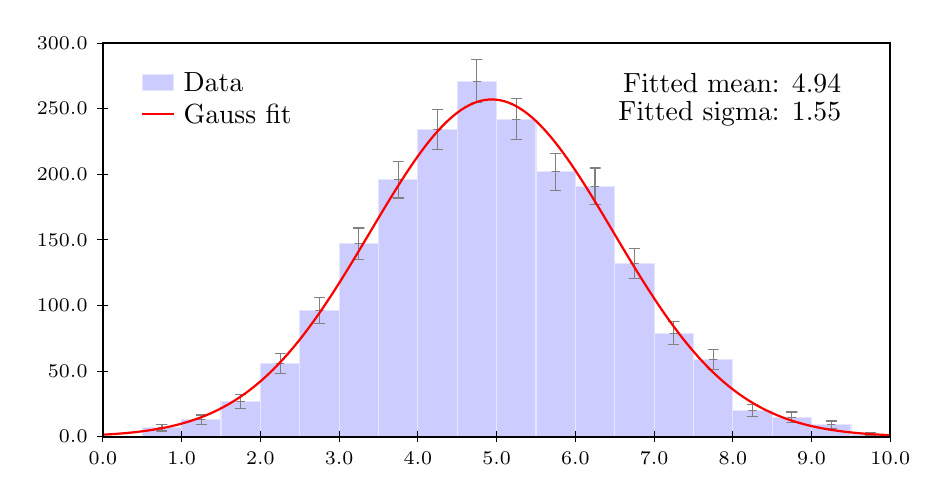
\begin{tikzpicture}
\node[left] at (9.5,4.5) {Fitted mean:  4.94};
\node[left] at (9.5,4.1) {Fitted sigma:  1.55};
\begin{scope}[]
\pgfpathmoveto{ \pgfpointxy {0.0} {0.0}}
\pgfpathlineto{ \pgfpointxy {10.0} {0.0}}
\pgfpathlineto{ \pgfpointxy {10.0} {5.0}}
\pgfpathlineto{ \pgfpointxy {0.0} {5.0}}
\pgfpathclose
\pgfusepath{  clip, }
\begin{scope}[shift={(0.0,0.0)}]
\pgfsetxvec{\pgfpoint{1.0cm}{0cm}}
\pgfsetyvec{\pgfpoint{0cm}{0.016666668cm}}
\begin{scope}[shift={(0.0,0.0)}]
\begin{scope}[draw=blue!10,fill=blue!20]
\pgfpathmoveto{ \pgfpointxy {10.0} {0.0}}
\pgfpathlineto{ \pgfpointxy {10.0} {2.0}}
\pgfpathlineto{ \pgfpointxy {9.5} {2.0}}
\pgfpathlineto{ \pgfpointxy {9.5} {9.0}}
\pgfpathlineto{ \pgfpointxy {9.0} {9.0}}
\pgfpathlineto{ \pgfpointxy {9.0} {15.0}}
\pgfpathlineto{ \pgfpointxy {8.5} {15.0}}
\pgfpathlineto{ \pgfpointxy {8.5} {20.0}}
\pgfpathlineto{ \pgfpointxy {8.0} {20.0}}
\pgfpathlineto{ \pgfpointxy {8.0} {59.0}}
\pgfpathlineto{ \pgfpointxy {7.5} {59.0}}
\pgfpathlineto{ \pgfpointxy {7.5} {79.0}}
\pgfpathlineto{ \pgfpointxy {7.0} {79.0}}
\pgfpathlineto{ \pgfpointxy {7.0} {132.0}}
\pgfpathlineto{ \pgfpointxy {6.5} {132.0}}
\pgfpathlineto{ \pgfpointxy {6.5} {191.0}}
\pgfpathlineto{ \pgfpointxy {6.0} {191.0}}
\pgfpathlineto{ \pgfpointxy {6.0} {202.0}}
\pgfpathlineto{ \pgfpointxy {5.5} {202.0}}
\pgfpathlineto{ \pgfpointxy {5.5} {242.0}}
\pgfpathlineto{ \pgfpointxy {5.0} {242.0}}
\pgfpathlineto{ \pgfpointxy {5.0} {271.0}}
\pgfpathlineto{ \pgfpointxy {4.5} {271.0}}
\pgfpathlineto{ \pgfpointxy {4.5} {234.0}}
\pgfpathlineto{ \pgfpointxy {4.0} {234.0}}
\pgfpathlineto{ \pgfpointxy {4.0} {196.0}}
\pgfpathlineto{ \pgfpointxy {3.5} {196.0}}
\pgfpathlineto{ \pgfpointxy {3.5} {147.0}}
\pgfpathlineto{ \pgfpointxy {3.0} {147.0}}
\pgfpathlineto{ \pgfpointxy {3.0} {96.0}}
\pgfpathlineto{ \pgfpointxy {2.5} {96.0}}
\pgfpathlineto{ \pgfpointxy {2.5} {56.0}}
\pgfpathlineto{ \pgfpointxy {2.0} {56.0}}
\pgfpathlineto{ \pgfpointxy {2.0} {27.0}}
\pgfpathlineto{ \pgfpointxy {1.5} {27.0}}
\pgfpathlineto{ \pgfpointxy {1.5} {13.0}}
\pgfpathlineto{ \pgfpointxy {1.0} {13.0}}
\pgfpathlineto{ \pgfpointxy {1.0} {7.0}}
\pgfpathlineto{ \pgfpointxy {0.5} {7.0}}
\pgfpathlineto{ \pgfpointxy {0.5} {0.0}}
\pgfpathlineto{ \pgfpointxy {0.0} {0.0}}
\pgfpathlineto{ \pgfpointxy {0.0} {0.0}}
\pgfusepath{ stroke, fill, }
\end{scope}
\begin{scope}[draw=blue!10,fill=blue!20]
\pgfpathmoveto{ \pgfpointxy {10.0} {0.0}}
\pgfpathlineto{ \pgfpointxy {10.0} {0.0}}
\pgfusepath{ stroke, }
\end{scope}
\begin{scope}[draw=blue!10,fill=blue!20]
\pgfpathmoveto{ \pgfpointxy {10.0} {2.0}}
\pgfpathlineto{ \pgfpointxy {10.0} {0.0}}
\pgfusepath{ stroke, }
\end{scope}
\begin{scope}[draw=blue!10,fill=blue!20]
\pgfpathmoveto{ \pgfpointxy {9.5} {2.0}}
\pgfpathlineto{ \pgfpointxy {9.5} {0.0}}
\pgfusepath{ stroke, }
\end{scope}
\begin{scope}[draw=blue!10,fill=blue!20]
\pgfpathmoveto{ \pgfpointxy {9.5} {9.0}}
\pgfpathlineto{ \pgfpointxy {9.5} {0.0}}
\pgfusepath{ stroke, }
\end{scope}
\begin{scope}[draw=blue!10,fill=blue!20]
\pgfpathmoveto{ \pgfpointxy {9.0} {9.0}}
\pgfpathlineto{ \pgfpointxy {9.0} {0.0}}
\pgfusepath{ stroke, }
\end{scope}
\begin{scope}[draw=blue!10,fill=blue!20]
\pgfpathmoveto{ \pgfpointxy {9.0} {15.0}}
\pgfpathlineto{ \pgfpointxy {9.0} {0.0}}
\pgfusepath{ stroke, }
\end{scope}
\begin{scope}[draw=blue!10,fill=blue!20]
\pgfpathmoveto{ \pgfpointxy {8.5} {15.0}}
\pgfpathlineto{ \pgfpointxy {8.5} {0.0}}
\pgfusepath{ stroke, }
\end{scope}
\begin{scope}[draw=blue!10,fill=blue!20]
\pgfpathmoveto{ \pgfpointxy {8.5} {20.0}}
\pgfpathlineto{ \pgfpointxy {8.5} {0.0}}
\pgfusepath{ stroke, }
\end{scope}
\begin{scope}[draw=blue!10,fill=blue!20]
\pgfpathmoveto{ \pgfpointxy {8.0} {20.0}}
\pgfpathlineto{ \pgfpointxy {8.0} {0.0}}
\pgfusepath{ stroke, }
\end{scope}
\begin{scope}[draw=blue!10,fill=blue!20]
\pgfpathmoveto{ \pgfpointxy {8.0} {59.0}}
\pgfpathlineto{ \pgfpointxy {8.0} {0.0}}
\pgfusepath{ stroke, }
\end{scope}
\begin{scope}[draw=blue!10,fill=blue!20]
\pgfpathmoveto{ \pgfpointxy {7.5} {59.0}}
\pgfpathlineto{ \pgfpointxy {7.5} {0.0}}
\pgfusepath{ stroke, }
\end{scope}
\begin{scope}[draw=blue!10,fill=blue!20]
\pgfpathmoveto{ \pgfpointxy {7.5} {79.0}}
\pgfpathlineto{ \pgfpointxy {7.5} {0.0}}
\pgfusepath{ stroke, }
\end{scope}
\begin{scope}[draw=blue!10,fill=blue!20]
\pgfpathmoveto{ \pgfpointxy {7.0} {79.0}}
\pgfpathlineto{ \pgfpointxy {7.0} {0.0}}
\pgfusepath{ stroke, }
\end{scope}
\begin{scope}[draw=blue!10,fill=blue!20]
\pgfpathmoveto{ \pgfpointxy {7.0} {132.0}}
\pgfpathlineto{ \pgfpointxy {7.0} {0.0}}
\pgfusepath{ stroke, }
\end{scope}
\begin{scope}[draw=blue!10,fill=blue!20]
\pgfpathmoveto{ \pgfpointxy {6.5} {132.0}}
\pgfpathlineto{ \pgfpointxy {6.5} {0.0}}
\pgfusepath{ stroke, }
\end{scope}
\begin{scope}[draw=blue!10,fill=blue!20]
\pgfpathmoveto{ \pgfpointxy {6.5} {191.0}}
\pgfpathlineto{ \pgfpointxy {6.5} {0.0}}
\pgfusepath{ stroke, }
\end{scope}
\begin{scope}[draw=blue!10,fill=blue!20]
\pgfpathmoveto{ \pgfpointxy {6.0} {191.0}}
\pgfpathlineto{ \pgfpointxy {6.0} {0.0}}
\pgfusepath{ stroke, }
\end{scope}
\begin{scope}[draw=blue!10,fill=blue!20]
\pgfpathmoveto{ \pgfpointxy {6.0} {202.0}}
\pgfpathlineto{ \pgfpointxy {6.0} {0.0}}
\pgfusepath{ stroke, }
\end{scope}
\begin{scope}[draw=blue!10,fill=blue!20]
\pgfpathmoveto{ \pgfpointxy {5.5} {202.0}}
\pgfpathlineto{ \pgfpointxy {5.5} {0.0}}
\pgfusepath{ stroke, }
\end{scope}
\begin{scope}[draw=blue!10,fill=blue!20]
\pgfpathmoveto{ \pgfpointxy {5.5} {242.0}}
\pgfpathlineto{ \pgfpointxy {5.5} {0.0}}
\pgfusepath{ stroke, }
\end{scope}
\begin{scope}[draw=blue!10,fill=blue!20]
\pgfpathmoveto{ \pgfpointxy {5.0} {242.0}}
\pgfpathlineto{ \pgfpointxy {5.0} {0.0}}
\pgfusepath{ stroke, }
\end{scope}
\begin{scope}[draw=blue!10,fill=blue!20]
\pgfpathmoveto{ \pgfpointxy {5.0} {271.0}}
\pgfpathlineto{ \pgfpointxy {5.0} {0.0}}
\pgfusepath{ stroke, }
\end{scope}
\begin{scope}[draw=blue!10,fill=blue!20]
\pgfpathmoveto{ \pgfpointxy {4.5} {271.0}}
\pgfpathlineto{ \pgfpointxy {4.5} {0.0}}
\pgfusepath{ stroke, }
\end{scope}
\begin{scope}[draw=blue!10,fill=blue!20]
\pgfpathmoveto{ \pgfpointxy {4.5} {234.0}}
\pgfpathlineto{ \pgfpointxy {4.5} {0.0}}
\pgfusepath{ stroke, }
\end{scope}
\begin{scope}[draw=blue!10,fill=blue!20]
\pgfpathmoveto{ \pgfpointxy {4.0} {234.0}}
\pgfpathlineto{ \pgfpointxy {4.0} {0.0}}
\pgfusepath{ stroke, }
\end{scope}
\begin{scope}[draw=blue!10,fill=blue!20]
\pgfpathmoveto{ \pgfpointxy {4.0} {196.0}}
\pgfpathlineto{ \pgfpointxy {4.0} {0.0}}
\pgfusepath{ stroke, }
\end{scope}
\begin{scope}[draw=blue!10,fill=blue!20]
\pgfpathmoveto{ \pgfpointxy {3.5} {196.0}}
\pgfpathlineto{ \pgfpointxy {3.5} {0.0}}
\pgfusepath{ stroke, }
\end{scope}
\begin{scope}[draw=blue!10,fill=blue!20]
\pgfpathmoveto{ \pgfpointxy {3.5} {147.0}}
\pgfpathlineto{ \pgfpointxy {3.5} {0.0}}
\pgfusepath{ stroke, }
\end{scope}
\begin{scope}[draw=blue!10,fill=blue!20]
\pgfpathmoveto{ \pgfpointxy {3.0} {147.0}}
\pgfpathlineto{ \pgfpointxy {3.0} {0.0}}
\pgfusepath{ stroke, }
\end{scope}
\begin{scope}[draw=blue!10,fill=blue!20]
\pgfpathmoveto{ \pgfpointxy {3.0} {96.0}}
\pgfpathlineto{ \pgfpointxy {3.0} {0.0}}
\pgfusepath{ stroke, }
\end{scope}
\begin{scope}[draw=blue!10,fill=blue!20]
\pgfpathmoveto{ \pgfpointxy {2.5} {96.0}}
\pgfpathlineto{ \pgfpointxy {2.5} {0.0}}
\pgfusepath{ stroke, }
\end{scope}
\begin{scope}[draw=blue!10,fill=blue!20]
\pgfpathmoveto{ \pgfpointxy {2.5} {56.0}}
\pgfpathlineto{ \pgfpointxy {2.5} {0.0}}
\pgfusepath{ stroke, }
\end{scope}
\begin{scope}[draw=blue!10,fill=blue!20]
\pgfpathmoveto{ \pgfpointxy {2.0} {56.0}}
\pgfpathlineto{ \pgfpointxy {2.0} {0.0}}
\pgfusepath{ stroke, }
\end{scope}
\begin{scope}[draw=blue!10,fill=blue!20]
\pgfpathmoveto{ \pgfpointxy {2.0} {27.0}}
\pgfpathlineto{ \pgfpointxy {2.0} {0.0}}
\pgfusepath{ stroke, }
\end{scope}
\begin{scope}[draw=blue!10,fill=blue!20]
\pgfpathmoveto{ \pgfpointxy {1.5} {27.0}}
\pgfpathlineto{ \pgfpointxy {1.5} {0.0}}
\pgfusepath{ stroke, }
\end{scope}
\begin{scope}[draw=blue!10,fill=blue!20]
\pgfpathmoveto{ \pgfpointxy {1.5} {13.0}}
\pgfpathlineto{ \pgfpointxy {1.5} {0.0}}
\pgfusepath{ stroke, }
\end{scope}
\begin{scope}[draw=blue!10,fill=blue!20]
\pgfpathmoveto{ \pgfpointxy {1.0} {13.0}}
\pgfpathlineto{ \pgfpointxy {1.0} {0.0}}
\pgfusepath{ stroke, }
\end{scope}
\begin{scope}[draw=blue!10,fill=blue!20]
\pgfpathmoveto{ \pgfpointxy {1.0} {7.0}}
\pgfpathlineto{ \pgfpointxy {1.0} {0.0}}
\pgfusepath{ stroke, }
\end{scope}
\begin{scope}[draw=blue!10,fill=blue!20]
\pgfpathmoveto{ \pgfpointxy {0.5} {7.0}}
\pgfpathlineto{ \pgfpointxy {0.5} {0.0}}
\pgfusepath{ stroke, }
\end{scope}
\begin{scope}[draw=blue!10,fill=blue!20]
\pgfpathmoveto{ \pgfpointxy {0.5} {0.0}}
\pgfpathlineto{ \pgfpointxy {0.5} {0.0}}
\pgfusepath{ stroke, }
\end{scope}
\begin{scope}[draw=blue!10,fill=blue!20]
\pgfpathmoveto{ \pgfpointxy {0.0} {0.0}}
\pgfpathlineto{ \pgfpointxy {0.0} {0.0}}
\pgfusepath{ stroke, }
\end{scope}
\begin{scope}[draw=blue!10,fill=blue!20]
\pgfpathmoveto{ \pgfpointxy {0.0} {0.0}}
\pgfpathlineto{ \pgfpointxy {0.0} {0.0}}
\pgfusepath{ stroke, }
\end{scope}
\begin{scope}[draw=gray,fill=gray]
\pgfpointadd{\pgfpointxy {0.25} {0.0}} {\pgfpoint{-2pt}{0}}\pgfpathmoveto{ NIL }
\pgfpointadd{\pgfpointxy {0.25} {0.0}} {\pgfpoint{2pt}{0}}\pgfpathlineto{ NIL }
\pgfpointadd{\pgfpointxy {0.25} {0.0}} {\pgfpoint{0pt}{0}}\pgfpathlineto{ NIL }
\pgfpointadd{\pgfpointxy {0.25} {0.0}} {\pgfpoint{0pt}{0}}\pgfpathlineto{ NIL }
\pgfpointadd{\pgfpointxy {0.25} {0.0}} {\pgfpoint{-2pt}{0}}\pgfpathlineto{ NIL }
\pgfpointadd{\pgfpointxy {0.25} {0.0}} {\pgfpoint{2pt}{0}}\pgfpathlineto{ NIL }
\pgfusepath{ stroke, }
\node at (0.25,0.0) [rectangle,inner sep=0.0pt,minimum width =3.0pt,minimum height=0.0pt,draw=gray,fill=gray] {}; 
\end{scope}
\begin{scope}[draw=gray,fill=gray]
\pgfpointadd{\pgfpointxy {0.75} {9.645751}} {\pgfpoint{-2pt}{0}}\pgfpathmoveto{ NIL }
\pgfpointadd{\pgfpointxy {0.75} {9.645751}} {\pgfpoint{2pt}{0}}\pgfpathlineto{ NIL }
\pgfpointadd{\pgfpointxy {0.75} {9.645751}} {\pgfpoint{0pt}{0}}\pgfpathlineto{ NIL }
\pgfpointadd{\pgfpointxy {0.75} {4.354249}} {\pgfpoint{0pt}{0}}\pgfpathlineto{ NIL }
\pgfpointadd{\pgfpointxy {0.75} {4.354249}} {\pgfpoint{-2pt}{0}}\pgfpathlineto{ NIL }
\pgfpointadd{\pgfpointxy {0.75} {4.354249}} {\pgfpoint{2pt}{0}}\pgfpathlineto{ NIL }
\pgfusepath{ stroke, }
\node at (0.75,7.0) [rectangle,inner sep=0.0pt,minimum width =3.0pt,minimum height=0.0pt,draw=gray,fill=gray] {}; 
\end{scope}
\begin{scope}[draw=gray,fill=gray]
\pgfpointadd{\pgfpointxy {1.25} {16.60555}} {\pgfpoint{-2pt}{0}}\pgfpathmoveto{ NIL }
\pgfpointadd{\pgfpointxy {1.25} {16.60555}} {\pgfpoint{2pt}{0}}\pgfpathlineto{ NIL }
\pgfpointadd{\pgfpointxy {1.25} {16.60555}} {\pgfpoint{0pt}{0}}\pgfpathlineto{ NIL }
\pgfpointadd{\pgfpointxy {1.25} {9.394449}} {\pgfpoint{0pt}{0}}\pgfpathlineto{ NIL }
\pgfpointadd{\pgfpointxy {1.25} {9.394449}} {\pgfpoint{-2pt}{0}}\pgfpathlineto{ NIL }
\pgfpointadd{\pgfpointxy {1.25} {9.394449}} {\pgfpoint{2pt}{0}}\pgfpathlineto{ NIL }
\pgfusepath{ stroke, }
\node at (1.25,13.0) [rectangle,inner sep=0.0pt,minimum width =3.0pt,minimum height=0.0pt,draw=gray,fill=gray] {}; 
\end{scope}
\begin{scope}[draw=gray,fill=gray]
\pgfpointadd{\pgfpointxy {1.75} {32.19615}} {\pgfpoint{-2pt}{0}}\pgfpathmoveto{ NIL }
\pgfpointadd{\pgfpointxy {1.75} {32.19615}} {\pgfpoint{2pt}{0}}\pgfpathlineto{ NIL }
\pgfpointadd{\pgfpointxy {1.75} {32.19615}} {\pgfpoint{0pt}{0}}\pgfpathlineto{ NIL }
\pgfpointadd{\pgfpointxy {1.75} {21.803848}} {\pgfpoint{0pt}{0}}\pgfpathlineto{ NIL }
\pgfpointadd{\pgfpointxy {1.75} {21.803848}} {\pgfpoint{-2pt}{0}}\pgfpathlineto{ NIL }
\pgfpointadd{\pgfpointxy {1.75} {21.803848}} {\pgfpoint{2pt}{0}}\pgfpathlineto{ NIL }
\pgfusepath{ stroke, }
\node at (1.75,27.0) [rectangle,inner sep=0.0pt,minimum width =3.0pt,minimum height=0.0pt,draw=gray,fill=gray] {}; 
\end{scope}
\begin{scope}[draw=gray,fill=gray]
\pgfpointadd{\pgfpointxy {2.25} {63.483315}} {\pgfpoint{-2pt}{0}}\pgfpathmoveto{ NIL }
\pgfpointadd{\pgfpointxy {2.25} {63.483315}} {\pgfpoint{2pt}{0}}\pgfpathlineto{ NIL }
\pgfpointadd{\pgfpointxy {2.25} {63.483315}} {\pgfpoint{0pt}{0}}\pgfpathlineto{ NIL }
\pgfpointadd{\pgfpointxy {2.25} {48.516685}} {\pgfpoint{0pt}{0}}\pgfpathlineto{ NIL }
\pgfpointadd{\pgfpointxy {2.25} {48.516685}} {\pgfpoint{-2pt}{0}}\pgfpathlineto{ NIL }
\pgfpointadd{\pgfpointxy {2.25} {48.516685}} {\pgfpoint{2pt}{0}}\pgfpathlineto{ NIL }
\pgfusepath{ stroke, }
\node at (2.25,56.0) [rectangle,inner sep=0.0pt,minimum width =3.0pt,minimum height=0.0pt,draw=gray,fill=gray] {}; 
\end{scope}
\begin{scope}[draw=gray,fill=gray]
\pgfpointadd{\pgfpointxy {2.75} {105.79796}} {\pgfpoint{-2pt}{0}}\pgfpathmoveto{ NIL }
\pgfpointadd{\pgfpointxy {2.75} {105.79796}} {\pgfpoint{2pt}{0}}\pgfpathlineto{ NIL }
\pgfpointadd{\pgfpointxy {2.75} {105.79796}} {\pgfpoint{0pt}{0}}\pgfpathlineto{ NIL }
\pgfpointadd{\pgfpointxy {2.75} {86.20204}} {\pgfpoint{0pt}{0}}\pgfpathlineto{ NIL }
\pgfpointadd{\pgfpointxy {2.75} {86.20204}} {\pgfpoint{-2pt}{0}}\pgfpathlineto{ NIL }
\pgfpointadd{\pgfpointxy {2.75} {86.20204}} {\pgfpoint{2pt}{0}}\pgfpathlineto{ NIL }
\pgfusepath{ stroke, }
\node at (2.75,96.0) [rectangle,inner sep=0.0pt,minimum width =3.0pt,minimum height=0.0pt,draw=gray,fill=gray] {}; 
\end{scope}
\begin{scope}[draw=gray,fill=gray]
\pgfpointadd{\pgfpointxy {3.25} {159.12436}} {\pgfpoint{-2pt}{0}}\pgfpathmoveto{ NIL }
\pgfpointadd{\pgfpointxy {3.25} {159.12436}} {\pgfpoint{2pt}{0}}\pgfpathlineto{ NIL }
\pgfpointadd{\pgfpointxy {3.25} {159.12436}} {\pgfpoint{0pt}{0}}\pgfpathlineto{ NIL }
\pgfpointadd{\pgfpointxy {3.25} {134.87564}} {\pgfpoint{0pt}{0}}\pgfpathlineto{ NIL }
\pgfpointadd{\pgfpointxy {3.25} {134.87564}} {\pgfpoint{-2pt}{0}}\pgfpathlineto{ NIL }
\pgfpointadd{\pgfpointxy {3.25} {134.87564}} {\pgfpoint{2pt}{0}}\pgfpathlineto{ NIL }
\pgfusepath{ stroke, }
\node at (3.25,147.0) [rectangle,inner sep=0.0pt,minimum width =3.0pt,minimum height=0.0pt,draw=gray,fill=gray] {}; 
\end{scope}
\begin{scope}[draw=gray,fill=gray]
\pgfpointadd{\pgfpointxy {3.75} {210.0}} {\pgfpoint{-2pt}{0}}\pgfpathmoveto{ NIL }
\pgfpointadd{\pgfpointxy {3.75} {210.0}} {\pgfpoint{2pt}{0}}\pgfpathlineto{ NIL }
\pgfpointadd{\pgfpointxy {3.75} {210.0}} {\pgfpoint{0pt}{0}}\pgfpathlineto{ NIL }
\pgfpointadd{\pgfpointxy {3.75} {182.0}} {\pgfpoint{0pt}{0}}\pgfpathlineto{ NIL }
\pgfpointadd{\pgfpointxy {3.75} {182.0}} {\pgfpoint{-2pt}{0}}\pgfpathlineto{ NIL }
\pgfpointadd{\pgfpointxy {3.75} {182.0}} {\pgfpoint{2pt}{0}}\pgfpathlineto{ NIL }
\pgfusepath{ stroke, }
\node at (3.75,196.0) [rectangle,inner sep=0.0pt,minimum width =3.0pt,minimum height=0.0pt,draw=gray,fill=gray] {}; 
\end{scope}
\begin{scope}[draw=gray,fill=gray]
\pgfpointadd{\pgfpointxy {4.25} {249.29706}} {\pgfpoint{-2pt}{0}}\pgfpathmoveto{ NIL }
\pgfpointadd{\pgfpointxy {4.25} {249.29706}} {\pgfpoint{2pt}{0}}\pgfpathlineto{ NIL }
\pgfpointadd{\pgfpointxy {4.25} {249.29706}} {\pgfpoint{0pt}{0}}\pgfpathlineto{ NIL }
\pgfpointadd{\pgfpointxy {4.25} {218.70294}} {\pgfpoint{0pt}{0}}\pgfpathlineto{ NIL }
\pgfpointadd{\pgfpointxy {4.25} {218.70294}} {\pgfpoint{-2pt}{0}}\pgfpathlineto{ NIL }
\pgfpointadd{\pgfpointxy {4.25} {218.70294}} {\pgfpoint{2pt}{0}}\pgfpathlineto{ NIL }
\pgfusepath{ stroke, }
\node at (4.25,234.0) [rectangle,inner sep=0.0pt,minimum width =3.0pt,minimum height=0.0pt,draw=gray,fill=gray] {}; 
\end{scope}
\begin{scope}[draw=gray,fill=gray]
\pgfpointadd{\pgfpointxy {4.75} {287.46207}} {\pgfpoint{-2pt}{0}}\pgfpathmoveto{ NIL }
\pgfpointadd{\pgfpointxy {4.75} {287.46207}} {\pgfpoint{2pt}{0}}\pgfpathlineto{ NIL }
\pgfpointadd{\pgfpointxy {4.75} {287.46207}} {\pgfpoint{0pt}{0}}\pgfpathlineto{ NIL }
\pgfpointadd{\pgfpointxy {4.75} {254.53792}} {\pgfpoint{0pt}{0}}\pgfpathlineto{ NIL }
\pgfpointadd{\pgfpointxy {4.75} {254.53792}} {\pgfpoint{-2pt}{0}}\pgfpathlineto{ NIL }
\pgfpointadd{\pgfpointxy {4.75} {254.53792}} {\pgfpoint{2pt}{0}}\pgfpathlineto{ NIL }
\pgfusepath{ stroke, }
\node at (4.75,271.0) [rectangle,inner sep=0.0pt,minimum width =3.0pt,minimum height=0.0pt,draw=gray,fill=gray] {}; 
\end{scope}
\begin{scope}[draw=gray,fill=gray]
\pgfpointadd{\pgfpointxy {5.25} {257.55634}} {\pgfpoint{-2pt}{0}}\pgfpathmoveto{ NIL }
\pgfpointadd{\pgfpointxy {5.25} {257.55634}} {\pgfpoint{2pt}{0}}\pgfpathlineto{ NIL }
\pgfpointadd{\pgfpointxy {5.25} {257.55634}} {\pgfpoint{0pt}{0}}\pgfpathlineto{ NIL }
\pgfpointadd{\pgfpointxy {5.25} {226.44365}} {\pgfpoint{0pt}{0}}\pgfpathlineto{ NIL }
\pgfpointadd{\pgfpointxy {5.25} {226.44365}} {\pgfpoint{-2pt}{0}}\pgfpathlineto{ NIL }
\pgfpointadd{\pgfpointxy {5.25} {226.44365}} {\pgfpoint{2pt}{0}}\pgfpathlineto{ NIL }
\pgfusepath{ stroke, }
\node at (5.25,242.0) [rectangle,inner sep=0.0pt,minimum width =3.0pt,minimum height=0.0pt,draw=gray,fill=gray] {}; 
\end{scope}
\begin{scope}[draw=gray,fill=gray]
\pgfpointadd{\pgfpointxy {5.75} {216.21268}} {\pgfpoint{-2pt}{0}}\pgfpathmoveto{ NIL }
\pgfpointadd{\pgfpointxy {5.75} {216.21268}} {\pgfpoint{2pt}{0}}\pgfpathlineto{ NIL }
\pgfpointadd{\pgfpointxy {5.75} {216.21268}} {\pgfpoint{0pt}{0}}\pgfpathlineto{ NIL }
\pgfpointadd{\pgfpointxy {5.75} {187.78732}} {\pgfpoint{0pt}{0}}\pgfpathlineto{ NIL }
\pgfpointadd{\pgfpointxy {5.75} {187.78732}} {\pgfpoint{-2pt}{0}}\pgfpathlineto{ NIL }
\pgfpointadd{\pgfpointxy {5.75} {187.78732}} {\pgfpoint{2pt}{0}}\pgfpathlineto{ NIL }
\pgfusepath{ stroke, }
\node at (5.75,202.0) [rectangle,inner sep=0.0pt,minimum width =3.0pt,minimum height=0.0pt,draw=gray,fill=gray] {}; 
\end{scope}
\begin{scope}[draw=gray,fill=gray]
\pgfpointadd{\pgfpointxy {6.25} {204.82028}} {\pgfpoint{-2pt}{0}}\pgfpathmoveto{ NIL }
\pgfpointadd{\pgfpointxy {6.25} {204.82028}} {\pgfpoint{2pt}{0}}\pgfpathlineto{ NIL }
\pgfpointadd{\pgfpointxy {6.25} {204.82028}} {\pgfpoint{0pt}{0}}\pgfpathlineto{ NIL }
\pgfpointadd{\pgfpointxy {6.25} {177.17972}} {\pgfpoint{0pt}{0}}\pgfpathlineto{ NIL }
\pgfpointadd{\pgfpointxy {6.25} {177.17972}} {\pgfpoint{-2pt}{0}}\pgfpathlineto{ NIL }
\pgfpointadd{\pgfpointxy {6.25} {177.17972}} {\pgfpoint{2pt}{0}}\pgfpathlineto{ NIL }
\pgfusepath{ stroke, }
\node at (6.25,191.0) [rectangle,inner sep=0.0pt,minimum width =3.0pt,minimum height=0.0pt,draw=gray,fill=gray] {}; 
\end{scope}
\begin{scope}[draw=gray,fill=gray]
\pgfpointadd{\pgfpointxy {6.75} {143.48912}} {\pgfpoint{-2pt}{0}}\pgfpathmoveto{ NIL }
\pgfpointadd{\pgfpointxy {6.75} {143.48912}} {\pgfpoint{2pt}{0}}\pgfpathlineto{ NIL }
\pgfpointadd{\pgfpointxy {6.75} {143.48912}} {\pgfpoint{0pt}{0}}\pgfpathlineto{ NIL }
\pgfpointadd{\pgfpointxy {6.75} {120.51087}} {\pgfpoint{0pt}{0}}\pgfpathlineto{ NIL }
\pgfpointadd{\pgfpointxy {6.75} {120.51087}} {\pgfpoint{-2pt}{0}}\pgfpathlineto{ NIL }
\pgfpointadd{\pgfpointxy {6.75} {120.51087}} {\pgfpoint{2pt}{0}}\pgfpathlineto{ NIL }
\pgfusepath{ stroke, }
\node at (6.75,132.0) [rectangle,inner sep=0.0pt,minimum width =3.0pt,minimum height=0.0pt,draw=gray,fill=gray] {}; 
\end{scope}
\begin{scope}[draw=gray,fill=gray]
\pgfpointadd{\pgfpointxy {7.25} {87.88819}} {\pgfpoint{-2pt}{0}}\pgfpathmoveto{ NIL }
\pgfpointadd{\pgfpointxy {7.25} {87.88819}} {\pgfpoint{2pt}{0}}\pgfpathlineto{ NIL }
\pgfpointadd{\pgfpointxy {7.25} {87.88819}} {\pgfpoint{0pt}{0}}\pgfpathlineto{ NIL }
\pgfpointadd{\pgfpointxy {7.25} {70.11181}} {\pgfpoint{0pt}{0}}\pgfpathlineto{ NIL }
\pgfpointadd{\pgfpointxy {7.25} {70.11181}} {\pgfpoint{-2pt}{0}}\pgfpathlineto{ NIL }
\pgfpointadd{\pgfpointxy {7.25} {70.11181}} {\pgfpoint{2pt}{0}}\pgfpathlineto{ NIL }
\pgfusepath{ stroke, }
\node at (7.25,79.0) [rectangle,inner sep=0.0pt,minimum width =3.0pt,minimum height=0.0pt,draw=gray,fill=gray] {}; 
\end{scope}
\begin{scope}[draw=gray,fill=gray]
\pgfpointadd{\pgfpointxy {7.75} {66.681145}} {\pgfpoint{-2pt}{0}}\pgfpathmoveto{ NIL }
\pgfpointadd{\pgfpointxy {7.75} {66.681145}} {\pgfpoint{2pt}{0}}\pgfpathlineto{ NIL }
\pgfpointadd{\pgfpointxy {7.75} {66.681145}} {\pgfpoint{0pt}{0}}\pgfpathlineto{ NIL }
\pgfpointadd{\pgfpointxy {7.75} {51.318855}} {\pgfpoint{0pt}{0}}\pgfpathlineto{ NIL }
\pgfpointadd{\pgfpointxy {7.75} {51.318855}} {\pgfpoint{-2pt}{0}}\pgfpathlineto{ NIL }
\pgfpointadd{\pgfpointxy {7.75} {51.318855}} {\pgfpoint{2pt}{0}}\pgfpathlineto{ NIL }
\pgfusepath{ stroke, }
\node at (7.75,59.0) [rectangle,inner sep=0.0pt,minimum width =3.0pt,minimum height=0.0pt,draw=gray,fill=gray] {}; 
\end{scope}
\begin{scope}[draw=gray,fill=gray]
\pgfpointadd{\pgfpointxy {8.25} {24.472136}} {\pgfpoint{-2pt}{0}}\pgfpathmoveto{ NIL }
\pgfpointadd{\pgfpointxy {8.25} {24.472136}} {\pgfpoint{2pt}{0}}\pgfpathlineto{ NIL }
\pgfpointadd{\pgfpointxy {8.25} {24.472136}} {\pgfpoint{0pt}{0}}\pgfpathlineto{ NIL }
\pgfpointadd{\pgfpointxy {8.25} {15.527864}} {\pgfpoint{0pt}{0}}\pgfpathlineto{ NIL }
\pgfpointadd{\pgfpointxy {8.25} {15.527864}} {\pgfpoint{-2pt}{0}}\pgfpathlineto{ NIL }
\pgfpointadd{\pgfpointxy {8.25} {15.527864}} {\pgfpoint{2pt}{0}}\pgfpathlineto{ NIL }
\pgfusepath{ stroke, }
\node at (8.25,20.0) [rectangle,inner sep=0.0pt,minimum width =3.0pt,minimum height=0.0pt,draw=gray,fill=gray] {}; 
\end{scope}
\begin{scope}[draw=gray,fill=gray]
\pgfpointadd{\pgfpointxy {8.75} {18.872984}} {\pgfpoint{-2pt}{0}}\pgfpathmoveto{ NIL }
\pgfpointadd{\pgfpointxy {8.75} {18.872984}} {\pgfpoint{2pt}{0}}\pgfpathlineto{ NIL }
\pgfpointadd{\pgfpointxy {8.75} {18.872984}} {\pgfpoint{0pt}{0}}\pgfpathlineto{ NIL }
\pgfpointadd{\pgfpointxy {8.75} {11.127016}} {\pgfpoint{0pt}{0}}\pgfpathlineto{ NIL }
\pgfpointadd{\pgfpointxy {8.75} {11.127016}} {\pgfpoint{-2pt}{0}}\pgfpathlineto{ NIL }
\pgfpointadd{\pgfpointxy {8.75} {11.127016}} {\pgfpoint{2pt}{0}}\pgfpathlineto{ NIL }
\pgfusepath{ stroke, }
\node at (8.75,15.0) [rectangle,inner sep=0.0pt,minimum width =3.0pt,minimum height=0.0pt,draw=gray,fill=gray] {}; 
\end{scope}
\begin{scope}[draw=gray,fill=gray]
\pgfpointadd{\pgfpointxy {9.25} {12.0}} {\pgfpoint{-2pt}{0}}\pgfpathmoveto{ NIL }
\pgfpointadd{\pgfpointxy {9.25} {12.0}} {\pgfpoint{2pt}{0}}\pgfpathlineto{ NIL }
\pgfpointadd{\pgfpointxy {9.25} {12.0}} {\pgfpoint{0pt}{0}}\pgfpathlineto{ NIL }
\pgfpointadd{\pgfpointxy {9.25} {6.0}} {\pgfpoint{0pt}{0}}\pgfpathlineto{ NIL }
\pgfpointadd{\pgfpointxy {9.25} {6.0}} {\pgfpoint{-2pt}{0}}\pgfpathlineto{ NIL }
\pgfpointadd{\pgfpointxy {9.25} {6.0}} {\pgfpoint{2pt}{0}}\pgfpathlineto{ NIL }
\pgfusepath{ stroke, }
\node at (9.25,9.0) [rectangle,inner sep=0.0pt,minimum width =3.0pt,minimum height=0.0pt,draw=gray,fill=gray] {}; 
\end{scope}
\begin{scope}[draw=gray,fill=gray]
\pgfpointadd{\pgfpointxy {9.75} {3.4142137}} {\pgfpoint{-2pt}{0}}\pgfpathmoveto{ NIL }
\pgfpointadd{\pgfpointxy {9.75} {3.4142137}} {\pgfpoint{2pt}{0}}\pgfpathlineto{ NIL }
\pgfpointadd{\pgfpointxy {9.75} {3.4142137}} {\pgfpoint{0pt}{0}}\pgfpathlineto{ NIL }
\pgfpointadd{\pgfpointxy {9.75} {0.58578646}} {\pgfpoint{0pt}{0}}\pgfpathlineto{ NIL }
\pgfpointadd{\pgfpointxy {9.75} {0.58578646}} {\pgfpoint{-2pt}{0}}\pgfpathlineto{ NIL }
\pgfpointadd{\pgfpointxy {9.75} {0.58578646}} {\pgfpoint{2pt}{0}}\pgfpathlineto{ NIL }
\pgfusepath{ stroke, }
\node at (9.75,2.0) [rectangle,inner sep=0.0pt,minimum width =3.0pt,minimum height=0.0pt,draw=gray,fill=gray] {}; 
\end{scope}
\begin{scope}[thick,red]
\pgfpathmoveto{ \pgfpointxy {0.0} {1.558576020676866}}
\pgfpathlineto{ \pgfpointxy {0.05} {1.7274503227501066}}
\pgfpathlineto{ \pgfpointxy {0.1} {1.9126188963667363}}
\pgfpathlineto{ \pgfpointxy {0.15} {2.1154200480403227}}
\pgfpathlineto{ \pgfpointxy {0.2} {2.3372764756403903}}
\pgfpathlineto{ \pgfpointxy {0.25} {2.5796979496539985}}
\pgfpathlineto{ \pgfpointxy {0.3} {2.8442837980858506}}
\pgfpathlineto{ \pgfpointxy {0.35} {3.132725158018863}}
\pgfpathlineto{ \pgfpointxy {0.4} {3.4468069547981615}}
\pgfpathlineto{ \pgfpointxy {0.45} {3.7884095678724714}}
\pgfpathlineto{ \pgfpointxy {0.5} {4.159510140559981}}
\pgfpathlineto{ \pgfpointxy {0.55} {4.562183489434911}}
\pgfpathlineto{ \pgfpointxy {0.6} {4.99860256769178}}
\pgfpathlineto{ \pgfpointxy {0.65} {5.471038435772837}}
\pgfpathlineto{ \pgfpointxy {0.7} {5.981859691776892}}
\pgfpathlineto{ \pgfpointxy {0.75} {6.533531313743065}}
\pgfpathlineto{ \pgfpointxy {0.8} {7.128612865856165}}
\pgfpathlineto{ \pgfpointxy {0.85} {7.769756020989981}}
\pgfpathlineto{ \pgfpointxy {0.9} {8.459701352824242}}
\pgfpathlineto{ \pgfpointxy {0.95} {9.201274352075282}}
\pgfpathlineto{ \pgfpointxy {1.0} {9.997380623200701}}
\pgfpathlineto{ \pgfpointxy {1.05} {10.85100022030292}}
\pgfpathlineto{ \pgfpointxy {1.1} {11.765181083891807}}
\pgfpathlineto{ \pgfpointxy {1.15} {12.74303154369313}}
\pgfpathlineto{ \pgfpointxy {1.2} {13.78771185682457}}
\pgfpathlineto{ \pgfpointxy {1.25} {14.902424755416321}}
\pgfpathlineto{ \pgfpointxy {1.3} {16.090404983135112}}
\pgfpathlineto{ \pgfpointxy {1.35} {17.354907806077094}}
\pgfpathlineto{ \pgfpointxy {1.4} {18.699196490121263}}
\pgfpathlineto{ \pgfpointxy {1.45} {20.12652874406518}}
\pgfpathlineto{ \pgfpointxy {1.5} {21.640142135675536}}
\pgfpathlineto{ \pgfpointxy {1.55} {23.24323849615082}}
\pgfpathlineto{ \pgfpointxy {1.6} {24.938967337367576}}
\pgfpathlineto{ \pgfpointxy {1.65} {26.7304083156247}}
\pgfpathlineto{ \pgfpointxy {1.7} {28.62055278535065}}
\pgfpathlineto{ \pgfpointxy {1.75} {30.612284496334055}}
\pgfpathlineto{ \pgfpointxy {1.8} {32.70835949840771}}
\pgfpathlineto{ \pgfpointxy {1.85} {34.91138532807266}}
\pgfpathlineto{ \pgfpointxy {1.9} {37.22379956221061}}
\pgfpathlineto{ \pgfpointxy {1.95} {39.64784783469681}}
\pgfpathlineto{ \pgfpointxy {2.0} {42.185561422291414}}
\pgfpathlineto{ \pgfpointxy {2.05} {44.838734516545586}}
\pgfpathlineto{ \pgfpointxy {2.1} {47.60890130849298}}
\pgfpathlineto{ \pgfpointxy {2.15} {50.4973130224912}}
\pgfpathlineto{ \pgfpointxy {2.2} {53.504915044608836}}
\pgfpathlineto{ \pgfpointxy {2.25} {56.632324299297366}}
\pgfpathlineto{ \pgfpointxy {2.3} {59.87980703562242}}
\pgfpathlineto{ \pgfpointxy {2.35} {63.24725719093013}}
\pgfpathlineto{ \pgfpointxy {2.4} {66.73417550537421}}
\pgfpathlineto{ \pgfpointxy {2.45} {70.33964956511109}}
\pgfpathlineto{ \pgfpointxy {2.5} {74.06233495507152}}
\pgfpathlineto{ \pgfpointxy {2.55} {77.90043770394169}}
\pgfpathlineto{ \pgfpointxy {2.6} {81.85169820423305}}
\pgfpathlineto{ \pgfpointxy {2.65} {85.91337678901114}}
\pgfpathlineto{ \pgfpointxy {2.7} {90.08224114391795}}
\pgfpathlineto{ \pgfpointxy {2.75} {94.35455572849908}}
\pgfpathlineto{ \pgfpointxy {2.8} {98.72607337450253}}
\pgfpathlineto{ \pgfpointxy {2.85} {103.19202922071392}}
\pgfpathlineto{ \pgfpointxy {2.9} {107.74713713403635}}
\pgfpathlineto{ \pgfpointxy {2.95} {112.38558875491714}}
\pgfpathlineto{ \pgfpointxy {3.0} {117.10105529189481}}
\pgfpathlineto{ \pgfpointxy {3.05} {121.88669217504761}}
\pgfpathlineto{ \pgfpointxy {3.1} {126.73514666152779}}
\pgfpathlineto{ \pgfpointxy {3.15} {131.63856846826192}}
\pgfpathlineto{ \pgfpointxy {3.2} {136.58862348739274}}
\pgfpathlineto{ \pgfpointxy {3.25} {141.57651061926111}}
\pgfpathlineto{ \pgfpointxy {3.3} {146.59298173583076}}
\pgfpathlineto{ \pgfpointxy {3.35} {151.62836476460035}}
\pgfpathlineto{ \pgfpointxy {3.4} {156.67258985942038}}
\pgfpathlineto{ \pgfpointxy {3.45} {161.7152186004281}}
\pgfpathlineto{ \pgfpointxy {3.5} {166.74547614073975}}
\pgfpathlineto{ \pgfpointxy {3.55} {171.75228619282998}}
\pgfpathlineto{ \pgfpointxy {3.6} {176.72430872290073}}
\pgfpathlineto{ \pgfpointxy {3.65} {181.6499801972455}}
\pgfpathlineto{ \pgfpointxy {3.7} {186.5175562008881}}
\pgfpathlineto{ \pgfpointxy {3.75} {191.31515622585772}}
\pgfpathlineto{ \pgfpointxy {3.8} {196.03081040460765}}
\pgfpathlineto{ \pgfpointxy {3.85} {200.65250794351792}}
\pgfpathlineto{ \pgfpointxy {3.9} {205.1682469923884}}
\pgfpathlineto{ \pgfpointxy {3.95} {209.56608566853743}}
\pgfpathlineto{ \pgfpointxy {4.0} {213.83419393878864}}
\pgfpathlineto{ \pgfpointxy {4.05} {217.9609060494452}}
\pgfpathlineto{ \pgfpointxy {4.1} {221.93477318349133}}
\pgfpathlineto{ \pgfpointxy {4.15} {225.74461601588078}}
\pgfpathlineto{ \pgfpointxy {4.2} {229.3795768320013}}
\pgfpathlineto{ \pgfpointxy {4.25} {232.82917087135112}}
\pgfpathlineto{ \pgfpointxy {4.3} {236.08333655820527}}
\pgfpathlineto{ \pgfpointxy {4.35} {239.13248428364233}}
\pgfpathlineto{ \pgfpointxy {4.4} {241.9675434087641}}
\pgfpathlineto{ \pgfpointxy {4.45} {244.58000716726772}}
\pgfpathlineto{ \pgfpointxy {4.5} {246.9619751566839}}
\pgfpathlineto{ \pgfpointxy {4.55} {249.1061931215066}}
\pgfpathlineto{ \pgfpointxy {4.6} {251.00608974801486}}
\pgfpathlineto{ \pgfpointxy {4.65} {252.6558102096966}}
\pgfpathlineto{ \pgfpointxy {4.7} {254.05024622367264}}
\pgfpathlineto{ \pgfpointxy {4.75} {255.18506240220933}}
\pgfpathlineto{ \pgfpointxy {4.8} {256.0567187090879}}
\pgfpathlineto{ \pgfpointxy {4.85} {256.6624888580471}}
\pgfpathlineto{ \pgfpointxy {4.9} {257.0004745194776}}
\pgfpathlineto{ \pgfpointxy {4.95} {257.06961523176074}}
\pgfpathlineto{ \pgfpointxy {5.0} {256.86969394483054}}
\pgfpathlineto{ \pgfpointxy {5.05} {256.401338155402}}
\pgfpathlineto{ \pgfpointxy {5.1} {255.66601662555647}}
\pgfpathlineto{ \pgfpointxy {5.15} {254.66603170869865}}
\pgfpathlineto{ \pgfpointxy {5.2} {253.40450733900056}}
\pgfpathlineto{ \pgfpointxy {5.25} {251.88537277201746}}
\pgfpathlineto{ \pgfpointxy {5.3} {250.11334219491098}}
\pgfpathlineto{ \pgfpointxy {5.35} {248.0938903543545}}
\pgfpathlineto{ \pgfpointxy {5.4} {245.83322437845325}}
\pgfpathlineto{ \pgfpointxy {5.45} {243.33825199563105}}
\pgfpathlineto{ \pgfpointxy {5.5} {240.61654637817384}}
\pgfpathlineto{ \pgfpointxy {5.55} {237.6763078607661}}
\pgfpathlineto{ \pgfpointxy {5.6} {234.52632280470687}}
\pgfpathlineto{ \pgfpointxy {5.65} {231.17591989638905}}
\pgfpathlineto{ \pgfpointxy {5.7} {227.63492418391843}}
\pgfpathlineto{ \pgfpointxy {5.75} {223.9136091683304}}
\pgfpathlineto{ \pgfpointxy {5.8} {220.02264727565102}}
\pgfpathlineto{ \pgfpointxy {5.85} {215.9730590429822}}
\pgfpathlineto{ \pgfpointxy {5.9} {211.77616135586024}}
\pgfpathlineto{ \pgfpointxy {5.95} {207.44351507533685}}
\pgfpathlineto{ \pgfpointxy {6.0} {202.9868723916073}}
\pgfpathlineto{ \pgfpointxy {6.05} {198.41812423662532}}
\pgfpathlineto{ \pgfpointxy {6.1} {193.74924808108875}}
\pgfpathlineto{ \pgfpointxy {6.15} {188.99225643157735}}
\pgfpathlineto{ \pgfpointxy {6.2} {184.1591463316151}}
\pgfpathlineto{ \pgfpointxy {6.25} {179.26185015617526}}
\pgfpathlineto{ \pgfpointxy {6.3} {174.31218797284095}}
\pgfpathlineto{ \pgfpointxy {6.35} {169.32182172466466}}
\pgfpathlineto{ \pgfpointxy {6.4} {164.30221146996436}}
\pgfpathlineto{ \pgfpointxy {6.45} {159.26457389307188}}
\pgfpathlineto{ \pgfpointxy {6.5} {154.21984327764548}}
\pgfpathlineto{ \pgfpointxy {6.55} {149.17863511082155}}
\pgfpathlineto{ \pgfpointxy {6.6} {144.151212462442}}
\pgfpathlineto{ \pgfpointxy {6.65} {139.14745525910845}}
\pgfpathlineto{ \pgfpointxy {6.7} {134.17683254811797}}
\pgfpathlineto{ \pgfpointxy {6.75} {129.24837782166048}}
\pgfpathlineto{ \pgfpointxy {6.8} {124.37066744724133}}
\pgfpathlineto{ \pgfpointxy {6.85} {119.55180222633848}}
\pgfpathlineto{ \pgfpointxy {6.9} {114.79939208002902}}
\pgfpathlineto{ \pgfpointxy {6.95} {110.12054383790831}}
\pgfpathlineto{ \pgfpointxy {7.0} {105.52185208525077}}
\pgfpathlineto{ \pgfpointxy {7.05} {101.00939300318913}}
\pgfpathlineto{ \pgfpointxy {7.1} {96.58872111784704}}
\pgfpathlineto{ \pgfpointxy {7.15} {92.26486885697777}}
\pgfpathlineto{ \pgfpointxy {7.2} {88.04234879683506}}
\pgfpathlineto{ \pgfpointxy {7.25} {83.92515846780941}}
\pgfpathlineto{ \pgfpointxy {7.3} {79.91678757487001}}
\pgfpathlineto{ \pgfpointxy {7.35} {76.02022747809175}}
\pgfpathlineto{ \pgfpointxy {7.4} {72.23798276954341}}
\pgfpathlineto{ \pgfpointxy {7.45} {68.57208477556978}}
\pgfpathlineto{ \pgfpointxy {7.5} {65.02410680799369}}
\pgfpathlineto{ \pgfpointxy {7.55} {61.59518098397015}}
\pgfpathlineto{ \pgfpointxy {7.6} {58.28601643208637}}
\pgfpathlineto{ \pgfpointxy {7.65} {55.09691870175808}}
\pgfpathlineto{ \pgfpointxy {7.7} {52.02781019395011}}
\pgfpathlineto{ \pgfpointxy {7.75} {49.07825143365233}}
\pgfpathlineto{ \pgfpointxy {7.8} {46.24746300828272}}
\pgfpathlineto{ \pgfpointxy {7.85} {43.53434800114982}}
\pgfpathlineto{ \pgfpointxy {7.9} {40.937514755184765}}
\pgfpathlineto{ \pgfpointxy {7.95} {38.45529980922224}}
\pgfpathlineto{ \pgfpointxy {8.0} {36.085790857054135}}
\pgfpathlineto{ \pgfpointxy {8.05} {33.82684958817274}}
\pgfpathlineto{ \pgfpointxy {8.1} {31.6761342784406}}
\pgfpathlineto{ \pgfpointxy {8.15} {29.631122008746036}}
\pgfpathlineto{ \pgfpointxy {8.2} {27.689130399912187}}
\pgfpathlineto{ \pgfpointxy {8.25} {25.847338762597456}}
\pgfpathlineto{ \pgfpointxy {8.3} {24.10280857155552}}
\pgfpathlineto{ \pgfpointxy {8.35} {22.452503184295036}}
\pgfpathlineto{ \pgfpointxy {8.4} {20.89330673480372}}
\pgfpathlineto{ \pgfpointxy {8.45} {19.42204214347753}}
\pgfpathlineto{ \pgfpointxy {8.5} {18.03548819463977}}
\pgfpathlineto{ \pgfpointxy {8.55} {16.73039564297438}}
\pgfpathlineto{ \pgfpointxy {8.6} {15.503502319754952}}
\pgfpathlineto{ \pgfpointxy {8.65} {14.351547218873485}}
\pgfpathlineto{ \pgfpointxy {8.7} {13.271283551305883}}
\pgfpathlineto{ \pgfpointxy {8.75} {12.259490764748348}}
\pgfpathlineto{ \pgfpointxy {8.8} {11.312985532693581}}
\pgfpathlineto{ \pgfpointxy {8.85} {10.428631724151984}}
\pgfpathlineto{ \pgfpointxy {8.9} {9.603349371550834}}
\pgfpathlineto{ \pgfpointxy {8.95} {8.834122660047734}}
\pgfpathlineto{ \pgfpointxy {9.0} {8.118006966570197}}
\pgfpathlineto{ \pgfpointxy {9.05} {7.452134981347872}}
\pgfpathlineto{ \pgfpointxy {9.1} {6.8337219485391705}}
\pgfpathlineto{ \pgfpointxy {9.15} {6.260070065792449}}
\pgfpathlineto{ \pgfpointxy {9.2} {5.72857208523604}}
\pgfpathlineto{ \pgfpointxy {9.25} {5.236714160487787}}
\pgfpathlineto{ \pgfpointxy {9.3} {4.78207798584115}}
\pgfpathlineto{ \pgfpointxy {9.35} {4.362342274848571}}
\pgfpathlineto{ \pgfpointxy {9.4} {3.975283626119874}}
\pgfpathlineto{ \pgfpointxy {9.45} {3.6187768243158493}}
\pgfpathlineto{ \pgfpointxy {9.5} {3.290794624081893}}
\pgfpathlineto{ \pgfpointxy {9.55} {2.9894070640710915}}
\pgfpathlineto{ \pgfpointxy {9.6} {2.712780357285991}}
\pgfpathlineto{ \pgfpointxy {9.65} {2.459175402762056}}
\pgfpathlineto{ \pgfpointxy {9.7} {2.2269459621598866}}
\pgfpathlineto{ \pgfpointxy {9.75} {2.014536543162128}}
\pgfpathlineto{ \pgfpointxy {9.8} {1.8204800297218426}}
\pgfpathlineto{ \pgfpointxy {9.85} {1.6433950972124476}}
\pgfpathlineto{ \pgfpointxy {9.9} {1.4819834484189018}}
\pgfpathlineto{ \pgfpointxy {9.95} {1.335026904114285}}
\pgfpathlineto{ \pgfpointxy {10.0} {1.2013843797131074}}
\pgfusepath{ stroke, }
\end{scope}
\end{scope}
\pgfsetxvec{\pgfpoint{1cm}{0cm}}
\pgfsetyvec{\pgfpoint{0cm}{1cm}}
\end{scope}
\end{scope}
\begin{scope}[shift={(0.0,0.0)}]
\pgfsetxvec{\pgfpoint{1.0cm}{0cm}}
\pgfsetyvec{\pgfpoint{0cm}{0.016666668cm}}
\begin{scope}[shift={(0.0,0.0)}]
\begin{scope}[thick,black,fill=white]
\pgfpathmoveto{ \pgfpointxy {0.0} {0.0}}
\pgfpathlineto{ \pgfpointxy {10.0} {0.0}}
\pgfpathlineto{ \pgfpointxy {10.0} {300.0}}
\pgfpathlineto{ \pgfpointxy {0.0} {300.0}}
\pgfpathclose
\pgfusepath{ stroke, }
\end{scope}
\begin{scope}[yshift=0cm]
\draw[] [shift={(0.0,0.0)}] (0,2pt) -- (0,-2pt) node[below]{ \scriptsize{\num[round-mode=places,round-precision=1]{0.0}}};
\draw[] [shift={(1.0,0.0)}] (0,2pt) -- (0,-2pt) node[below]{ \scriptsize{\num[round-mode=places,round-precision=1]{1.0}}};
\draw[] [shift={(2.0,0.0)}] (0,2pt) -- (0,-2pt) node[below]{ \scriptsize{\num[round-mode=places,round-precision=1]{2.0}}};
\draw[] [shift={(3.0,0.0)}] (0,2pt) -- (0,-2pt) node[below]{ \scriptsize{\num[round-mode=places,round-precision=1]{3.0}}};
\draw[] [shift={(4.0,0.0)}] (0,2pt) -- (0,-2pt) node[below]{ \scriptsize{\num[round-mode=places,round-precision=1]{4.0}}};
\draw[] [shift={(5.0,0.0)}] (0,2pt) -- (0,-2pt) node[below]{ \scriptsize{\num[round-mode=places,round-precision=1]{5.0}}};
\draw[] [shift={(6.0,0.0)}] (0,2pt) -- (0,-2pt) node[below]{ \scriptsize{\num[round-mode=places,round-precision=1]{6.0}}};
\draw[] [shift={(7.0,0.0)}] (0,2pt) -- (0,-2pt) node[below]{ \scriptsize{\num[round-mode=places,round-precision=1]{7.0}}};
\draw[] [shift={(8.0,0.0)}] (0,2pt) -- (0,-2pt) node[below]{ \scriptsize{\num[round-mode=places,round-precision=1]{8.0}}};
\draw[] [shift={(9.0,0.0)}] (0,2pt) -- (0,-2pt) node[below]{ \scriptsize{\num[round-mode=places,round-precision=1]{9.0}}};
\draw[] [shift={(10.0,0.0)}] (0,2pt) -- (0,-2pt) node[below]{ \scriptsize{\num[round-mode=places,round-precision=1]{10.0}}};
\end{scope}
\begin{scope}[xshift=0cm]
\draw[] [shift={(0.0,0.0)}] (2pt,0) -- (-2pt,0) node[left]{ \scriptsize{\num[round-mode=places,round-precision=1]{0.0}}};
\draw[] [shift={(0.0,50.0)}] (2pt,0) -- (-2pt,0) node[left]{ \scriptsize{\num[round-mode=places,round-precision=1]{50.0}}};
\draw[] [shift={(0.0,100.0)}] (2pt,0) -- (-2pt,0) node[left]{ \scriptsize{\num[round-mode=places,round-precision=1]{100.0}}};
\draw[] [shift={(0.0,150.0)}] (2pt,0) -- (-2pt,0) node[left]{ \scriptsize{\num[round-mode=places,round-precision=1]{150.0}}};
\draw[] [shift={(0.0,200.0)}] (2pt,0) -- (-2pt,0) node[left]{ \scriptsize{\num[round-mode=places,round-precision=1]{200.0}}};
\draw[] [shift={(0.0,250.0)}] (2pt,0) -- (-2pt,0) node[left]{ \scriptsize{\num[round-mode=places,round-precision=1]{250.0}}};
\draw[] [shift={(0.0,300.0)}] (2pt,0) -- (-2pt,0) node[left]{ \scriptsize{\num[round-mode=places,round-precision=1]{300.0}}};
\end{scope}
\end{scope}
\pgfsetxvec{\pgfpoint{1cm}{0cm}}
\pgfsetyvec{\pgfpoint{0cm}{1cm}}
\end{scope}
\draw[draw=blue!10,fill=blue!20] (0.5,4.4) rectangle (0.9,4.6);
\node[right,] at (0.9,4.5) {Data};
\draw[thick,red] (0.5,4.1) -- (0.9,4.1);
\node[right,] at (0.9,4.1) {Gauss fit};
\end{tikzpicture}
\end{document}

  \caption{The Gaussian function fitted to histogram made from 2000 gaussian random numbers}
\end{figure}

\begin{figure}[H]
  \centering
  %%% AUTO GENERATED CODE
\documentclass{standalone}
\ifx\HCode\UnDef\else\def\pgfsysdriver{pgfsys-tex4ht.def}\fi
\usepackage[usenames,dvipsnames,svgnames,table]{xcolor}
\usepackage{tikz}
\usepackage{color}
\usepackage{siunitx}
\usetikzlibrary{arrows,shapes}
\begin{document}
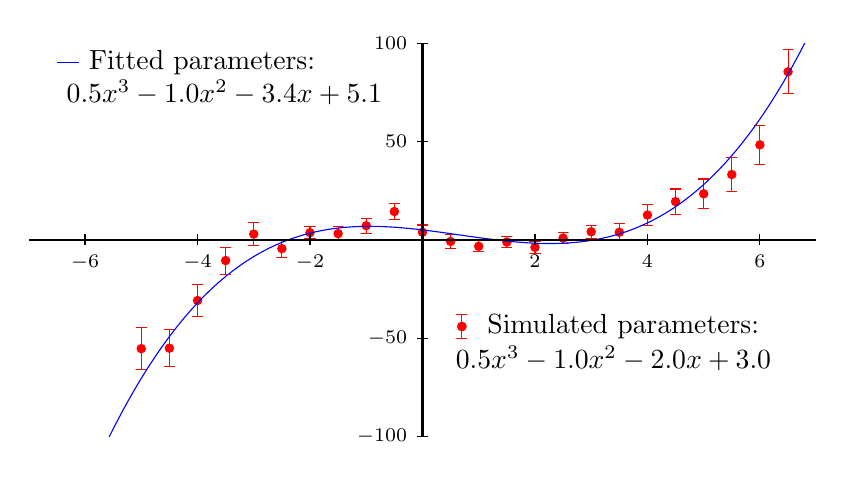
\begin{tikzpicture}
\begin{scope}[]
\pgfpathmoveto{ \pgfpointadd{\pgfpointxy {0.0} {0.0}} {\pgfpoint{0cm}{0cm}} }
\pgfpathlineto{ \pgfpointadd{\pgfpointxy {0.0} {0.0}} {\pgfpoint{10cm}{0cm}} }
\pgfpathlineto{ \pgfpointadd{\pgfpointxy {0.0} {0.0}} {\pgfpoint{10cm}{5cm}} }
\pgfpathlineto{ \pgfpointadd{\pgfpointxy {0.0} {0.0}} {\pgfpoint{0cm}{5cm}} }
\pgfpathclose
\pgfusepath{  clip, }
\begin{scope}[shift={(0.0,0.0)}]
\pgfsetxvec{\pgfpoint{0.71428573cm}{0cm}}
\pgfsetyvec{\pgfpoint{0cm}{0.025cm}}
\begin{scope}[shift={(7.0,100.0)}]
\begin{scope}[draw=red,fill=red]
\pgfpathmoveto{ \pgfpointadd{\pgfpointxy {-10.0} {-571.0535387380919}} {\pgfpoint{-2pt}{0}} }
\pgfpathlineto{ \pgfpointadd{\pgfpointxy {-10.0} {-571.0535387380919}} {\pgfpoint{2pt}{0}} }
\pgfpathlineto{ \pgfpointadd{\pgfpointxy {-10.0} {-571.0535387380919}} {\pgfpoint{0pt}{0}} }
\pgfpathlineto{ \pgfpointadd{\pgfpointxy {-10.0} {-623.095187335949}} {\pgfpoint{0pt}{0}} }
\pgfpathlineto{ \pgfpointadd{\pgfpointxy {-10.0} {-623.095187335949}} {\pgfpoint{-2pt}{0}} }
\pgfpathlineto{ \pgfpointadd{\pgfpointxy {-10.0} {-623.095187335949}} {\pgfpoint{2pt}{0}} }
\pgfusepath{ stroke, }
\node at (-10.0,-597.0743630370205) [draw=red,fill=red,circle,inner sep=0.0pt,minimum width =3.0pt,minimum height=3.0pt] {};
\end{scope}
\begin{scope}[draw=red,fill=red]
\pgfpathmoveto{ \pgfpointadd{\pgfpointxy {-9.5} {-465.4942843469761}} {\pgfpoint{-2pt}{0}} }
\pgfpathlineto{ \pgfpointadd{\pgfpointxy {-9.5} {-465.4942843469761}} {\pgfpoint{2pt}{0}} }
\pgfpathlineto{ \pgfpointadd{\pgfpointxy {-9.5} {-465.4942843469761}} {\pgfpoint{0pt}{0}} }
\pgfpathlineto{ \pgfpointadd{\pgfpointxy {-9.5} {-514.0784743698979}} {\pgfpoint{0pt}{0}} }
\pgfpathlineto{ \pgfpointadd{\pgfpointxy {-9.5} {-514.0784743698979}} {\pgfpoint{-2pt}{0}} }
\pgfpathlineto{ \pgfpointadd{\pgfpointxy {-9.5} {-514.0784743698979}} {\pgfpoint{2pt}{0}} }
\pgfusepath{ stroke, }
\node at (-9.5,-489.786379358437) [draw=red,fill=red,circle,inner sep=0.0pt,minimum width =3.0pt,minimum height=3.0pt] {};
\end{scope}
\begin{scope}[draw=red,fill=red]
\pgfpathmoveto{ \pgfpointadd{\pgfpointxy {-9.0} {-412.1044371552097}} {\pgfpoint{-2pt}{0}} }
\pgfpathlineto{ \pgfpointadd{\pgfpointxy {-9.0} {-412.1044371552097}} {\pgfpoint{2pt}{0}} }
\pgfpathlineto{ \pgfpointadd{\pgfpointxy {-9.0} {-412.1044371552097}} {\pgfpoint{0pt}{0}} }
\pgfpathlineto{ \pgfpointadd{\pgfpointxy {-9.0} {-457.3112327112828}} {\pgfpoint{0pt}{0}} }
\pgfpathlineto{ \pgfpointadd{\pgfpointxy {-9.0} {-457.3112327112828}} {\pgfpoint{-2pt}{0}} }
\pgfpathlineto{ \pgfpointadd{\pgfpointxy {-9.0} {-457.3112327112828}} {\pgfpoint{2pt}{0}} }
\pgfusepath{ stroke, }
\node at (-9.0,-434.70783493324626) [draw=red,fill=red,circle,inner sep=0.0pt,minimum width =3.0pt,minimum height=3.0pt] {};
\end{scope}
\begin{scope}[draw=red,fill=red]
\pgfpathmoveto{ \pgfpointadd{\pgfpointxy {-8.5} {-357.183759168102}} {\pgfpoint{-2pt}{0}} }
\pgfpathlineto{ \pgfpointadd{\pgfpointxy {-8.5} {-357.183759168102}} {\pgfpoint{2pt}{0}} }
\pgfpathlineto{ \pgfpointadd{\pgfpointxy {-8.5} {-357.183759168102}} {\pgfpoint{0pt}{0}} }
\pgfpathlineto{ \pgfpointadd{\pgfpointxy {-8.5} {-399.0948393426367}} {\pgfpoint{0pt}{0}} }
\pgfpathlineto{ \pgfpointadd{\pgfpointxy {-8.5} {-399.0948393426367}} {\pgfpoint{-2pt}{0}} }
\pgfpathlineto{ \pgfpointadd{\pgfpointxy {-8.5} {-399.0948393426367}} {\pgfpoint{2pt}{0}} }
\pgfusepath{ stroke, }
\node at (-8.5,-378.13929925536934) [draw=red,fill=red,circle,inner sep=0.0pt,minimum width =3.0pt,minimum height=3.0pt] {};
\end{scope}
\begin{scope}[draw=red,fill=red]
\pgfpathmoveto{ \pgfpointadd{\pgfpointxy {-8.0} {-291.87829172373085}} {\pgfpoint{-2pt}{0}} }
\pgfpathlineto{ \pgfpointadd{\pgfpointxy {-8.0} {-291.87829172373085}} {\pgfpoint{2pt}{0}} }
\pgfpathlineto{ \pgfpointadd{\pgfpointxy {-8.0} {-291.87829172373085}} {\pgfpoint{0pt}{0}} }
\pgfpathlineto{ \pgfpointadd{\pgfpointxy {-8.0} {-330.57699486952583}} {\pgfpoint{0pt}{0}} }
\pgfpathlineto{ \pgfpointadd{\pgfpointxy {-8.0} {-330.57699486952583}} {\pgfpoint{-2pt}{0}} }
\pgfpathlineto{ \pgfpointadd{\pgfpointxy {-8.0} {-330.57699486952583}} {\pgfpoint{2pt}{0}} }
\pgfusepath{ stroke, }
\node at (-8.0,-311.22764329662834) [draw=red,fill=red,circle,inner sep=0.0pt,minimum width =3.0pt,minimum height=3.0pt] {};
\end{scope}
\begin{scope}[draw=red,fill=red]
\pgfpathmoveto{ \pgfpointadd{\pgfpointxy {-7.5} {-238.3149428018001}} {\pgfpoint{-2pt}{0}} }
\pgfpathlineto{ \pgfpointadd{\pgfpointxy {-7.5} {-238.3149428018001}} {\pgfpoint{2pt}{0}} }
\pgfpathlineto{ \pgfpointadd{\pgfpointxy {-7.5} {-238.3149428018001}} {\pgfpoint{0pt}{0}} }
\pgfpathlineto{ \pgfpointadd{\pgfpointxy {-7.5} {-273.88629057157385}} {\pgfpoint{0pt}{0}} }
\pgfpathlineto{ \pgfpointadd{\pgfpointxy {-7.5} {-273.88629057157385}} {\pgfpoint{-2pt}{0}} }
\pgfpathlineto{ \pgfpointadd{\pgfpointxy {-7.5} {-273.88629057157385}} {\pgfpoint{2pt}{0}} }
\pgfusepath{ stroke, }
\node at (-7.5,-256.100616686687) [draw=red,fill=red,circle,inner sep=0.0pt,minimum width =3.0pt,minimum height=3.0pt] {};
\end{scope}
\begin{scope}[draw=red,fill=red]
\pgfpathmoveto{ \pgfpointadd{\pgfpointxy {-7.0} {-202.29808062975653}} {\pgfpoint{-2pt}{0}} }
\pgfpathlineto{ \pgfpointadd{\pgfpointxy {-7.0} {-202.29808062975653}} {\pgfpoint{2pt}{0}} }
\pgfpathlineto{ \pgfpointadd{\pgfpointxy {-7.0} {-202.29808062975653}} {\pgfpoint{0pt}{0}} }
\pgfpathlineto{ \pgfpointadd{\pgfpointxy {-7.0} {-234.82876586513075}} {\pgfpoint{0pt}{0}} }
\pgfpathlineto{ \pgfpointadd{\pgfpointxy {-7.0} {-234.82876586513075}} {\pgfpoint{-2pt}{0}} }
\pgfpathlineto{ \pgfpointadd{\pgfpointxy {-7.0} {-234.82876586513075}} {\pgfpoint{2pt}{0}} }
\pgfusepath{ stroke, }
\node at (-7.0,-218.56342324744364) [draw=red,fill=red,circle,inner sep=0.0pt,minimum width =3.0pt,minimum height=3.0pt] {};
\end{scope}
\begin{scope}[draw=red,fill=red]
\pgfpathmoveto{ \pgfpointadd{\pgfpointxy {-6.5} {-145.7322270733457}} {\pgfpoint{-2pt}{0}} }
\pgfpathlineto{ \pgfpointadd{\pgfpointxy {-6.5} {-145.7322270733457}} {\pgfpoint{2pt}{0}} }
\pgfpathlineto{ \pgfpointadd{\pgfpointxy {-6.5} {-145.7322270733457}} {\pgfpoint{0pt}{0}} }
\pgfpathlineto{ \pgfpointadd{\pgfpointxy {-6.5} {-175.31053819820306}} {\pgfpoint{0pt}{0}} }
\pgfpathlineto{ \pgfpointadd{\pgfpointxy {-6.5} {-175.31053819820306}} {\pgfpoint{-2pt}{0}} }
\pgfpathlineto{ \pgfpointadd{\pgfpointxy {-6.5} {-175.31053819820306}} {\pgfpoint{2pt}{0}} }
\pgfusepath{ stroke, }
\node at (-6.5,-160.5213826357744) [draw=red,fill=red,circle,inner sep=0.0pt,minimum width =3.0pt,minimum height=3.0pt] {};
\end{scope}
\begin{scope}[draw=red,fill=red]
\pgfpathmoveto{ \pgfpointadd{\pgfpointxy {-6.0} {-109.22115465709189}} {\pgfpoint{-2pt}{0}} }
\pgfpathlineto{ \pgfpointadd{\pgfpointxy {-6.0} {-109.22115465709189}} {\pgfpoint{2pt}{0}} }
\pgfpathlineto{ \pgfpointadd{\pgfpointxy {-6.0} {-109.22115465709189}} {\pgfpoint{0pt}{0}} }
\pgfpathlineto{ \pgfpointadd{\pgfpointxy {-6.0} {-135.93678804029298}} {\pgfpoint{0pt}{0}} }
\pgfpathlineto{ \pgfpointadd{\pgfpointxy {-6.0} {-135.93678804029298}} {\pgfpoint{-2pt}{0}} }
\pgfpathlineto{ \pgfpointadd{\pgfpointxy {-6.0} {-135.93678804029298}} {\pgfpoint{2pt}{0}} }
\pgfusepath{ stroke, }
\node at (-6.0,-122.57897134869243) [draw=red,fill=red,circle,inner sep=0.0pt,minimum width =3.0pt,minimum height=3.0pt] {};
\end{scope}
\begin{scope}[draw=red,fill=red]
\pgfpathmoveto{ \pgfpointadd{\pgfpointxy {-5.5} {-109.25232418508995}} {\pgfpoint{-2pt}{0}} }
\pgfpathlineto{ \pgfpointadd{\pgfpointxy {-5.5} {-109.25232418508995}} {\pgfpoint{2pt}{0}} }
\pgfpathlineto{ \pgfpointadd{\pgfpointxy {-5.5} {-109.25232418508995}} {\pgfpoint{0pt}{0}} }
\pgfpathlineto{ \pgfpointadd{\pgfpointxy {-5.5} {-133.19599486026908}} {\pgfpoint{0pt}{0}} }
\pgfpathlineto{ \pgfpointadd{\pgfpointxy {-5.5} {-133.19599486026908}} {\pgfpoint{-2pt}{0}} }
\pgfpathlineto{ \pgfpointadd{\pgfpointxy {-5.5} {-133.19599486026908}} {\pgfpoint{2pt}{0}} }
\pgfusepath{ stroke, }
\node at (-5.5,-121.22415952267951) [draw=red,fill=red,circle,inner sep=0.0pt,minimum width =3.0pt,minimum height=3.0pt] {};
\end{scope}
\begin{scope}[draw=red,fill=red]
\pgfpathmoveto{ \pgfpointadd{\pgfpointxy {-5.0} {-44.62018863682962}} {\pgfpoint{-2pt}{0}} }
\pgfpathlineto{ \pgfpointadd{\pgfpointxy {-5.0} {-44.62018863682962}} {\pgfpoint{2pt}{0}} }
\pgfpathlineto{ \pgfpointadd{\pgfpointxy {-5.0} {-44.62018863682962}} {\pgfpoint{0pt}{0}} }
\pgfpathlineto{ \pgfpointadd{\pgfpointxy {-5.0} {-65.88286513846168}} {\pgfpoint{0pt}{0}} }
\pgfpathlineto{ \pgfpointadd{\pgfpointxy {-5.0} {-65.88286513846168}} {\pgfpoint{-2pt}{0}} }
\pgfpathlineto{ \pgfpointadd{\pgfpointxy {-5.0} {-65.88286513846168}} {\pgfpoint{2pt}{0}} }
\pgfusepath{ stroke, }
\node at (-5.0,-55.25152688764565) [draw=red,fill=red,circle,inner sep=0.0pt,minimum width =3.0pt,minimum height=3.0pt] {};
\end{scope}
\begin{scope}[draw=red,fill=red]
\pgfpathmoveto{ \pgfpointadd{\pgfpointxy {-4.5} {-45.66786522760035}} {\pgfpoint{-2pt}{0}} }
\pgfpathlineto{ \pgfpointadd{\pgfpointxy {-4.5} {-45.66786522760035}} {\pgfpoint{2pt}{0}} }
\pgfpathlineto{ \pgfpointadd{\pgfpointxy {-4.5} {-45.66786522760035}} {\pgfpoint{0pt}{0}} }
\pgfpathlineto{ \pgfpointadd{\pgfpointxy {-4.5} {-64.33926597872156}} {\pgfpoint{0pt}{0}} }
\pgfpathlineto{ \pgfpointadd{\pgfpointxy {-4.5} {-64.33926597872156}} {\pgfpoint{-2pt}{0}} }
\pgfpathlineto{ \pgfpointadd{\pgfpointxy {-4.5} {-64.33926597872156}} {\pgfpoint{2pt}{0}} }
\pgfusepath{ stroke, }
\node at (-4.5,-55.00356560316096) [draw=red,fill=red,circle,inner sep=0.0pt,minimum width =3.0pt,minimum height=3.0pt] {};
\end{scope}
\begin{scope}[draw=red,fill=red]
\pgfpathmoveto{ \pgfpointadd{\pgfpointxy {-4.0} {-22.71518997590085}} {\pgfpoint{-2pt}{0}} }
\pgfpathlineto{ \pgfpointadd{\pgfpointxy {-4.0} {-22.71518997590085}} {\pgfpoint{2pt}{0}} }
\pgfpathlineto{ \pgfpointadd{\pgfpointxy {-4.0} {-22.71518997590085}} {\pgfpoint{0pt}{0}} }
\pgfpathlineto{ \pgfpointadd{\pgfpointxy {-4.0} {-38.880715036497286}} {\pgfpoint{0pt}{0}} }
\pgfpathlineto{ \pgfpointadd{\pgfpointxy {-4.0} {-38.880715036497286}} {\pgfpoint{-2pt}{0}} }
\pgfpathlineto{ \pgfpointadd{\pgfpointxy {-4.0} {-38.880715036497286}} {\pgfpoint{2pt}{0}} }
\pgfusepath{ stroke, }
\node at (-4.0,-30.797952506199067) [draw=red,fill=red,circle,inner sep=0.0pt,minimum width =3.0pt,minimum height=3.0pt] {};
\end{scope}
\begin{scope}[draw=red,fill=red]
\pgfpathmoveto{ \pgfpointadd{\pgfpointxy {-3.5} {-3.623367622026165}} {\pgfpoint{-2pt}{0}} }
\pgfpathlineto{ \pgfpointadd{\pgfpointxy {-3.5} {-3.623367622026165}} {\pgfpoint{2pt}{0}} }
\pgfpathlineto{ \pgfpointadd{\pgfpointxy {-3.5} {-3.623367622026165}} {\pgfpoint{0pt}{0}} }
\pgfpathlineto{ \pgfpointadd{\pgfpointxy {-3.5} {-17.357328788992056}} {\pgfpoint{0pt}{0}} }
\pgfpathlineto{ \pgfpointadd{\pgfpointxy {-3.5} {-17.357328788992056}} {\pgfpoint{-2pt}{0}} }
\pgfpathlineto{ \pgfpointadd{\pgfpointxy {-3.5} {-17.357328788992056}} {\pgfpoint{2pt}{0}} }
\pgfusepath{ stroke, }
\node at (-3.5,-10.490348205509111) [draw=red,fill=red,circle,inner sep=0.0pt,minimum width =3.0pt,minimum height=3.0pt] {};
\end{scope}
\begin{scope}[draw=red,fill=red]
\pgfpathmoveto{ \pgfpointadd{\pgfpointxy {-3.0} {8.659705441078653}} {\pgfpoint{-2pt}{0}} }
\pgfpathlineto{ \pgfpointadd{\pgfpointxy {-3.0} {8.659705441078653}} {\pgfpoint{2pt}{0}} }
\pgfpathlineto{ \pgfpointadd{\pgfpointxy {-3.0} {8.659705441078653}} {\pgfpoint{0pt}{0}} }
\pgfpathlineto{ \pgfpointadd{\pgfpointxy {-3.0} {-2.688763787270882}} {\pgfpoint{0pt}{0}} }
\pgfpathlineto{ \pgfpointadd{\pgfpointxy {-3.0} {-2.688763787270882}} {\pgfpoint{-2pt}{0}} }
\pgfpathlineto{ \pgfpointadd{\pgfpointxy {-3.0} {-2.688763787270882}} {\pgfpoint{2pt}{0}} }
\pgfusepath{ stroke, }
\node at (-3.0,2.985470826903885) [draw=red,fill=red,circle,inner sep=0.0pt,minimum width =3.0pt,minimum height=3.0pt] {};
\end{scope}
\begin{scope}[draw=red,fill=red]
\pgfpathmoveto{ \pgfpointadd{\pgfpointxy {-2.5} {0.03452070884278502}} {\pgfpoint{-2pt}{0}} }
\pgfpathlineto{ \pgfpointadd{\pgfpointxy {-2.5} {0.03452070884278502}} {\pgfpoint{2pt}{0}} }
\pgfpathlineto{ \pgfpointadd{\pgfpointxy {-2.5} {0.03452070884278502}} {\pgfpoint{0pt}{0}} }
\pgfpathlineto{ \pgfpointadd{\pgfpointxy {-2.5} {-8.889908192055266}} {\pgfpoint{0pt}{0}} }
\pgfpathlineto{ \pgfpointadd{\pgfpointxy {-2.5} {-8.889908192055266}} {\pgfpoint{-2pt}{0}} }
\pgfpathlineto{ \pgfpointadd{\pgfpointxy {-2.5} {-8.889908192055266}} {\pgfpoint{2pt}{0}} }
\pgfusepath{ stroke, }
\node at (-2.5,-4.427693741606241) [draw=red,fill=red,circle,inner sep=0.0pt,minimum width =3.0pt,minimum height=3.0pt] {};
\end{scope}
\begin{scope}[draw=red,fill=red]
\pgfpathmoveto{ \pgfpointadd{\pgfpointxy {-2.0} {6.691469768324479}} {\pgfpoint{-2pt}{0}} }
\pgfpathlineto{ \pgfpointadd{\pgfpointxy {-2.0} {6.691469768324479}} {\pgfpoint{2pt}{0}} }
\pgfpathlineto{ \pgfpointadd{\pgfpointxy {-2.0} {6.691469768324479}} {\pgfpoint{0pt}{0}} }
\pgfpathlineto{ \pgfpointadd{\pgfpointxy {-2.0} {0.6914697683244793}} {\pgfpoint{0pt}{0}} }
\pgfpathlineto{ \pgfpointadd{\pgfpointxy {-2.0} {0.6914697683244793}} {\pgfpoint{-2pt}{0}} }
\pgfpathlineto{ \pgfpointadd{\pgfpointxy {-2.0} {0.6914697683244793}} {\pgfpoint{2pt}{0}} }
\pgfusepath{ stroke, }
\node at (-2.0,3.6914697683244793) [draw=red,fill=red,circle,inner sep=0.0pt,minimum width =3.0pt,minimum height=3.0pt] {};
\end{scope}
\begin{scope}[draw=red,fill=red]
\pgfpathmoveto{ \pgfpointadd{\pgfpointxy {-1.5} {6.642849316210677}} {\pgfpoint{-2pt}{0}} }
\pgfpathlineto{ \pgfpointadd{\pgfpointxy {-1.5} {6.642849316210677}} {\pgfpoint{2pt}{0}} }
\pgfpathlineto{ \pgfpointadd{\pgfpointxy {-1.5} {6.642849316210677}} {\pgfpoint{0pt}{0}} }
\pgfpathlineto{ \pgfpointadd{\pgfpointxy {-1.5} {-0.2294320070583371}} {\pgfpoint{0pt}{0}} }
\pgfpathlineto{ \pgfpointadd{\pgfpointxy {-1.5} {-0.2294320070583371}} {\pgfpoint{-2pt}{0}} }
\pgfpathlineto{ \pgfpointadd{\pgfpointxy {-1.5} {-0.2294320070583371}} {\pgfpoint{2pt}{0}} }
\pgfusepath{ stroke, }
\node at (-1.5,3.20670865457617) [draw=red,fill=red,circle,inner sep=0.0pt,minimum width =3.0pt,minimum height=3.0pt] {};
\end{scope}
\begin{scope}[draw=red,fill=red]
\pgfpathmoveto{ \pgfpointadd{\pgfpointxy {-1.0} {11.107898214064939}} {\pgfpoint{-2pt}{0}} }
\pgfpathlineto{ \pgfpointadd{\pgfpointxy {-1.0} {11.107898214064939}} {\pgfpoint{2pt}{0}} }
\pgfpathlineto{ \pgfpointadd{\pgfpointxy {-1.0} {11.107898214064939}} {\pgfpoint{0pt}{0}} }
\pgfpathlineto{ \pgfpointadd{\pgfpointxy {-1.0} {3.3662408272909987}} {\pgfpoint{0pt}{0}} }
\pgfpathlineto{ \pgfpointadd{\pgfpointxy {-1.0} {3.3662408272909987}} {\pgfpoint{-2pt}{0}} }
\pgfpathlineto{ \pgfpointadd{\pgfpointxy {-1.0} {3.3662408272909987}} {\pgfpoint{2pt}{0}} }
\pgfusepath{ stroke, }
\node at (-1.0,7.237069520677969) [draw=red,fill=red,circle,inner sep=0.0pt,minimum width =3.0pt,minimum height=3.0pt] {};
\end{scope}
\begin{scope}[draw=red,fill=red]
\pgfpathmoveto{ \pgfpointadd{\pgfpointxy {-0.5} {18.362804815403905}} {\pgfpoint{-2pt}{0}} }
\pgfpathlineto{ \pgfpointadd{\pgfpointxy {-0.5} {18.362804815403905}} {\pgfpoint{2pt}{0}} }
\pgfpathlineto{ \pgfpointadd{\pgfpointxy {-0.5} {18.362804815403905}} {\pgfpoint{0pt}{0}} }
\pgfpathlineto{ \pgfpointadd{\pgfpointxy {-0.5} {10.522231941469602}} {\pgfpoint{0pt}{0}} }
\pgfpathlineto{ \pgfpointadd{\pgfpointxy {-0.5} {10.522231941469602}} {\pgfpoint{-2pt}{0}} }
\pgfpathlineto{ \pgfpointadd{\pgfpointxy {-0.5} {10.522231941469602}} {\pgfpoint{2pt}{0}} }
\pgfusepath{ stroke, }
\node at (-0.5,14.442518378436754) [draw=red,fill=red,circle,inner sep=0.0pt,minimum width =3.0pt,minimum height=3.0pt] {};
\end{scope}
\begin{scope}[draw=red,fill=red]
\pgfpathmoveto{ \pgfpointadd{\pgfpointxy {0.0} {7.612007955975413}} {\pgfpoint{-2pt}{0}} }
\pgfpathlineto{ \pgfpointadd{\pgfpointxy {0.0} {7.612007955975413}} {\pgfpoint{2pt}{0}} }
\pgfpathlineto{ \pgfpointadd{\pgfpointxy {0.0} {7.612007955975413}} {\pgfpoint{0pt}{0}} }
\pgfpathlineto{ \pgfpointadd{\pgfpointxy {0.0} {0.14790634083765797}} {\pgfpoint{0pt}{0}} }
\pgfpathlineto{ \pgfpointadd{\pgfpointxy {0.0} {0.14790634083765797}} {\pgfpoint{-2pt}{0}} }
\pgfpathlineto{ \pgfpointadd{\pgfpointxy {0.0} {0.14790634083765797}} {\pgfpoint{2pt}{0}} }
\pgfusepath{ stroke, }
\node at (0.0,3.879957148406535) [draw=red,fill=red,circle,inner sep=0.0pt,minimum width =3.0pt,minimum height=3.0pt] {};
\end{scope}
\begin{scope}[draw=red,fill=red]
\pgfpathmoveto{ \pgfpointadd{\pgfpointxy {0.5} {2.5683907793851475}} {\pgfpoint{-2pt}{0}} }
\pgfpathlineto{ \pgfpointadd{\pgfpointxy {0.5} {2.5683907793851475}} {\pgfpoint{2pt}{0}} }
\pgfpathlineto{ \pgfpointadd{\pgfpointxy {0.5} {2.5683907793851475}} {\pgfpoint{0pt}{0}} }
\pgfpathlineto{ \pgfpointadd{\pgfpointxy {0.5} {-4.124191624182105}} {\pgfpoint{0pt}{0}} }
\pgfpathlineto{ \pgfpointadd{\pgfpointxy {0.5} {-4.124191624182105}} {\pgfpoint{-2pt}{0}} }
\pgfpathlineto{ \pgfpointadd{\pgfpointxy {0.5} {-4.124191624182105}} {\pgfpoint{2pt}{0}} }
\pgfusepath{ stroke, }
\node at (0.5,-0.7779004223984787) [draw=red,fill=red,circle,inner sep=0.0pt,minimum width =3.0pt,minimum height=3.0pt] {};
\end{scope}
\begin{scope}[draw=red,fill=red]
\pgfpathmoveto{ \pgfpointadd{\pgfpointxy {1.0} {-0.5092360123617312}} {\pgfpoint{-2pt}{0}} }
\pgfpathlineto{ \pgfpointadd{\pgfpointxy {1.0} {-0.5092360123617312}} {\pgfpoint{2pt}{0}} }
\pgfpathlineto{ \pgfpointadd{\pgfpointxy {1.0} {-0.5092360123617312}} {\pgfpoint{0pt}{0}} }
\pgfpathlineto{ \pgfpointadd{\pgfpointxy {1.0} {-5.923449574734827}} {\pgfpoint{0pt}{0}} }
\pgfpathlineto{ \pgfpointadd{\pgfpointxy {1.0} {-5.923449574734827}} {\pgfpoint{-2pt}{0}} }
\pgfpathlineto{ \pgfpointadd{\pgfpointxy {1.0} {-5.923449574734827}} {\pgfpoint{2pt}{0}} }
\pgfusepath{ stroke, }
\node at (1.0,-3.2163427935482787) [draw=red,fill=red,circle,inner sep=0.0pt,minimum width =3.0pt,minimum height=3.0pt] {};
\end{scope}
\begin{scope}[draw=red,fill=red]
\pgfpathmoveto{ \pgfpointadd{\pgfpointxy {1.5} {1.6701722960789132}} {\pgfpoint{-2pt}{0}} }
\pgfpathlineto{ \pgfpointadd{\pgfpointxy {1.5} {1.6701722960789132}} {\pgfpoint{2pt}{0}} }
\pgfpathlineto{ \pgfpointadd{\pgfpointxy {1.5} {1.6701722960789132}} {\pgfpoint{0pt}{0}} }
\pgfpathlineto{ \pgfpointadd{\pgfpointxy {1.5} {-3.8298277039210866}} {\pgfpoint{0pt}{0}} }
\pgfpathlineto{ \pgfpointadd{\pgfpointxy {1.5} {-3.8298277039210866}} {\pgfpoint{-2pt}{0}} }
\pgfpathlineto{ \pgfpointadd{\pgfpointxy {1.5} {-3.8298277039210866}} {\pgfpoint{2pt}{0}} }
\pgfusepath{ stroke, }
\node at (1.5,-1.0798277039210868) [draw=red,fill=red,circle,inner sep=0.0pt,minimum width =3.0pt,minimum height=3.0pt] {};
\end{scope}
\begin{scope}[draw=red,fill=red]
\pgfpathmoveto{ \pgfpointadd{\pgfpointxy {2.0} {-0.7755617046804377}} {\pgfpoint{-2pt}{0}} }
\pgfpathlineto{ \pgfpointadd{\pgfpointxy {2.0} {-0.7755617046804377}} {\pgfpoint{2pt}{0}} }
\pgfpathlineto{ \pgfpointadd{\pgfpointxy {2.0} {-0.7755617046804377}} {\pgfpoint{0pt}{0}} }
\pgfpathlineto{ \pgfpointadd{\pgfpointxy {2.0} {-6.775561704680438}} {\pgfpoint{0pt}{0}} }
\pgfpathlineto{ \pgfpointadd{\pgfpointxy {2.0} {-6.775561704680438}} {\pgfpoint{-2pt}{0}} }
\pgfpathlineto{ \pgfpointadd{\pgfpointxy {2.0} {-6.775561704680438}} {\pgfpoint{2pt}{0}} }
\pgfusepath{ stroke, }
\node at (2.0,-3.7755617046804377) [draw=red,fill=red,circle,inner sep=0.0pt,minimum width =3.0pt,minimum height=3.0pt] {};
\end{scope}
\begin{scope}[draw=red,fill=red]
\pgfpathmoveto{ \pgfpointadd{\pgfpointxy {2.5} {3.599233927702615}} {\pgfpoint{-2pt}{0}} }
\pgfpathlineto{ \pgfpointadd{\pgfpointxy {2.5} {3.599233927702615}} {\pgfpoint{2pt}{0}} }
\pgfpathlineto{ \pgfpointadd{\pgfpointxy {2.5} {3.599233927702615}} {\pgfpoint{0pt}{0}} }
\pgfpathlineto{ \pgfpointadd{\pgfpointxy {2.5} {-1.72364172782968}} {\pgfpoint{0pt}{0}} }
\pgfpathlineto{ \pgfpointadd{\pgfpointxy {2.5} {-1.72364172782968}} {\pgfpoint{-2pt}{0}} }
\pgfpathlineto{ \pgfpointadd{\pgfpointxy {2.5} {-1.72364172782968}} {\pgfpoint{2pt}{0}} }
\pgfusepath{ stroke, }
\node at (2.5,0.9377960999364674) [draw=red,fill=red,circle,inner sep=0.0pt,minimum width =3.0pt,minimum height=3.0pt] {};
\end{scope}
\begin{scope}[draw=red,fill=red]
\pgfpathmoveto{ \pgfpointadd{\pgfpointxy {3.0} {7.3753525624062775}} {\pgfpoint{-2pt}{0}} }
\pgfpathlineto{ \pgfpointadd{\pgfpointxy {3.0} {7.3753525624062775}} {\pgfpoint{2pt}{0}} }
\pgfpathlineto{ \pgfpointadd{\pgfpointxy {3.0} {7.3753525624062775}} {\pgfpoint{0pt}{0}} }
\pgfpathlineto{ \pgfpointadd{\pgfpointxy {3.0} {0.9258628196231}} {\pgfpoint{0pt}{0}} }
\pgfpathlineto{ \pgfpointadd{\pgfpointxy {3.0} {0.9258628196231}} {\pgfpoint{-2pt}{0}} }
\pgfpathlineto{ \pgfpointadd{\pgfpointxy {3.0} {0.9258628196231}} {\pgfpoint{2pt}{0}} }
\pgfusepath{ stroke, }
\node at (3.0,4.150607691014689) [draw=red,fill=red,circle,inner sep=0.0pt,minimum width =3.0pt,minimum height=3.0pt] {};
\end{scope}
\begin{scope}[draw=red,fill=red]
\pgfpathmoveto{ \pgfpointadd{\pgfpointxy {3.5} {8.180402037547292}} {\pgfpoint{-2pt}{0}} }
\pgfpathlineto{ \pgfpointadd{\pgfpointxy {3.5} {8.180402037547292}} {\pgfpoint{2pt}{0}} }
\pgfpathlineto{ \pgfpointadd{\pgfpointxy {3.5} {8.180402037547292}} {\pgfpoint{0pt}{0}} }
\pgfpathlineto{ \pgfpointadd{\pgfpointxy {3.5} {-0.37481475202485726}} {\pgfpoint{0pt}{0}} }
\pgfpathlineto{ \pgfpointadd{\pgfpointxy {3.5} {-0.37481475202485726}} {\pgfpoint{-2pt}{0}} }
\pgfpathlineto{ \pgfpointadd{\pgfpointxy {3.5} {-0.37481475202485726}} {\pgfpoint{2pt}{0}} }
\pgfusepath{ stroke, }
\node at (3.5,3.9027936427612175) [draw=red,fill=red,circle,inner sep=0.0pt,minimum width =3.0pt,minimum height=3.0pt] {};
\end{scope}
\begin{scope}[draw=red,fill=red]
\pgfpathmoveto{ \pgfpointadd{\pgfpointxy {4.0} {17.985284457749778}} {\pgfpoint{-2pt}{0}} }
\pgfpathlineto{ \pgfpointadd{\pgfpointxy {4.0} {17.985284457749778}} {\pgfpoint{2pt}{0}} }
\pgfpathlineto{ \pgfpointadd{\pgfpointxy {4.0} {17.985284457749778}} {\pgfpoint{0pt}{0}} }
\pgfpathlineto{ \pgfpointadd{\pgfpointxy {4.0} {7.352034877038976}} {\pgfpoint{0pt}{0}} }
\pgfpathlineto{ \pgfpointadd{\pgfpointxy {4.0} {7.352034877038976}} {\pgfpoint{-2pt}{0}} }
\pgfpathlineto{ \pgfpointadd{\pgfpointxy {4.0} {7.352034877038976}} {\pgfpoint{2pt}{0}} }
\pgfusepath{ stroke, }
\node at (4.0,12.668659667394376) [draw=red,fill=red,circle,inner sep=0.0pt,minimum width =3.0pt,minimum height=3.0pt] {};
\end{scope}
\begin{scope}[draw=red,fill=red]
\pgfpathmoveto{ \pgfpointadd{\pgfpointxy {4.5} {25.865344976413038}} {\pgfpoint{-2pt}{0}} }
\pgfpathlineto{ \pgfpointadd{\pgfpointxy {4.5} {25.865344976413038}} {\pgfpoint{2pt}{0}} }
\pgfpathlineto{ \pgfpointadd{\pgfpointxy {4.5} {25.865344976413038}} {\pgfpoint{0pt}{0}} }
\pgfpathlineto{ \pgfpointadd{\pgfpointxy {4.5} {13.076147060789562}} {\pgfpoint{0pt}{0}} }
\pgfpathlineto{ \pgfpointadd{\pgfpointxy {4.5} {13.076147060789562}} {\pgfpoint{-2pt}{0}} }
\pgfpathlineto{ \pgfpointadd{\pgfpointxy {4.5} {13.076147060789562}} {\pgfpoint{2pt}{0}} }
\pgfusepath{ stroke, }
\node at (4.5,19.4707460186013) [draw=red,fill=red,circle,inner sep=0.0pt,minimum width =3.0pt,minimum height=3.0pt] {};
\end{scope}
\begin{scope}[draw=red,fill=red]
\pgfpathmoveto{ \pgfpointadd{\pgfpointxy {5.0} {30.966184447206345}} {\pgfpoint{-2pt}{0}} }
\pgfpathlineto{ \pgfpointadd{\pgfpointxy {5.0} {30.966184447206345}} {\pgfpoint{2pt}{0}} }
\pgfpathlineto{ \pgfpointadd{\pgfpointxy {5.0} {30.966184447206345}} {\pgfpoint{0pt}{0}} }
\pgfpathlineto{ \pgfpointadd{\pgfpointxy {5.0} {15.920823430019084}} {\pgfpoint{0pt}{0}} }
\pgfpathlineto{ \pgfpointadd{\pgfpointxy {5.0} {15.920823430019084}} {\pgfpoint{-2pt}{0}} }
\pgfpathlineto{ \pgfpointadd{\pgfpointxy {5.0} {15.920823430019084}} {\pgfpoint{2pt}{0}} }
\pgfusepath{ stroke, }
\node at (5.0,23.443503938612714) [draw=red,fill=red,circle,inner sep=0.0pt,minimum width =3.0pt,minimum height=3.0pt] {};
\end{scope}
\begin{scope}[draw=red,fill=red]
\pgfpathmoveto{ \pgfpointadd{\pgfpointxy {5.5} {41.93279338298936}} {\pgfpoint{-2pt}{0}} }
\pgfpathlineto{ \pgfpointadd{\pgfpointxy {5.5} {41.93279338298936}} {\pgfpoint{2pt}{0}} }
\pgfpathlineto{ \pgfpointadd{\pgfpointxy {5.5} {41.93279338298936}} {\pgfpoint{0pt}{0}} }
\pgfpathlineto{ \pgfpointadd{\pgfpointxy {5.5} {24.52570570519744}} {\pgfpoint{0pt}{0}} }
\pgfpathlineto{ \pgfpointadd{\pgfpointxy {5.5} {24.52570570519744}} {\pgfpoint{-2pt}{0}} }
\pgfpathlineto{ \pgfpointadd{\pgfpointxy {5.5} {24.52570570519744}} {\pgfpoint{2pt}{0}} }
\pgfusepath{ stroke, }
\node at (5.5,33.2292495440934) [draw=red,fill=red,circle,inner sep=0.0pt,minimum width =3.0pt,minimum height=3.0pt] {};
\end{scope}
\begin{scope}[draw=red,fill=red]
\pgfpathmoveto{ \pgfpointadd{\pgfpointxy {6.0} {58.24963967593858}} {\pgfpoint{-2pt}{0}} }
\pgfpathlineto{ \pgfpointadd{\pgfpointxy {6.0} {58.24963967593858}} {\pgfpoint{2pt}{0}} }
\pgfpathlineto{ \pgfpointadd{\pgfpointxy {6.0} {58.24963967593858}} {\pgfpoint{0pt}{0}} }
\pgfpathlineto{ \pgfpointadd{\pgfpointxy {6.0} {38.375131809551036}} {\pgfpoint{0pt}{0}} }
\pgfpathlineto{ \pgfpointadd{\pgfpointxy {6.0} {38.375131809551036}} {\pgfpoint{-2pt}{0}} }
\pgfpathlineto{ \pgfpointadd{\pgfpointxy {6.0} {38.375131809551036}} {\pgfpoint{2pt}{0}} }
\pgfusepath{ stroke, }
\node at (6.0,48.31238574274481) [draw=red,fill=red,circle,inner sep=0.0pt,minimum width =3.0pt,minimum height=3.0pt] {};
\end{scope}
\begin{scope}[draw=red,fill=red]
\pgfpathmoveto{ \pgfpointadd{\pgfpointxy {6.5} {96.67541812918063}} {\pgfpoint{-2pt}{0}} }
\pgfpathlineto{ \pgfpointadd{\pgfpointxy {6.5} {96.67541812918063}} {\pgfpoint{2pt}{0}} }
\pgfpathlineto{ \pgfpointadd{\pgfpointxy {6.5} {96.67541812918063}} {\pgfpoint{0pt}{0}} }
\pgfpathlineto{ \pgfpointadd{\pgfpointxy {6.5} {74.22955138348391}} {\pgfpoint{0pt}{0}} }
\pgfpathlineto{ \pgfpointadd{\pgfpointxy {6.5} {74.22955138348391}} {\pgfpoint{-2pt}{0}} }
\pgfpathlineto{ \pgfpointadd{\pgfpointxy {6.5} {74.22955138348391}} {\pgfpoint{2pt}{0}} }
\pgfusepath{ stroke, }
\node at (6.5,85.45248475633227) [draw=red,fill=red,circle,inner sep=0.0pt,minimum width =3.0pt,minimum height=3.0pt] {};
\end{scope}
\begin{scope}[draw=red,fill=red]
\pgfpathmoveto{ \pgfpointadd{\pgfpointxy {7.0} {150.98758050732656}} {\pgfpoint{-2pt}{0}} }
\pgfpathlineto{ \pgfpointadd{\pgfpointxy {7.0} {150.98758050732656}} {\pgfpoint{2pt}{0}} }
\pgfpathlineto{ \pgfpointadd{\pgfpointxy {7.0} {150.98758050732656}} {\pgfpoint{0pt}{0}} }
\pgfpathlineto{ \pgfpointadd{\pgfpointxy {7.0} {125.86886842538368}} {\pgfpoint{0pt}{0}} }
\pgfpathlineto{ \pgfpointadd{\pgfpointxy {7.0} {125.86886842538368}} {\pgfpoint{-2pt}{0}} }
\pgfpathlineto{ \pgfpointadd{\pgfpointxy {7.0} {125.86886842538368}} {\pgfpoint{2pt}{0}} }
\pgfusepath{ stroke, }
\node at (7.0,138.42822446635512) [draw=red,fill=red,circle,inner sep=0.0pt,minimum width =3.0pt,minimum height=3.0pt] {};
\end{scope}
\begin{scope}[draw=red,fill=red]
\pgfpathmoveto{ \pgfpointadd{\pgfpointxy {7.5} {137.62912541707732}} {\pgfpoint{-2pt}{0}} }
\pgfpathlineto{ \pgfpointadd{\pgfpointxy {7.5} {137.62912541707732}} {\pgfpoint{2pt}{0}} }
\pgfpathlineto{ \pgfpointadd{\pgfpointxy {7.5} {137.62912541707732}} {\pgfpoint{0pt}{0}} }
\pgfpathlineto{ \pgfpointadd{\pgfpointxy {7.5} {109.73875078627674}} {\pgfpoint{0pt}{0}} }
\pgfpathlineto{ \pgfpointadd{\pgfpointxy {7.5} {109.73875078627674}} {\pgfpoint{-2pt}{0}} }
\pgfpathlineto{ \pgfpointadd{\pgfpointxy {7.5} {109.73875078627674}} {\pgfpoint{2pt}{0}} }
\pgfusepath{ stroke, }
\node at (7.5,123.68393810167703) [draw=red,fill=red,circle,inner sep=0.0pt,minimum width =3.0pt,minimum height=3.0pt] {};
\end{scope}
\begin{scope}[draw=red,fill=red]
\pgfpathmoveto{ \pgfpointadd{\pgfpointxy {8.0} {201.411347251231}} {\pgfpoint{-2pt}{0}} }
\pgfpathlineto{ \pgfpointadd{\pgfpointxy {8.0} {201.411347251231}} {\pgfpoint{2pt}{0}} }
\pgfpathlineto{ \pgfpointadd{\pgfpointxy {8.0} {201.411347251231}} {\pgfpoint{0pt}{0}} }
\pgfpathlineto{ \pgfpointadd{\pgfpointxy {8.0} {170.65317093071172}} {\pgfpoint{0pt}{0}} }
\pgfpathlineto{ \pgfpointadd{\pgfpointxy {8.0} {170.65317093071172}} {\pgfpoint{-2pt}{0}} }
\pgfpathlineto{ \pgfpointadd{\pgfpointxy {8.0} {170.65317093071172}} {\pgfpoint{2pt}{0}} }
\pgfusepath{ stroke, }
\node at (8.0,186.03225909097137) [draw=red,fill=red,circle,inner sep=0.0pt,minimum width =3.0pt,minimum height=3.0pt] {};
\end{scope}
\begin{scope}[draw=red,fill=red]
\pgfpathmoveto{ \pgfpointadd{\pgfpointxy {8.5} {240.7691872656242}} {\pgfpoint{-2pt}{0}} }
\pgfpathlineto{ \pgfpointadd{\pgfpointxy {8.5} {240.7691872656242}} {\pgfpoint{2pt}{0}} }
\pgfpathlineto{ \pgfpointadd{\pgfpointxy {8.5} {240.7691872656242}} {\pgfpoint{0pt}{0}} }
\pgfpathlineto{ \pgfpointadd{\pgfpointxy {8.5} {207.04966506219702}} {\pgfpoint{0pt}{0}} }
\pgfpathlineto{ \pgfpointadd{\pgfpointxy {8.5} {207.04966506219702}} {\pgfpoint{-2pt}{0}} }
\pgfpathlineto{ \pgfpointadd{\pgfpointxy {8.5} {207.04966506219702}} {\pgfpoint{2pt}{0}} }
\pgfusepath{ stroke, }
\node at (8.5,223.9094261639106) [draw=red,fill=red,circle,inner sep=0.0pt,minimum width =3.0pt,minimum height=3.0pt] {};
\end{scope}
\begin{scope}[draw=red,fill=red]
\pgfpathmoveto{ \pgfpointadd{\pgfpointxy {9.0} {309.16018045080494}} {\pgfpoint{-2pt}{0}} }
\pgfpathlineto{ \pgfpointadd{\pgfpointxy {9.0} {309.16018045080494}} {\pgfpoint{2pt}{0}} }
\pgfpathlineto{ \pgfpointadd{\pgfpointxy {9.0} {309.16018045080494}} {\pgfpoint{0pt}{0}} }
\pgfpathlineto{ \pgfpointadd{\pgfpointxy {9.0} {272.3882412344571}} {\pgfpoint{0pt}{0}} }
\pgfpathlineto{ \pgfpointadd{\pgfpointxy {9.0} {272.3882412344571}} {\pgfpoint{-2pt}{0}} }
\pgfpathlineto{ \pgfpointadd{\pgfpointxy {9.0} {272.3882412344571}} {\pgfpoint{2pt}{0}} }
\pgfusepath{ stroke, }
\node at (9.0,290.774210842631) [draw=red,fill=red,circle,inner sep=0.0pt,minimum width =3.0pt,minimum height=3.0pt] {};
\end{scope}
\begin{scope}[draw=red,fill=red]
\pgfpathmoveto{ \pgfpointadd{\pgfpointxy {9.5} {335.072764831252}} {\pgfpoint{-2pt}{0}} }
\pgfpathlineto{ \pgfpointadd{\pgfpointxy {9.5} {335.072764831252}} {\pgfpoint{2pt}{0}} }
\pgfpathlineto{ \pgfpointadd{\pgfpointxy {9.5} {335.072764831252}} {\pgfpoint{0pt}{0}} }
\pgfpathlineto{ \pgfpointadd{\pgfpointxy {9.5} {295.159675295541}} {\pgfpoint{0pt}{0}} }
\pgfpathlineto{ \pgfpointadd{\pgfpointxy {9.5} {295.159675295541}} {\pgfpoint{-2pt}{0}} }
\pgfpathlineto{ \pgfpointadd{\pgfpointxy {9.5} {295.159675295541}} {\pgfpoint{2pt}{0}} }
\pgfusepath{ stroke, }
\node at (9.5,315.1162200633965) [draw=red,fill=red,circle,inner sep=0.0pt,minimum width =3.0pt,minimum height=3.0pt] {};
\end{scope}
\begin{scope}[draw=red,fill=red]
\pgfpathmoveto{ \pgfpointadd{\pgfpointxy {10.0} {419.00919636744237}} {\pgfpoint{-2pt}{0}} }
\pgfpathlineto{ \pgfpointadd{\pgfpointxy {10.0} {419.00919636744237}} {\pgfpoint{2pt}{0}} }
\pgfpathlineto{ \pgfpointadd{\pgfpointxy {10.0} {419.00919636744237}} {\pgfpoint{0pt}{0}} }
\pgfpathlineto{ \pgfpointadd{\pgfpointxy {10.0} {375.86842478588056}} {\pgfpoint{0pt}{0}} }
\pgfpathlineto{ \pgfpointadd{\pgfpointxy {10.0} {375.86842478588056}} {\pgfpoint{-2pt}{0}} }
\pgfpathlineto{ \pgfpointadd{\pgfpointxy {10.0} {375.86842478588056}} {\pgfpoint{2pt}{0}} }
\pgfusepath{ stroke, }
\node at (10.0,397.43881057666147) [draw=red,fill=red,circle,inner sep=0.0pt,minimum width =3.0pt,minimum height=3.0pt] {};
\end{scope}
\end{scope}
\pgfsetxvec{\pgfpoint{1cm}{0cm}}
\pgfsetyvec{\pgfpoint{0cm}{1cm}}
\end{scope}
\end{scope}
\begin{scope}[draw=red,fill=red]
\pgfpathmoveto{ \pgfpointadd{\pgfpointxy {5.5} {1.55}} {\pgfpoint{-2pt}{0}} }
\pgfpathlineto{ \pgfpointadd{\pgfpointxy {5.5} {1.55}} {\pgfpoint{2pt}{0}} }
\pgfpathlineto{ \pgfpointadd{\pgfpointxy {5.5} {1.55}} {\pgfpoint{0pt}{0}} }
\pgfpathlineto{ \pgfpointadd{\pgfpointxy {5.5} {1.25}} {\pgfpoint{0pt}{0}} }
\pgfpathlineto{ \pgfpointadd{\pgfpointxy {5.5} {1.25}} {\pgfpoint{-2pt}{0}} }
\pgfpathlineto{ \pgfpointadd{\pgfpointxy {5.5} {1.25}} {\pgfpoint{2pt}{0}} }
\pgfusepath{ stroke, }
\node at (5.5,1.4) [draw=red,fill=red,circle,inner sep=0.0pt,minimum width =3.0pt,minimum height=3.0pt] {};
\end{scope}
\node at (5.5,1.4) [draw=red,fill=red,circle,inner sep=0.0pt,minimum width =3.0pt,minimum height=3.0pt] {};
\node at (5.7000003,1.4) [right,,] {Simulated parameters:};
\node at (5.3,1.0) [right,] {$0.5x^3 -1.0x^2 -2.0x +3.0$};
\begin{scope}[shift={(0.0,0.0)}]
\pgfsetxvec{\pgfpoint{0.71428573cm}{0cm}}
\pgfsetyvec{\pgfpoint{0cm}{0.025cm}}
\begin{scope}[shift={(7.0,100.0)}]
\begin{scope}[]
\pgfpathmoveto{ \pgfpointadd{\pgfpointxy {-7.0} {-100.0}} {\pgfpoint{0cm}{0cm}} }
\pgfpathlineto{ \pgfpointadd{\pgfpointxy {-7.0} {-100.0}} {\pgfpoint{10cm}{0cm}} }
\pgfpathlineto{ \pgfpointadd{\pgfpointxy {-7.0} {-100.0}} {\pgfpoint{10cm}{5cm}} }
\pgfpathlineto{ \pgfpointadd{\pgfpointxy {-7.0} {-100.0}} {\pgfpoint{0cm}{5cm}} }
\pgfpathclose
\pgfusepath{  clip, }
\begin{scope}[blue]
\pgfpathmoveto{ \pgfpointxy {-7.0} {-204.1833528661588}}
\pgfpathlineto{ \pgfpointxy {-6.93} {-198.0023051665342}}
\pgfpathlineto{ \pgfpointxy {-6.86} {-191.93947097931303}}
\pgfpathlineto{ \pgfpointxy {-6.79} {-185.99375987479632}}
\pgfpathlineto{ \pgfpointxy {-6.72} {-180.16408142328484}}
\pgfpathlineto{ \pgfpointxy {-6.65} {-174.4493451950795}}
\pgfpathlineto{ \pgfpointxy {-6.58} {-168.84846076048117}}
\pgfpathlineto{ \pgfpointxy {-6.51} {-163.36033768979075}}
\pgfpathlineto{ \pgfpointxy {-6.44} {-157.9838855533091}}
\pgfpathlineto{ \pgfpointxy {-6.37} {-152.71801392133716}}
\pgfpathlineto{ \pgfpointxy {-6.3} {-147.56163236417572}}
\pgfpathlineto{ \pgfpointxy {-6.23} {-142.5136504521258}}
\pgfpathlineto{ \pgfpointxy {-6.16} {-137.57297775548813}}
\pgfpathlineto{ \pgfpointxy {-6.09} {-132.73852384456367}}
\pgfpathlineto{ \pgfpointxy {-6.02} {-128.00919828965326}}
\pgfpathlineto{ \pgfpointxy {-5.95} {-123.38391066105784}}
\pgfpathlineto{ \pgfpointxy {-5.88} {-118.86157052907826}}
\pgfpathlineto{ \pgfpointxy {-5.81} {-114.44108746401545}}
\pgfpathlineto{ \pgfpointxy {-5.74} {-110.1213710361702}}
\pgfpathlineto{ \pgfpointxy {-5.67} {-105.90133081584347}}
\pgfpathlineto{ \pgfpointxy {-5.6} {-101.77987637333611}}
\pgfpathlineto{ \pgfpointxy {-5.53} {-97.75591727894898}}
\pgfpathlineto{ \pgfpointxy {-5.46} {-93.82836310298303}}
\pgfpathlineto{ \pgfpointxy {-5.39} {-89.99612341573909}}
\pgfpathlineto{ \pgfpointxy {-5.32} {-86.25810778751804}}
\pgfpathlineto{ \pgfpointxy {-5.25} {-82.6132257886208}}
\pgfpathlineto{ \pgfpointxy {-5.18} {-79.06038698934822}}
\pgfpathlineto{ \pgfpointxy {-5.11} {-75.59850096000119}}
\pgfpathlineto{ \pgfpointxy {-5.04} {-72.22647727088061}}
\pgfpathlineto{ \pgfpointxy {-4.97} {-68.94322549228733}}
\pgfpathlineto{ \pgfpointxy {-4.9} {-65.74765519452225}}
\pgfpathlineto{ \pgfpointxy {-4.83} {-62.63867594788626}}
\pgfpathlineto{ \pgfpointxy {-4.76} {-59.615197322680224}}
\pgfpathlineto{ \pgfpointxy {-4.69} {-56.676128889205046}}
\pgfpathlineto{ \pgfpointxy {-4.62} {-53.82038021776158}}
\pgfpathlineto{ \pgfpointxy {-4.55} {-51.04686087865075}}
\pgfpathlineto{ \pgfpointxy {-4.48} {-48.35448044217338}}
\pgfpathlineto{ \pgfpointxy {-4.41} {-45.742148478630426}}
\pgfpathlineto{ \pgfpointxy {-4.34} {-43.2087745583227}}
\pgfpathlineto{ \pgfpointxy {-4.27} {-40.753268251551134}}
\pgfpathlineto{ \pgfpointxy {-4.2} {-38.37453912861657}}
\pgfpathlineto{ \pgfpointxy {-4.13} {-36.07149675981993}}
\pgfpathlineto{ \pgfpointxy {-4.06} {-33.84305071546208}}
\pgfpathlineto{ \pgfpointxy {-3.99} {-31.68811056584388}}
\pgfpathlineto{ \pgfpointxy {-3.92} {-29.605585881266244}}
\pgfpathlineto{ \pgfpointxy {-3.85} {-27.594386232030047}}
\pgfpathlineto{ \pgfpointxy {-3.78} {-25.653421188436162}}
\pgfpathlineto{ \pgfpointxy {-3.71} {-23.781600320785472}}
\pgfpathlineto{ \pgfpointxy {-3.64} {-21.97783319937887}}
\pgfpathlineto{ \pgfpointxy {-3.57} {-20.24102939451724}}
\pgfpathlineto{ \pgfpointxy {-3.5} {-18.57009847650145}}
\pgfpathlineto{ \pgfpointxy {-3.43} {-16.963950015632392}}
\pgfpathlineto{ \pgfpointxy {-3.36} {-15.42149358221094}}
\pgfpathlineto{ \pgfpointxy {-3.29} {-13.941638746537988}}
\pgfpathlineto{ \pgfpointxy {-3.22} {-12.523295078914403}}
\pgfpathlineto{ \pgfpointxy {-3.15} {-11.165372149641085}}
\pgfpathlineto{ \pgfpointxy {-3.08} {-9.866779529018906}}
\pgfpathlineto{ \pgfpointxy {-3.01} {-8.626426787348755}}
\pgfpathlineto{ \pgfpointxy {-2.94} {-7.4432234949315035}}
\pgfpathlineto{ \pgfpointxy {-2.87} {-6.316079222068044}}
\pgfpathlineto{ \pgfpointxy {-2.8} {-5.243903539059254}}
\pgfpathlineto{ \pgfpointxy {-2.73} {-4.225606016206017}}
\pgfpathlineto{ \pgfpointxy {-2.66} {-3.2600962238092137}}
\pgfpathlineto{ \pgfpointxy {-2.59} {-2.3462837321697307}}
\pgfpathlineto{ \pgfpointxy {-2.52} {-1.4830781115884495}}
\pgfpathlineto{ \pgfpointxy {-2.45} {-0.6693889323662479}}
\pgfpathlineto{ \pgfpointxy {-2.38} {0.09587423519598737}}
\pgfpathlineto{ \pgfpointxy {-2.31} {0.8138018207973756}}
\pgfpathlineto{ \pgfpointxy {-2.24} {1.4854842541370328}}
\pgfpathlineto{ \pgfpointxy {-2.17} {2.112011964914079}}
\pgfpathlineto{ \pgfpointxy {-2.1} {2.6944753828276315}}
\pgfpathlineto{ \pgfpointxy {-2.03} {3.233964937576804}}
\pgfpathlineto{ \pgfpointxy {-1.96} {3.7315710588607196}}
\pgfpathlineto{ \pgfpointxy {-1.89} {4.188384176378494}}
\pgfpathlineto{ \pgfpointxy {-1.82} {4.605494719829244}}
\pgfpathlineto{ \pgfpointxy {-1.75} {4.983993118912087}}
\pgfpathlineto{ \pgfpointxy {-1.68} {5.32496980332614}}
\pgfpathlineto{ \pgfpointxy {-1.61} {5.6295152027705235}}
\pgfpathlineto{ \pgfpointxy {-1.54} {5.898719746944353}}
\pgfpathlineto{ \pgfpointxy {-1.47} {6.133673865546747}}
\pgfpathlineto{ \pgfpointxy {-1.4} {6.335467988276822}}
\pgfpathlineto{ \pgfpointxy {-1.33} {6.505192544833697}}
\pgfpathlineto{ \pgfpointxy {-1.26} {6.643937964916488}}
\pgfpathlineto{ \pgfpointxy {-1.19} {6.752794678224314}}
\pgfpathlineto{ \pgfpointxy {-1.12} {6.832853114456292}}
\pgfpathlineto{ \pgfpointxy {-1.05} {6.885203703311539}}
\pgfpathlineto{ \pgfpointxy {-0.98} {6.910936874489175}}
\pgfpathlineto{ \pgfpointxy {-0.91} {6.9111430576883155}}
\pgfpathlineto{ \pgfpointxy {-0.84} {6.886912682608078}}
\pgfpathlineto{ \pgfpointxy {-0.77} {6.8393361789475815}}
\pgfpathlineto{ \pgfpointxy {-0.7} {6.769503976405941}}
\pgfpathlineto{ \pgfpointxy {-0.63} {6.678506504682279}}
\pgfpathlineto{ \pgfpointxy {-0.56} {6.567434193475708}}
\pgfpathlineto{ \pgfpointxy {-0.49} {6.437377472485348}}
\pgfpathlineto{ \pgfpointxy {-0.42} {6.289426771410317}}
\pgfpathlineto{ \pgfpointxy {-0.35} {6.124672519949731}}
\pgfpathlineto{ \pgfpointxy {-0.28} {5.944205147802709}}
\pgfpathlineto{ \pgfpointxy {-0.21} {5.749115084668368}}
\pgfpathlineto{ \pgfpointxy {-0.14} {5.540492760245827}}
\pgfpathlineto{ \pgfpointxy {-0.07} {5.319428604234201}}
\pgfpathlineto{ \pgfpointxy {0.0} {5.0870130463326095}}
\pgfpathlineto{ \pgfpointxy {0.07} {4.84433651624017}}
\pgfpathlineto{ \pgfpointxy {0.14} {4.5924894436559995}}
\pgfpathlineto{ \pgfpointxy {0.21} {4.332562258279216}}
\pgfpathlineto{ \pgfpointxy {0.28} {4.065645389808937}}
\pgfpathlineto{ \pgfpointxy {0.35} {3.7928292679442803}}
\pgfpathlineto{ \pgfpointxy {0.42} {3.515204322384363}}
\pgfpathlineto{ \pgfpointxy {0.49} {3.233860982828303}}
\pgfpathlineto{ \pgfpointxy {0.56} {2.9498896789752185}}
\pgfpathlineto{ \pgfpointxy {0.63} {2.6643808405242266}}
\pgfpathlineto{ \pgfpointxy {0.7} {2.378424897174445}}
\pgfpathlineto{ \pgfpointxy {0.77} {2.093112278624991}}
\pgfpathlineto{ \pgfpointxy {0.84} {1.8095334145749824}}
\pgfpathlineto{ \pgfpointxy {0.91} {1.528778734723537}}
\pgfpathlineto{ \pgfpointxy {0.98} {1.2519386687697729}}
\pgfpathlineto{ \pgfpointxy {1.05} {0.9801036464128066}}
\pgfpathlineto{ \pgfpointxy {1.12} {0.7143640973517558}}
\pgfpathlineto{ \pgfpointxy {1.19} {0.45581045128573905}}
\pgfpathlineto{ \pgfpointxy {1.26} {0.20553313791387406}}
\pgfpathlineto{ \pgfpointxy {1.33} {-0.03537741306472242}}
\pgfpathlineto{ \pgfpointxy {1.4} {-0.26583077195093185}}
\pgfpathlineto{ \pgfpointxy {1.47} {-0.48473650904563836}}
\pgfpathlineto{ \pgfpointxy {1.54} {-0.6910041946497225}}
\pgfpathlineto{ \pgfpointxy {1.61} {-0.8835433990640684}}
\pgfpathlineto{ \pgfpointxy {1.68} {-1.0612636925895558}}
\pgfpathlineto{ \pgfpointxy {1.75} {-1.2230746455270705}}
\pgfpathlineto{ \pgfpointxy {1.82} {-1.3678858281774913}}
\pgfpathlineto{ \pgfpointxy {1.89} {-1.4946068108417023}}
\pgfpathlineto{ \pgfpointxy {1.96} {-1.602147163820586}}
\pgfpathlineto{ \pgfpointxy {2.03} {-1.6894164574150246}}
\pgfpathlineto{ \pgfpointxy {2.1} {-1.755324261925903}}
\pgfpathlineto{ \pgfpointxy {2.17} {-1.7987801476540985}}
\pgfpathlineto{ \pgfpointxy {2.24} {-1.8186936849004978}}
\pgfpathlineto{ \pgfpointxy {2.31} {-1.8139744439659813}}
\pgfpathlineto{ \pgfpointxy {2.38} {-1.7835319951514297}}
\pgfpathlineto{ \pgfpointxy {2.45} {-1.7262759087577288}}
\pgfpathlineto{ \pgfpointxy {2.52} {-1.6411157550857585}}
\pgfpathlineto{ \pgfpointxy {2.59} {-1.5269611044364035}}
\pgfpathlineto{ \pgfpointxy {2.66} {-1.3827215271105446}}
\pgfpathlineto{ \pgfpointxy {2.73} {-1.207306593409065}}
\pgfpathlineto{ \pgfpointxy {2.8} {-0.9996258736328443}}
\pgfpathlineto{ \pgfpointxy {2.87} {-0.7585889380827702}}
\pgfpathlineto{ \pgfpointxy {2.94} {-0.4831053570597188}}
\pgfpathlineto{ \pgfpointxy {3.01} {-0.17208470086457872}}
\pgfpathlineto{ \pgfpointxy {3.08} {0.17556346020177394}}
\pgfpathlineto{ \pgfpointxy {3.15} {0.5609295558384506}}
\pgfpathlineto{ \pgfpointxy {3.22} {0.9851040157445716}}
\pgfpathlineto{ \pgfpointxy {3.29} {1.4491772696192573}}
\pgfpathlineto{ \pgfpointxy {3.36} {1.9542397471616209}}
\pgfpathlineto{ \pgfpointxy {3.43} {2.501381878070779}}
\pgfpathlineto{ \pgfpointxy {3.5} {3.0916940920458575}}
\pgfpathlineto{ \pgfpointxy {3.57} {3.7262668187859713}}
\pgfpathlineto{ \pgfpointxy {3.64} {4.4061904879902265}}
\pgfpathlineto{ \pgfpointxy {3.71} {5.132555529357756}}
\pgfpathlineto{ \pgfpointxy {3.78} {5.906452372587667}}
\pgfpathlineto{ \pgfpointxy {3.85} {6.728971447379086}}
\pgfpathlineto{ \pgfpointxy {3.92} {7.601203183431123}}
\pgfpathlineto{ \pgfpointxy {3.99} {8.524238010442895}}
\pgfpathlineto{ \pgfpointxy {4.06} {9.499166358113532}}
\pgfpathlineto{ \pgfpointxy {4.13} {10.527078656142136}}
\pgfpathlineto{ \pgfpointxy {4.2} {11.609065334227823}}
\pgfpathlineto{ \pgfpointxy {4.27} {12.74621682206973}}
\pgfpathlineto{ \pgfpointxy {4.34} {13.939623549366967}}
\pgfpathlineto{ \pgfpointxy {4.41} {15.190375945818637}}
\pgfpathlineto{ \pgfpointxy {4.48} {16.499564441123873}}
\pgfpathlineto{ \pgfpointxy {4.55} {17.8682794649818}}
\pgfpathlineto{ \pgfpointxy {4.62} {19.2976114470915}}
\pgfpathlineto{ \pgfpointxy {4.69} {20.78865081715214}}
\pgfpathlineto{ \pgfpointxy {4.76} {22.3424880048628}}
\pgfpathlineto{ \pgfpointxy {4.83} {23.960213439922605}}
\pgfpathlineto{ \pgfpointxy {4.9} {25.64291755203068}}
\pgfpathlineto{ \pgfpointxy {4.97} {27.39169077088615}}
\pgfpathlineto{ \pgfpointxy {5.04} {29.207623526188122}}
\pgfpathlineto{ \pgfpointxy {5.11} {31.091806247635695}}
\pgfpathlineto{ \pgfpointxy {5.18} {33.04532936492802}}
\pgfpathlineto{ \pgfpointxy {5.25} {35.069283307764195}}
\pgfpathlineto{ \pgfpointxy {5.32} {37.16475850584336}}
\pgfpathlineto{ \pgfpointxy {5.39} {39.3328453888646}}
\pgfpathlineto{ \pgfpointxy {5.46} {41.574634386527045}}
\pgfpathlineto{ \pgfpointxy {5.53} {43.89121592852983}}
\pgfpathlineto{ \pgfpointxy {5.6} {46.28368044457205}}
\pgfpathlineto{ \pgfpointxy {5.67} {48.75311836435284}}
\pgfpathlineto{ \pgfpointxy {5.74} {51.300620117571306}}
\pgfpathlineto{ \pgfpointxy {5.81} {53.92727613392655}}
\pgfpathlineto{ \pgfpointxy {5.88} {56.634176843117736}}
\pgfpathlineto{ \pgfpointxy {5.95} {59.42241267484393}}
\pgfpathlineto{ \pgfpointxy {6.02} {62.29307405880427}}
\pgfpathlineto{ \pgfpointxy {6.09} {65.24725142469791}}
\pgfpathlineto{ \pgfpointxy {6.16} {68.28603520222391}}
\pgfpathlineto{ \pgfpointxy {6.23} {71.41051582108142}}
\pgfpathlineto{ \pgfpointxy {6.3} {74.62178371096955}}
\pgfpathlineto{ \pgfpointxy {6.37} {77.9209293015874}}
\pgfpathlineto{ \pgfpointxy {6.44} {81.30904302263413}}
\pgfpathlineto{ \pgfpointxy {6.51} {84.78721530380882}}
\pgfpathlineto{ \pgfpointxy {6.58} {88.3565365748106}}
\pgfpathlineto{ \pgfpointxy {6.65} {92.01809726533862}}
\pgfpathlineto{ \pgfpointxy {6.72} {95.77298780509193}}
\pgfpathlineto{ \pgfpointxy {6.79} {99.62229862376965}}
\pgfpathlineto{ \pgfpointxy {6.86} {103.56712015107097}}
\pgfpathlineto{ \pgfpointxy {6.93} {107.60854281669499}}
\pgfpathlineto{ \pgfpointxy {7.0} {111.74765705034079}}
\pgfusepath{ stroke, }
\end{scope}
\end{scope}
\draw[blue] (-6.5,90.0) -- (-6.1,90.0);
\node at (-6.1,90.0) [right,,] {Fitted parameters:};
\node at (-6.5,75.0) [right,] {$0.5x^3 -1.0x^2 -3.4x +5.1$};
\end{scope}
\pgfsetxvec{\pgfpoint{1cm}{0cm}}
\pgfsetyvec{\pgfpoint{0cm}{1cm}}
\end{scope}
\begin{scope}[shift={(0.0,0.0)}]
\pgfsetxvec{\pgfpoint{0.71428573cm}{0cm}}
\pgfsetyvec{\pgfpoint{0cm}{0.025cm}}
\begin{scope}[shift={(7.0,100.0)}]
\begin{scope}[thick,black,fill=white]
\pgfpathmoveto{ \pgfpointxy {-7.0} {0.0}}
\pgfpathlineto{ \pgfpointxy {7.0} {0.0}}
\pgfpathmoveto{ \pgfpointxy {0.0} {-100.0}}
\pgfpathlineto{ \pgfpointxy {0.0} {100.0}}
\pgfusepath{ stroke, }
\end{scope}
\begin{scope}[yshift=2.5cm]
\draw[] [shift={(-6.0,-100.0)}] (0,2pt) -- (0,-2pt) node[below]{ \scriptsize{\num[round-mode=places,round-precision=0]{-6}}};
\draw[] [shift={(-4.0,-100.0)}] (0,2pt) -- (0,-2pt) node[below]{ \scriptsize{\num[round-mode=places,round-precision=0]{-4}}};
\draw[] [shift={(-2.0,-100.0)}] (0,2pt) -- (0,-2pt) node[below]{ \scriptsize{\num[round-mode=places,round-precision=0]{-2}}};
\draw[] [shift={(2.0,-100.0)}] (0,2pt) -- (0,-2pt) node[below]{ \scriptsize{\num[round-mode=places,round-precision=0]{2}}};
\draw[] [shift={(4.0,-100.0)}] (0,2pt) -- (0,-2pt) node[below]{ \scriptsize{\num[round-mode=places,round-precision=0]{4}}};
\draw[] [shift={(6.0,-100.0)}] (0,2pt) -- (0,-2pt) node[below]{ \scriptsize{\num[round-mode=places,round-precision=0]{6}}};
\end{scope}
\begin{scope}[xshift=5.0cm]
\draw[] [shift={(-7.0,-100.0)}] (2pt,0) -- (-2pt,0) node[left]{ \scriptsize{\num[round-mode=places,round-precision=0]{-100}}};
\draw[] [shift={(-7.0,-50.0)}] (2pt,0) -- (-2pt,0) node[left]{ \scriptsize{\num[round-mode=places,round-precision=0]{-50}}};
\draw[] [shift={(-7.0,50.0)}] (2pt,0) -- (-2pt,0) node[left]{ \scriptsize{\num[round-mode=places,round-precision=0]{50}}};
\draw[] [shift={(-7.0,100.0)}] (2pt,0) -- (-2pt,0) node[left]{ \scriptsize{\num[round-mode=places,round-precision=0]{100}}};
\end{scope}
\end{scope}
\pgfsetxvec{\pgfpoint{1cm}{0cm}}
\pgfsetyvec{\pgfpoint{0cm}{1cm}}
\end{scope}
\end{tikzpicture}
\end{document}

  \caption{A polynomial fit to noisy data}
\end{figure}

\section{Radioactive decay}
\label{sec:decay}

\begin{figure}[H]
  \centering
  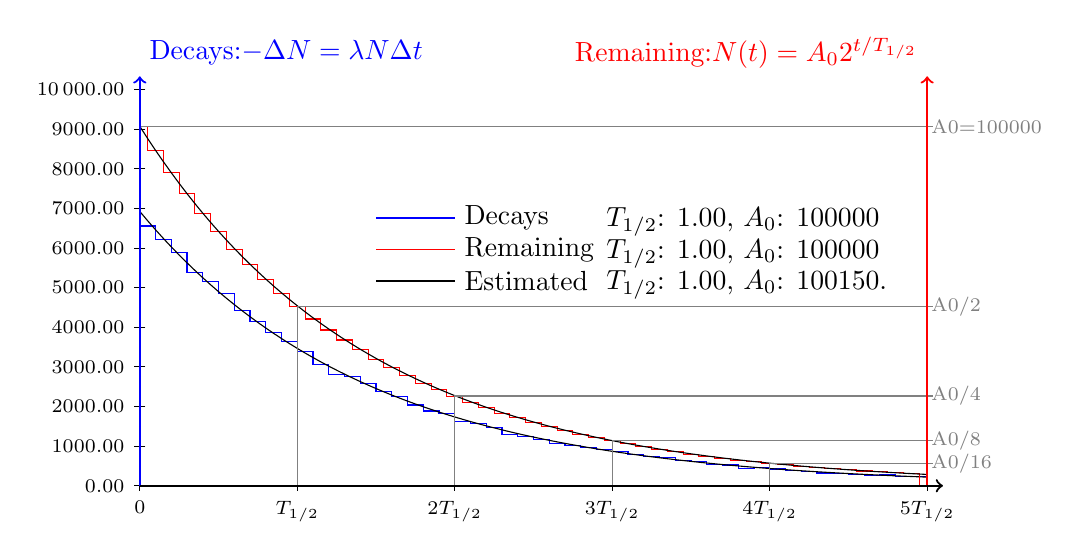
\begin{tikzpicture}[]
\begin{scope}[]
\clip (0.0,0.0) rectangle (10.0,5.0);
\begin{scope}[shift={(0.0,0.0)}]
\pgfsetxvec{\pgfpoint{2.0cm}{0cm}}
\pgfsetyvec{\pgfpoint{0cm}{0.0005cm}}
\begin{scope}[shift={(0.0,0.0)}]
\begin{scope}[draw=blue]
\pgfpathmoveto{ \pgfpointxy {5.0} {0.0}}
\pgfpathlineto{ \pgfpointxy {5.0} {230.0}}
\pgfpathlineto{ \pgfpointxy {4.9} {230.0}}
\pgfpathlineto{ \pgfpointxy {4.9} {244.0}}
\pgfpathlineto{ \pgfpointxy {4.8} {244.0}}
\pgfpathlineto{ \pgfpointxy {4.8} {271.0}}
\pgfpathlineto{ \pgfpointxy {4.7000003} {271.0}}
\pgfpathlineto{ \pgfpointxy {4.7000003} {264.0}}
\pgfpathlineto{ \pgfpointxy {4.6} {264.0}}
\pgfpathlineto{ \pgfpointxy {4.6} {290.0}}
\pgfpathlineto{ \pgfpointxy {4.5} {290.0}}
\pgfpathlineto{ \pgfpointxy {4.5} {306.0}}
\pgfpathlineto{ \pgfpointxy {4.4} {306.0}}
\pgfpathlineto{ \pgfpointxy {4.4} {322.0}}
\pgfpathlineto{ \pgfpointxy {4.3} {322.0}}
\pgfpathlineto{ \pgfpointxy {4.3} {365.0}}
\pgfpathlineto{ \pgfpointxy {4.2000003} {365.0}}
\pgfpathlineto{ \pgfpointxy {4.2000003} {394.0}}
\pgfpathlineto{ \pgfpointxy {4.1} {394.0}}
\pgfpathlineto{ \pgfpointxy {4.1} {423.0}}
\pgfpathlineto{ \pgfpointxy {4.0} {423.0}}
\pgfpathlineto{ \pgfpointxy {4.0} {457.0}}
\pgfpathlineto{ \pgfpointxy {3.9} {457.0}}
\pgfpathlineto{ \pgfpointxy {3.9} {443.0}}
\pgfpathlineto{ \pgfpointxy {3.8} {443.0}}
\pgfpathlineto{ \pgfpointxy {3.8} {525.0}}
\pgfpathlineto{ \pgfpointxy {3.7} {525.0}}
\pgfpathlineto{ \pgfpointxy {3.7} {536.0}}
\pgfpathlineto{ \pgfpointxy {3.6000001} {536.0}}
\pgfpathlineto{ \pgfpointxy {3.6000001} {613.0}}
\pgfpathlineto{ \pgfpointxy {3.5} {613.0}}
\pgfpathlineto{ \pgfpointxy {3.5} {630.0}}
\pgfpathlineto{ \pgfpointxy {3.4} {630.0}}
\pgfpathlineto{ \pgfpointxy {3.4} {714.0}}
\pgfpathlineto{ \pgfpointxy {3.3} {714.0}}
\pgfpathlineto{ \pgfpointxy {3.3} {730.0}}
\pgfpathlineto{ \pgfpointxy {3.2} {730.0}}
\pgfpathlineto{ \pgfpointxy {3.2} {785.0}}
\pgfpathlineto{ \pgfpointxy {3.1000001} {785.0}}
\pgfpathlineto{ \pgfpointxy {3.1000001} {864.0}}
\pgfpathlineto{ \pgfpointxy {3.0} {864.0}}
\pgfpathlineto{ \pgfpointxy {3.0} {910.0}}
\pgfpathlineto{ \pgfpointxy {2.9} {910.0}}
\pgfpathlineto{ \pgfpointxy {2.9} {965.0}}
\pgfpathlineto{ \pgfpointxy {2.8} {965.0}}
\pgfpathlineto{ \pgfpointxy {2.8} {1009.0}}
\pgfpathlineto{ \pgfpointxy {2.7} {1009.0}}
\pgfpathlineto{ \pgfpointxy {2.7} {1078.0}}
\pgfpathlineto{ \pgfpointxy {2.6000001} {1078.0}}
\pgfpathlineto{ \pgfpointxy {2.6000001} {1173.0}}
\pgfpathlineto{ \pgfpointxy {2.5} {1173.0}}
\pgfpathlineto{ \pgfpointxy {2.5} {1253.0}}
\pgfpathlineto{ \pgfpointxy {2.4} {1253.0}}
\pgfpathlineto{ \pgfpointxy {2.4} {1301.0}}
\pgfpathlineto{ \pgfpointxy {2.3} {1301.0}}
\pgfpathlineto{ \pgfpointxy {2.3} {1470.0}}
\pgfpathlineto{ \pgfpointxy {2.2} {1470.0}}
\pgfpathlineto{ \pgfpointxy {2.2} {1571.0}}
\pgfpathlineto{ \pgfpointxy {2.1000001} {1571.0}}
\pgfpathlineto{ \pgfpointxy {2.1000001} {1628.0}}
\pgfpathlineto{ \pgfpointxy {2.0} {1628.0}}
\pgfpathlineto{ \pgfpointxy {2.0} {1820.0}}
\pgfpathlineto{ \pgfpointxy {1.9} {1820.0}}
\pgfpathlineto{ \pgfpointxy {1.9} {1888.0}}
\pgfpathlineto{ \pgfpointxy {1.8000001} {1888.0}}
\pgfpathlineto{ \pgfpointxy {1.8000001} {2038.0}}
\pgfpathlineto{ \pgfpointxy {1.7} {2038.0}}
\pgfpathlineto{ \pgfpointxy {1.7} {2248.0}}
\pgfpathlineto{ \pgfpointxy {1.6} {2248.0}}
\pgfpathlineto{ \pgfpointxy {1.6} {2377.0}}
\pgfpathlineto{ \pgfpointxy {1.5} {2377.0}}
\pgfpathlineto{ \pgfpointxy {1.5} {2587.0}}
\pgfpathlineto{ \pgfpointxy {1.4} {2587.0}}
\pgfpathlineto{ \pgfpointxy {1.4} {2757.0}}
\pgfpathlineto{ \pgfpointxy {1.3000001} {2757.0}}
\pgfpathlineto{ \pgfpointxy {1.3000001} {2808.0}}
\pgfpathlineto{ \pgfpointxy {1.2} {2808.0}}
\pgfpathlineto{ \pgfpointxy {1.2} {3051.0}}
\pgfpathlineto{ \pgfpointxy {1.1} {3051.0}}
\pgfpathlineto{ \pgfpointxy {1.1} {3400.0}}
\pgfpathlineto{ \pgfpointxy {1.0} {3400.0}}
\pgfpathlineto{ \pgfpointxy {1.0} {3649.0}}
\pgfpathlineto{ \pgfpointxy {0.90000004} {3649.0}}
\pgfpathlineto{ \pgfpointxy {0.90000004} {3867.0}}
\pgfpathlineto{ \pgfpointxy {0.8} {3867.0}}
\pgfpathlineto{ \pgfpointxy {0.8} {4156.0}}
\pgfpathlineto{ \pgfpointxy {0.7} {4156.0}}
\pgfpathlineto{ \pgfpointxy {0.7} {4418.0}}
\pgfpathlineto{ \pgfpointxy {0.6} {4418.0}}
\pgfpathlineto{ \pgfpointxy {0.6} {4852.0}}
\pgfpathlineto{ \pgfpointxy {0.5} {4852.0}}
\pgfpathlineto{ \pgfpointxy {0.5} {5148.0}}
\pgfpathlineto{ \pgfpointxy {0.4} {5148.0}}
\pgfpathlineto{ \pgfpointxy {0.4} {5388.0}}
\pgfpathlineto{ \pgfpointxy {0.3} {5388.0}}
\pgfpathlineto{ \pgfpointxy {0.3} {5879.0}}
\pgfpathlineto{ \pgfpointxy {0.2} {5879.0}}
\pgfpathlineto{ \pgfpointxy {0.2} {6228.0}}
\pgfpathlineto{ \pgfpointxy {0.1} {6228.0}}
\pgfpathlineto{ \pgfpointxy {0.1} {6559.0}}
\pgfpathlineto{ \pgfpointxy {0.0} {6559.0}}
\pgfpathlineto{ \pgfpointxy {0.0} {0.0}}
\pgfusepath{ stroke, }
\end{scope}
\begin{scope}[black]
\pgfpathmoveto{ \pgfpointxy {0.0} {6926.170748444656}}
\pgfpathlineto{ \pgfpointxy {0.05} {6690.763194658762}}
\pgfpathlineto{ \pgfpointxy {0.1} {6463.356702121886}}
\pgfpathlineto{ \pgfpointxy {0.15} {6243.6793297680715}}
\pgfpathlineto{ \pgfpointxy {0.2} {6031.468379298172}}
\pgfpathlineto{ \pgfpointxy {0.25} {5826.470081035544}}
\pgfpathlineto{ \pgfpointxy {0.3} {5628.439290458907}}
\pgfpathlineto{ \pgfpointxy {0.35} {5437.139195049494}}
\pgfpathlineto{ \pgfpointxy {0.4} {5252.341031101914}}
\pgfpathlineto{ \pgfpointxy {0.45} {5073.823810160078}}
\pgfpathlineto{ \pgfpointxy {0.5} {4901.374054751056}}
\pgfpathlineto{ \pgfpointxy {0.55} {4734.785543100849}}
\pgfpathlineto{ \pgfpointxy {0.6} {4573.859062526792}}
\pgfpathlineto{ \pgfpointxy {0.65} {4418.402171211678}}
\pgfpathlineto{ \pgfpointxy {0.7} {4268.228968074752}}
\pgfpathlineto{ \pgfpointxy {0.75} {4123.159870464329}}
\pgfpathlineto{ \pgfpointxy {0.8} {3983.0213994062588}}
\pgfpathlineto{ \pgfpointxy {0.85} {3847.645972151357}}
\pgfpathlineto{ \pgfpointxy {0.9} {3716.87170177379}}
\pgfpathlineto{ \pgfpointxy {0.95} {3590.5422035807132}}
\pgfpathlineto{ \pgfpointxy {1.0} {3468.506408101695}}
\pgfpathlineto{ \pgfpointxy {1.05} {3350.618380434276}}
\pgfpathlineto{ \pgfpointxy {1.1} {3236.7371457296285}}
\pgfpathlineto{ \pgfpointxy {1.15} {3126.726520609644}}
\pgfpathlineto{ \pgfpointxy {1.2} {3020.4549503138232}}
\pgfpathlineto{ \pgfpointxy {1.25} {2917.7953513812467}}
\pgfpathlineto{ \pgfpointxy {1.3} {2818.624959679489}}
\pgfpathlineto{ \pgfpointxy {1.35} {2722.825183598743}}
\pgfpathlineto{ \pgfpointxy {1.4} {2630.2814622356013}}
\pgfpathlineto{ \pgfpointxy {1.45} {2540.8831283969052}}
\pgfpathlineto{ \pgfpointxy {1.5} {2454.523276259837}}
\pgfpathlineto{ \pgfpointxy {1.55} {2371.098633529997}}
\pgfpathlineto{ \pgfpointxy {1.6} {2290.509437944584}}
\pgfpathlineto{ \pgfpointxy {1.65} {2212.6593179730085}}
\pgfpathlineto{ \pgfpointxy {1.7} {2137.4551775722593}}
\pgfpathlineto{ \pgfpointxy {1.75} {2064.80708485923}}
\pgfpathlineto{ \pgfpointxy {1.8} {1994.6281645668525}}
\pgfpathlineto{ \pgfpointxy {1.85} {1926.8344941554537}}
\pgfpathlineto{ \pgfpointxy {1.9} {1861.3450034550874}}
\pgfpathlineto{ \pgfpointxy {1.95} {1798.0813777188384}}
\pgfpathlineto{ \pgfpointxy {2.0} {1736.967963971161}}
\pgfpathlineto{ \pgfpointxy {2.05} {1677.9316805392607}}
\pgfpathlineto{ \pgfpointxy {2.1} {1620.9019296593385}}
\pgfpathlineto{ \pgfpointxy {2.15} {1565.810513053182}}
\pgfpathlineto{ \pgfpointxy {2.2} {1512.5915503741492}}
\pgfpathlineto{ \pgfpointxy {2.25} {1461.181400425023}}
\pgfpathlineto{ \pgfpointxy {2.3} {1411.5185850535217}}
\pgfpathlineto{ \pgfpointxy {2.35} {1363.5437156344567}}
\pgfpathlineto{ \pgfpointxy {2.4} {1317.1994220506301}}
\pgfpathlineto{ \pgfpointxy {2.45} {1272.430284087526}}
\pgfpathlineto{ \pgfpointxy {2.5} {1229.182765159784}}
\pgfpathlineto{ \pgfpointxy {2.55} {1187.4051482901707}}
\pgfpathlineto{ \pgfpointxy {2.6} {1147.047474264514}}
\pgfpathlineto{ \pgfpointxy {2.65} {1108.0614818886354}}
\pgfpathlineto{ \pgfpointxy {2.7} {1070.4005502758316}}
\pgfpathlineto{ \pgfpointxy {2.75} {1034.0196430959022}}
\pgfpathlineto{ \pgfpointxy {2.8} {998.8752547190447}}
\pgfpathlineto{ \pgfpointxy {2.85} {964.9253581902192}}
\pgfpathlineto{ \pgfpointxy {2.9} {932.1293549717678}}
\pgfpathlineto{ \pgfpointxy {2.95} {900.4480263941834}}
\pgfpathlineto{ \pgfpointxy {3.0} {869.8434867569833}}
\pgfpathlineto{ \pgfpointxy {3.05} {840.2791380235891}}
\pgfpathlineto{ \pgfpointxy {3.1} {811.7196260560456}}
\pgfpathlineto{ \pgfpointxy {3.15} {784.1307983372425}}
\pgfpathlineto{ \pgfpointxy {3.2} {757.4796631300716}}
\pgfpathlineto{ \pgfpointxy {3.25} {731.7343500246944}}
\pgfpathlineto{ \pgfpointxy {3.3} {706.8640718267297}}
\pgfpathlineto{ \pgfpointxy {3.35} {682.8390877407925}}
\pgfpathlineto{ \pgfpointxy {3.4} {659.6306678053544}}
\pgfpathlineto{ \pgfpointxy {3.45} {637.2110585363964}}
\pgfpathlineto{ \pgfpointxy {3.5} {615.5534497387707}}
\pgfpathlineto{ \pgfpointxy {3.55} {594.6319424455797}}
\pgfpathlineto{ \pgfpointxy {3.6} {574.4215179472371}}
\pgfpathlineto{ \pgfpointxy {3.65} {554.8980078731744}}
\pgfpathlineto{ \pgfpointxy {3.7} {536.0380652904098}}
\pgfpathlineto{ \pgfpointxy {3.75} {517.8191367844275}}
\pgfpathlineto{ \pgfpointxy {3.8} {500.21943548897235}}
\pgfpathlineto{ \pgfpointxy {3.85} {483.21791503251205}}
\pgfpathlineto{ \pgfpointxy {3.9} {466.7942443702102}}
\pgfpathlineto{ \pgfpointxy {3.95} {450.9287834713141}}
\pgfpathlineto{ \pgfpointxy {4.0} {435.60255983288187}}
\pgfpathlineto{ \pgfpointxy {4.05} {420.7972457917633}}
\pgfpathlineto{ \pgfpointxy {4.1} {406.49513660770606}}
\pgfpathlineto{ \pgfpointxy {4.15} {392.6791292913727}}
\pgfpathlineto{ \pgfpointxy {4.2} {379.33270215195887}}
\pgfpathlineto{ \pgfpointxy {4.25} {366.4398950399428}}
\pgfpathlineto{ \pgfpointxy {4.3} {353.98529026135225}}
\pgfpathlineto{ \pgfpointxy {4.35} {341.9539941407178}}
\pgfpathlineto{ \pgfpointxy {4.4} {330.3316192106658}}
\pgfpathlineto{ \pgfpointxy {4.45} {319.1042670068554}}
\pgfpathlineto{ \pgfpointxy {4.5} {308.2585114476826}}
\pgfpathlineto{ \pgfpointxy {4.55} {297.78138277887587}}
\pgfpathlineto{ \pgfpointxy {4.6} {287.6603520637874}}
\pgfpathlineto{ \pgfpointxy {4.65} {277.8833162008277}}
\pgfpathlineto{ \pgfpointxy {4.7} {268.43858345013155}}
\pgfpathlineto{ \pgfpointxy {4.75} {259.31485945214376}}
\pgfpathlineto{ \pgfpointxy {4.8} {250.50123372140794}}
\pgfpathlineto{ \pgfpointxy {4.85} {241.9871665994058}}
\pgfpathlineto{ \pgfpointxy {4.9} {233.76247665084537}}
\pgfpathlineto{ \pgfpointxy {4.95} {225.81732848832505}}
\pgfpathlineto{ \pgfpointxy {5.0} {218.14222101081447}}
\pgfusepath{ stroke, }
\end{scope}
\end{scope}
\pgfsetxvec{\pgfpoint{1cm}{0cm}}
\pgfsetyvec{\pgfpoint{0cm}{1cm}}
\end{scope}
\end{scope}
\begin{scope}[shift={(0.0,0.0)}]
\pgfsetxvec{\pgfpoint{2.0cm}{0cm}}
\pgfsetyvec{\pgfpoint{0cm}{0.0005cm}}
\begin{scope}[shift={(0.0,0.0)}]
\begin{scope}[yshift=0cm]
\draw[black] [shift={(0.0,0.0)}] (0,2pt) -- (0,-2pt) node[below]{ \scriptsize{$0$}};
\draw[black] [shift={(1.0,0.0)}] (0,2pt) -- (0,-2pt) node[below]{ \scriptsize{$T_{1/2}$}};
\draw[black] [shift={(2.0,0.0)}] (0,2pt) -- (0,-2pt) node[below]{ \scriptsize{$2T_{1/2}$}};
\draw[black] [shift={(3.0,0.0)}] (0,2pt) -- (0,-2pt) node[below]{ \scriptsize{$3T_{1/2}$}};
\draw[black] [shift={(4.0,0.0)}] (0,2pt) -- (0,-2pt) node[below]{ \scriptsize{$4T_{1/2}$}};
\draw[black] [shift={(5.0,0.0)}] (0,2pt) -- (0,-2pt) node[below]{ \scriptsize{$5T_{1/2}$}};
\end{scope}
\begin{scope}[xshift=0cm]
\draw[black] [shift={(0.0,0.0)}] (2pt,0) -- (-2pt,0) node[left]{ \scriptsize{\num[round-mode=places,round-precision=2]{0}}};
\draw[black] [shift={(0.0,1000.0)}] (2pt,0) -- (-2pt,0) node[left]{ \scriptsize{\num[round-mode=places,round-precision=2]{1000}}};
\draw[black] [shift={(0.0,2000.0)}] (2pt,0) -- (-2pt,0) node[left]{ \scriptsize{\num[round-mode=places,round-precision=2]{2000}}};
\draw[black] [shift={(0.0,3000.0)}] (2pt,0) -- (-2pt,0) node[left]{ \scriptsize{\num[round-mode=places,round-precision=2]{3000}}};
\draw[black] [shift={(0.0,4000.0)}] (2pt,0) -- (-2pt,0) node[left]{ \scriptsize{\num[round-mode=places,round-precision=2]{4000}}};
\draw[black] [shift={(0.0,5000.0)}] (2pt,0) -- (-2pt,0) node[left]{ \scriptsize{\num[round-mode=places,round-precision=2]{5000}}};
\draw[black] [shift={(0.0,6000.0)}] (2pt,0) -- (-2pt,0) node[left]{ \scriptsize{\num[round-mode=places,round-precision=2]{6000}}};
\draw[black] [shift={(0.0,7000.0)}] (2pt,0) -- (-2pt,0) node[left]{ \scriptsize{\num[round-mode=places,round-precision=2]{7000}}};
\draw[black] [shift={(0.0,8000.0)}] (2pt,0) -- (-2pt,0) node[left]{ \scriptsize{\num[round-mode=places,round-precision=2]{8000}}};
\draw[black] [shift={(0.0,9000.0)}] (2pt,0) -- (-2pt,0) node[left]{ \scriptsize{\num[round-mode=places,round-precision=2]{9000}}};
\draw[black] [shift={(0.0,10000.0)}] (2pt,0) -- (-2pt,0) node[left]{ \scriptsize{\num[round-mode=places,round-precision=2]{10000}}};
\end{scope}
\end{scope}
\pgfsetxvec{\pgfpoint{1cm}{0cm}}
\pgfsetyvec{\pgfpoint{0cm}{1cm}}
\end{scope}
\begin{scope}[]
\clip (0.0,0.0) rectangle (10.0,5.0);
\begin{scope}[shift={(0.0,0.0)}]
\pgfsetxvec{\pgfpoint{2.0cm}{0cm}}
\pgfsetyvec{\pgfpoint{0cm}{0.00005cm}}
\begin{scope}[shift={(0.0,0.0)}]
\begin{scope}[draw=red]
\pgfpathmoveto{ \pgfpointxy {4.95} {0.0}}
\pgfpathlineto{ \pgfpointxy {4.95} {3348.0}}
\pgfpathlineto{ \pgfpointxy {4.85} {3348.0}}
\pgfpathlineto{ \pgfpointxy {4.85} {3592.0}}
\pgfpathlineto{ \pgfpointxy {4.75} {3592.0}}
\pgfpathlineto{ \pgfpointxy {4.75} {3863.0}}
\pgfpathlineto{ \pgfpointxy {4.65} {3863.0}}
\pgfpathlineto{ \pgfpointxy {4.65} {4127.0}}
\pgfpathlineto{ \pgfpointxy {4.5499997} {4127.0}}
\pgfpathlineto{ \pgfpointxy {4.5499997} {4417.0}}
\pgfpathlineto{ \pgfpointxy {4.45} {4417.0}}
\pgfpathlineto{ \pgfpointxy {4.45} {4723.0}}
\pgfpathlineto{ \pgfpointxy {4.35} {4723.0}}
\pgfpathlineto{ \pgfpointxy {4.35} {5045.0}}
\pgfpathlineto{ \pgfpointxy {4.25} {5045.0}}
\pgfpathlineto{ \pgfpointxy {4.25} {5410.0}}
\pgfpathlineto{ \pgfpointxy {4.15} {5410.0}}
\pgfpathlineto{ \pgfpointxy {4.15} {5804.0}}
\pgfpathlineto{ \pgfpointxy {4.0499997} {5804.0}}
\pgfpathlineto{ \pgfpointxy {4.0499997} {6227.0}}
\pgfpathlineto{ \pgfpointxy {3.95} {6227.0}}
\pgfpathlineto{ \pgfpointxy {3.95} {6684.0}}
\pgfpathlineto{ \pgfpointxy {3.8500001} {6684.0}}
\pgfpathlineto{ \pgfpointxy {3.8500001} {7127.0}}
\pgfpathlineto{ \pgfpointxy {3.75} {7127.0}}
\pgfpathlineto{ \pgfpointxy {3.75} {7652.0}}
\pgfpathlineto{ \pgfpointxy {3.65} {7652.0}}
\pgfpathlineto{ \pgfpointxy {3.65} {8188.0}}
\pgfpathlineto{ \pgfpointxy {3.5500002} {8188.0}}
\pgfpathlineto{ \pgfpointxy {3.5500002} {8801.0}}
\pgfpathlineto{ \pgfpointxy {3.45} {8801.0}}
\pgfpathlineto{ \pgfpointxy {3.45} {9431.0}}
\pgfpathlineto{ \pgfpointxy {3.3500001} {9431.0}}
\pgfpathlineto{ \pgfpointxy {3.3500001} {10145.0}}
\pgfpathlineto{ \pgfpointxy {3.25} {10145.0}}
\pgfpathlineto{ \pgfpointxy {3.25} {10875.0}}
\pgfpathlineto{ \pgfpointxy {3.15} {10875.0}}
\pgfpathlineto{ \pgfpointxy {3.15} {11660.0}}
\pgfpathlineto{ \pgfpointxy {3.0500002} {11660.0}}
\pgfpathlineto{ \pgfpointxy {3.0500002} {12524.0}}
\pgfpathlineto{ \pgfpointxy {2.95} {12524.0}}
\pgfpathlineto{ \pgfpointxy {2.95} {13434.0}}
\pgfpathlineto{ \pgfpointxy {2.8500001} {13434.0}}
\pgfpathlineto{ \pgfpointxy {2.8500001} {14399.0}}
\pgfpathlineto{ \pgfpointxy {2.75} {14399.0}}
\pgfpathlineto{ \pgfpointxy {2.75} {15408.0}}
\pgfpathlineto{ \pgfpointxy {2.65} {15408.0}}
\pgfpathlineto{ \pgfpointxy {2.65} {16486.0}}
\pgfpathlineto{ \pgfpointxy {2.5500002} {16486.0}}
\pgfpathlineto{ \pgfpointxy {2.5500002} {17659.0}}
\pgfpathlineto{ \pgfpointxy {2.45} {17659.0}}
\pgfpathlineto{ \pgfpointxy {2.45} {18912.0}}
\pgfpathlineto{ \pgfpointxy {2.3500001} {18912.0}}
\pgfpathlineto{ \pgfpointxy {2.3500001} {20213.0}}
\pgfpathlineto{ \pgfpointxy {2.25} {20213.0}}
\pgfpathlineto{ \pgfpointxy {2.25} {21683.0}}
\pgfpathlineto{ \pgfpointxy {2.15} {21683.0}}
\pgfpathlineto{ \pgfpointxy {2.15} {23254.0}}
\pgfpathlineto{ \pgfpointxy {2.0500002} {23254.0}}
\pgfpathlineto{ \pgfpointxy {2.0500002} {24882.0}}
\pgfpathlineto{ \pgfpointxy {1.95} {24882.0}}
\pgfpathlineto{ \pgfpointxy {1.95} {26702.0}}
\pgfpathlineto{ \pgfpointxy {1.85} {26702.0}}
\pgfpathlineto{ \pgfpointxy {1.85} {28590.0}}
\pgfpathlineto{ \pgfpointxy {1.7500001} {28590.0}}
\pgfpathlineto{ \pgfpointxy {1.7500001} {30628.0}}
\pgfpathlineto{ \pgfpointxy {1.6500001} {30628.0}}
\pgfpathlineto{ \pgfpointxy {1.6500001} {32876.0}}
\pgfpathlineto{ \pgfpointxy {1.5500001} {32876.0}}
\pgfpathlineto{ \pgfpointxy {1.5500001} {35253.0}}
\pgfpathlineto{ \pgfpointxy {1.45} {35253.0}}
\pgfpathlineto{ \pgfpointxy {1.45} {37840.0}}
\pgfpathlineto{ \pgfpointxy {1.35} {37840.0}}
\pgfpathlineto{ \pgfpointxy {1.35} {40597.0}}
\pgfpathlineto{ \pgfpointxy {1.2500001} {40597.0}}
\pgfpathlineto{ \pgfpointxy {1.2500001} {43405.0}}
\pgfpathlineto{ \pgfpointxy {1.1500001} {43405.0}}
\pgfpathlineto{ \pgfpointxy {1.1500001} {46456.0}}
\pgfpathlineto{ \pgfpointxy {1.0500001} {46456.0}}
\pgfpathlineto{ \pgfpointxy {1.0500001} {49856.0}}
\pgfpathlineto{ \pgfpointxy {0.95} {49856.0}}
\pgfpathlineto{ \pgfpointxy {0.95} {53505.0}}
\pgfpathlineto{ \pgfpointxy {0.85} {53505.0}}
\pgfpathlineto{ \pgfpointxy {0.85} {57372.0}}
\pgfpathlineto{ \pgfpointxy {0.75} {57372.0}}
\pgfpathlineto{ \pgfpointxy {0.75} {61528.0}}
\pgfpathlineto{ \pgfpointxy {0.65} {61528.0}}
\pgfpathlineto{ \pgfpointxy {0.65} {65946.0}}
\pgfpathlineto{ \pgfpointxy {0.55} {65946.0}}
\pgfpathlineto{ \pgfpointxy {0.55} {70798.0}}
\pgfpathlineto{ \pgfpointxy {0.45} {70798.0}}
\pgfpathlineto{ \pgfpointxy {0.45} {75946.0}}
\pgfpathlineto{ \pgfpointxy {0.35} {75946.0}}
\pgfpathlineto{ \pgfpointxy {0.35} {81334.0}}
\pgfpathlineto{ \pgfpointxy {0.25} {81334.0}}
\pgfpathlineto{ \pgfpointxy {0.25} {87213.0}}
\pgfpathlineto{ \pgfpointxy {0.15} {87213.0}}
\pgfpathlineto{ \pgfpointxy {0.15} {93441.0}}
\pgfpathlineto{ \pgfpointxy {0.05} {93441.0}}
\pgfpathlineto{ \pgfpointxy {0.05} {100000.0}}
\pgfpathlineto{ \pgfpointxy {-0.05} {100000.0}}
\pgfpathlineto{ \pgfpointxy {-0.05} {0.0}}
\pgfusepath{ stroke, }
\end{scope}
\begin{scope}[black]
\pgfpathmoveto{ \pgfpointxy {0.0} {100149.51712276821}}
\pgfpathlineto{ \pgfpointxy {0.05} {96745.62286503517}}
\pgfpathlineto{ \pgfpointxy {0.1} {93457.42058915786}}
\pgfpathlineto{ \pgfpointxy {0.15} {90280.978141652}}
\pgfpathlineto{ \pgfpointxy {0.2} {87212.4970155555}}
\pgfpathlineto{ \pgfpointxy {0.25} {84248.3078080339}}
\pgfpathlineto{ \pgfpointxy {0.3} {81384.86583237312}}
\pgfpathlineto{ \pgfpointxy {0.35} {78618.74687911248}}
\pgfpathlineto{ \pgfpointxy {0.4} {75946.64312124884}}
\pgfpathlineto{ \pgfpointxy {0.45} {73365.35915861506}}
\pgfpathlineto{ \pgfpointxy {0.5} {70871.80819670274}}
\pgfpathlineto{ \pgfpointxy {0.55} {68463.00835535962}}
\pgfpathlineto{ \pgfpointxy {0.6} {66136.0791029473}}
\pgfpathlineto{ \pgfpointxy {0.65} {63888.23781169537}}
\pgfpathlineto{ \pgfpointxy {0.7} {61716.796430132556}}
\pgfpathlineto{ \pgfpointxy {0.75} {59619.15826861566}}
\pgfpathlineto{ \pgfpointxy {0.8} {57592.814894112445}}
\pgfpathlineto{ \pgfpointxy {0.85} {55635.34313052484}}
\pgfpathlineto{ \pgfpointxy {0.9} {53744.40216096576}}
\pgfpathlineto{ \pgfpointxy {0.95} {51917.730728523915}}
\pgfpathlineto{ \pgfpointxy {1.0} {50153.14443216944}}
\pgfpathlineto{ \pgfpointxy {1.05} {48448.53311456674}}
\pgfpathlineto{ \pgfpointxy {1.1} {46801.858338670376}}
\pgfpathlineto{ \pgfpointxy {1.15} {45211.15095008709}}
\pgfpathlineto{ \pgfpointxy {1.2} {43674.50872228831}}
\pgfpathlineto{ \pgfpointxy {1.25} {42190.09408185753}}
\pgfpathlineto{ \pgfpointxy {1.3} {40756.13191105239}}
\pgfpathlineto{ \pgfpointxy {1.35} {39370.90742505332}}
\pgfpathlineto{ \pgfpointxy {1.4} {38032.764121360735}}
\pgfpathlineto{ \pgfpointxy {1.45} {36740.10179888826}}
\pgfpathlineto{ \pgfpointxy {1.5} {35491.37464438326}}
\pgfpathlineto{ \pgfpointxy {1.55} {34285.08938388645}}
\pgfpathlineto{ \pgfpointxy {1.6} {33119.80349701976}}
\pgfpathlineto{ \pgfpointxy {1.65} {31994.123491967377}}
\pgfpathlineto{ \pgfpointxy {1.7} {30906.703239086783}}
\pgfpathlineto{ \pgfpointxy {1.75} {29856.242361157398}}
\pgfpathlineto{ \pgfpointxy {1.8} {28841.484678341516}}
\pgfpathlineto{ \pgfpointxy {1.85} {27861.216705998162}}
\pgfpathlineto{ \pgfpointxy {1.9} {26914.266203553427}}
\pgfpathlineto{ \pgfpointxy {1.95} {25999.500772691987}}
\pgfpathlineto{ \pgfpointxy {2.0} {25115.826503193468}}
\pgfpathlineto{ \pgfpointxy {2.05} {24262.186664794248}}
\pgfpathlineto{ \pgfpointxy {2.1} {23437.560443510498}}
\pgfpathlineto{ \pgfpointxy {2.15} {22640.961720911168}}
\pgfpathlineto{ \pgfpointxy {2.2} {21871.437894881234}}
\pgfpathlineto{ \pgfpointxy {2.25} {21128.068740464954}}
\pgfpathlineto{ \pgfpointxy {2.3} {20409.965309426967}}
\pgfpathlineto{ \pgfpointxy {2.35} {19716.268867215207}}
\pgfpathlineto{ \pgfpointxy {2.4} {19046.14986605453}}
\pgfpathlineto{ \pgfpointxy {2.45} {18398.806952942792}}
\pgfpathlineto{ \pgfpointxy {2.5} {17773.466011363525}}
\pgfpathlineto{ \pgfpointxy {2.55} {17169.379235568784}}
\pgfpathlineto{ \pgfpointxy {2.6} {16585.824236325483}}
\pgfpathlineto{ \pgfpointxy {2.65} {16022.103177055762}}
\pgfpathlineto{ \pgfpointxy {2.7} {15477.541939338244}}
\pgfpathlineto{ \pgfpointxy {2.75} {14951.489316772395}}
\pgfpathlineto{ \pgfpointxy {2.8} {14443.316236241903}}
\pgfpathlineto{ \pgfpointxy {2.85} {13952.415005645857}}
\pgfpathlineto{ \pgfpointxy {2.9} {13478.198587198156}}
\pgfpathlineto{ \pgfpointxy {2.95} {13020.099895426034}}
\pgfpathlineto{ \pgfpointxy {3.0} {12577.571119028411}}
\pgfpathlineto{ \pgfpointxy {3.05} {12150.08306578291}}
\pgfpathlineto{ \pgfpointxy {3.1} {11737.124529718276}}
\pgfpathlineto{ \pgfpointxy {3.15} {11338.20167979549}}
\pgfpathlineto{ \pgfpointxy {3.2} {10952.83746936635}}
\pgfpathlineto{ \pgfpointxy {3.25} {10580.571065703547}}
\pgfpathlineto{ \pgfpointxy {3.3} {10220.957298919873}}
\pgfpathlineto{ \pgfpointxy {3.35} {9873.566129617686}}
\pgfpathlineto{ \pgfpointxy {3.4} {9537.982134631926}}
\pgfpathlineto{ \pgfpointxy {3.45} {9213.804010251803}}
\pgfpathlineto{ \pgfpointxy {3.5} {8900.644092327007}}
\pgfpathlineto{ \pgfpointxy {3.55} {8598.12789268465}}
\pgfpathlineto{ \pgfpointxy {3.6} {8305.89365130247}}
\pgfpathlineto{ \pgfpointxy {3.65} {8023.591903702907}}
\pgfpathlineto{ \pgfpointxy {3.7} {7750.885063050566}}
\pgfpathlineto{ \pgfpointxy {3.75} {7487.447016453448}}
\pgfpathlineto{ \pgfpointxy {3.8} {7232.9627349851335}}
\pgfpathlineto{ \pgfpointxy {3.85} {6987.12789696158}}
\pgfpathlineto{ \pgfpointxy {3.9} {6749.648524022027}}
\pgfpathlineto{ \pgfpointxy {3.95} {6520.240629578851}}
\pgfpathlineto{ \pgfpointxy {4.0} {6298.62987921593}}
\pgfpathlineto{ \pgfpointxy {4.05} {6084.551262629423}}
\pgfpathlineto{ \pgfpointxy {4.1} {5877.748776718706}}
\pgfpathlineto{ \pgfpointxy {4.15} {5677.975119448398}}
\pgfpathlineto{ \pgfpointxy {4.2} {5484.991394115514}}
\pgfpathlineto{ \pgfpointxy {4.25} {5298.566823667932}}
\pgfpathlineto{ \pgfpointxy {4.3} {5118.4784747327185}}
\pgfpathlineto{ \pgfpointxy {4.35} {4944.510991024184}}
\pgfpathlineto{ \pgfpointxy {4.4} {4776.456335812881}}
\pgfpathlineto{ \pgfpointxy {4.45} {4614.113543147633}}
\pgfpathlineto{ \pgfpointxy {4.5} {4457.288477533037}}
\pgfpathlineto{ \pgfpointxy {4.55} {4305.793601775066}}
\pgfpathlineto{ \pgfpointxy {4.6} {4159.447752717211}}
\pgfpathlineto{ \pgfpointxy {4.65} {4018.0759245988706}}
\pgfpathlineto{ \pgfpointxy {4.7} {3881.509059777031}}
\pgfpathlineto{ \pgfpointxy {4.75} {3749.5838465609004}}
\pgfpathlineto{ \pgfpointxy {4.8} {3622.142523917763}}
\pgfpathlineto{ \pgfpointxy {4.85} {3499.032692816526}}
\pgfpathlineto{ \pgfpointxy {4.9} {3380.1071339833443}}
\pgfpathlineto{ \pgfpointxy {4.95} {3265.2236318513847}}
\pgfpathlineto{ \pgfpointxy {5.0} {3154.2448044941984}}
\pgfusepath{ stroke, }
\end{scope}
\end{scope}
\pgfsetxvec{\pgfpoint{1cm}{0cm}}
\pgfsetyvec{\pgfpoint{0cm}{1cm}}
\end{scope}
\end{scope}
\begin{scope}[shift={(0.0,0.0)}]
\pgfsetxvec{\pgfpoint{2.0cm}{0cm}}
\pgfsetyvec{\pgfpoint{0cm}{0.00005cm}}
\begin{scope}[shift={(0.0,0.0)}]
\begin{scope}[gray]
\pgfpathmoveto{ \pgfpointxy {0.0} {0.0}}
\pgfpathlineto{ \pgfpointxy {0.0} {100000.0}}
\pgfpathlineto{ \pgfpointxy {5.0} {100000.0}}
\pgfusepath{ stroke, }
\end{scope}
\begin{scope}[gray]
\pgfpathmoveto{ \pgfpointxy {1.0} {0.0}}
\pgfpathlineto{ \pgfpointxy {1.0} {50000.0}}
\pgfpathlineto{ \pgfpointxy {5.0} {50000.0}}
\pgfusepath{ stroke, }
\end{scope}
\begin{scope}[gray]
\pgfpathmoveto{ \pgfpointxy {2.0} {0.0}}
\pgfpathlineto{ \pgfpointxy {2.0} {25000.0}}
\pgfpathlineto{ \pgfpointxy {5.0} {25000.0}}
\pgfusepath{ stroke, }
\end{scope}
\begin{scope}[gray]
\pgfpathmoveto{ \pgfpointxy {3.0} {0.0}}
\pgfpathlineto{ \pgfpointxy {3.0} {12500.0}}
\pgfpathlineto{ \pgfpointxy {5.0} {12500.0}}
\pgfusepath{ stroke, }
\end{scope}
\begin{scope}[gray]
\pgfpathmoveto{ \pgfpointxy {4.0} {0.0}}
\pgfpathlineto{ \pgfpointxy {4.0} {6250.0}}
\pgfpathlineto{ \pgfpointxy {5.0} {6250.0}}
\pgfusepath{ stroke, }
\end{scope}
\begin{scope}[xshift=10cm]
\draw[gray] [shift={(0.0,100000.0)}] (2pt,0) -- (-2pt,0) node[right]{ \scriptsize{A0=100000}};
\draw[gray] [shift={(0.0,50000.0)}] (2pt,0) -- (-2pt,0) node[right]{ \scriptsize{A0/2}};
\draw[gray] [shift={(0.0,25000.0)}] (2pt,0) -- (-2pt,0) node[right]{ \scriptsize{A0/4}};
\draw[gray] [shift={(0.0,12500.0)}] (2pt,0) -- (-2pt,0) node[right]{ \scriptsize{A0/8}};
\draw[gray] [shift={(0.0,6250.0)}] (2pt,0) -- (-2pt,0) node[right]{ \scriptsize{A0/16}};
\end{scope}
\end{scope}
\pgfsetxvec{\pgfpoint{1cm}{0cm}}
\pgfsetyvec{\pgfpoint{0cm}{1cm}}
\end{scope}
\node[right,blue] at (0.0,5.5) {Decays:$-\Delta N = \lambda N \Delta t$};
\node[left,red] at (10.0,5.5) {Remaining:$N(t) = A_0 2^{t/T_{1/2}}$};
\draw[blue,thick,->] (0.0,0.0) -- (0.0,5.2);
\draw[red,thick,->] (10.0,0.0) -- (10.0,5.2);
\draw[black,thick,->] (0.0,0.0) -- (10.2,0.0);
\draw[blue] (3.0,3.4) -- (4.0,3.4);
\node[right,] at (4.0,3.4) {Decays};
\node[right] at (5.8,3.35) {$T_{1/2}$: 1.00, $A_0$: 100000};
\draw[red] (3.0,3.0) -- (4.0,3.0);
\node[right,] at (4.0,3.0) {Remaining};
\node[right] at (5.8,2.95) {$T_{1/2}$: 1.00, $A_0$: 100000};
\draw[black] (3.0,2.6) -- (4.0,2.6);
\node[right,] at (4.0,2.6) {Estimated};
\node[right] at (5.8,2.55) {$T_{1/2}$:  1.00, $A_0$: 100150.};
\end{tikzpicture}
%%% Local Variables: 
%%% mode: latex 
%%% TeX-master: "master" 
%%% End:


  \caption{Graph of radioactive decay.}
\end{figure}

\begin{figure}[H]
  \centering
  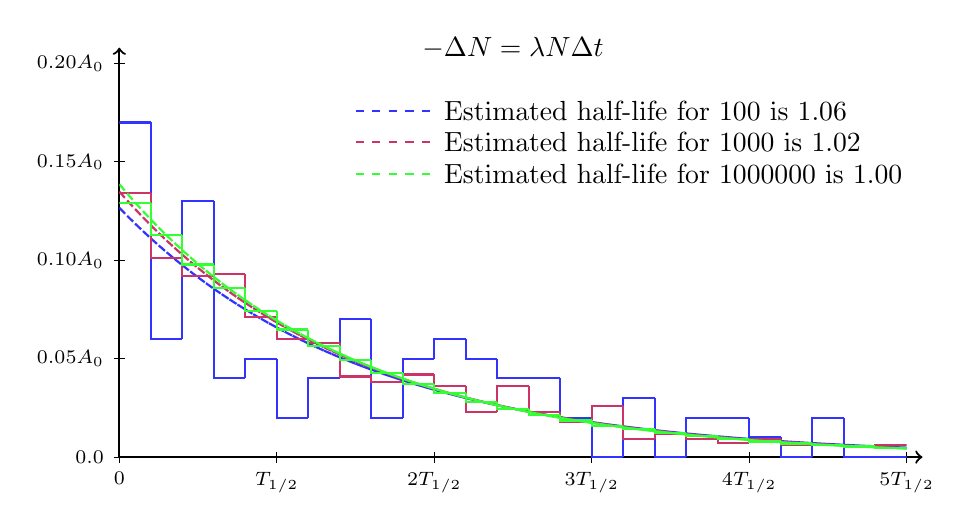
\begin{tikzpicture}
\node[] at (5.0,5.2) {$-\Delta N = \lambda N \Delta t$};
\draw[thick,->] (0.0,0.0) -- (0.0,5.2);
\draw[thick,->] (0.0,0.0) -- (10.2,0.0);
\draw (0,0cm + 2pt) -- (0, 0cm-2pt) node[below] {\scriptsize $0$};
\draw (2,0cm + 2pt) -- (2, 0cm-2pt) node[below] {\scriptsize $T_{1/2}$};
\draw (4,0cm + 2pt) -- (4, 0cm-2pt) node[below] {\scriptsize $2T_{1/2}$};
\draw (6,0cm + 2pt) -- (6, 0cm-2pt) node[below] {\scriptsize $3T_{1/2}$};
\draw (8,0cm + 2pt) -- (8, 0cm-2pt) node[below] {\scriptsize $4T_{1/2}$};
\draw (10,0cm + 2pt) -- (10, 0cm-2pt) node[below] {\scriptsize $5T_{1/2}$};
\draw (0cm+2pt,0.    ) -- (0cm-2pt,0.    ) node[left] {\scriptsize $0.0$};
\draw (0cm+2pt,1.25    ) -- (0cm-2pt,1.25    ) node[left] {\scriptsize $0.05 A_0$};
\draw (0cm+2pt,2.5    ) -- (0cm-2pt,2.5    ) node[left] {\scriptsize $0.10 A_0$};
\draw (0cm+2pt,3.750000093132256    ) -- (0cm-2pt,3.750000093132256    ) node[left] {\scriptsize $0.15 A_0$};
\draw (0cm+2pt,5.    ) -- (0cm-2pt,5.    ) node[left] {\scriptsize $0.20 A_0$};
\begin{scope}[]
\clip (0,0) rectangle (10,5);
\draw[dashed,blue!80,thick] (3.0,4.4) -- (4.0,4.4);
\node[right,] at (4.0,4.4) {Estimated half-life for 100 is  1.06};
\begin{scope}[blue!80,thick]
\draw[] (0.0,4.249999936670066) -- (0.4,4.249999936670066);
\draw (0.4,4.249999936670066) -- (0.4,1.4999999776482584) -- (0.8,1.4999999776482584);
\draw (0.8,1.4999999776482584) -- (0.8,3.249999951571227) -- (1.2,3.249999951571227);
\draw (1.2,3.249999951571227) -- (1.2,0.999999985098839) -- (1.6,0.999999985098839);
\draw (1.6,0.999999985098839) -- (1.6,1.2499999813735487) -- (2.0,1.2499999813735487);
\draw (2.0,1.2499999813735487) -- (2.0,0.4999999925494195) -- (2.4,0.4999999925494195);
\draw (2.4,0.4999999925494195) -- (2.4,0.999999985098839) -- (2.8,0.999999985098839);
\draw (2.8,0.999999985098839) -- (2.8,1.7499999739229684) -- (3.2,1.7499999739229684);
\draw (3.2,1.7499999739229684) -- (3.2,0.4999999925494195) -- (3.6000001,0.4999999925494195);
\draw (3.6000001,0.4999999925494195) -- (3.6000001,1.2499999813735487) -- (4.0,1.2499999813735487);
\draw (4.0,1.2499999813735487) -- (4.0,1.4999999776482584) -- (4.4,1.4999999776482584);
\draw (4.4,1.4999999776482584) -- (4.4,1.2499999813735487) -- (4.8,1.2499999813735487);
\draw (4.8,1.2499999813735487) -- (4.8,0.999999985098839) -- (5.2000003,0.999999985098839);
\draw (5.2000003,0.999999985098839) -- (5.2000003,0.999999985098839) -- (5.6,0.999999985098839);
\draw (5.6,0.999999985098839) -- (5.6,0.4999999925494195) -- (6.0,0.4999999925494195);
\draw (6.0,0.4999999925494195) -- (6.0,0.0) -- (6.4,0.0);
\draw (6.4,0.0) -- (6.4,0.7499999888241292) -- (6.8,0.7499999888241292);
\draw (6.8,0.7499999888241292) -- (6.8,0.0) -- (7.2000003,0.0);
\draw (7.2000003,0.0) -- (7.2000003,0.4999999925494195) -- (7.6,0.4999999925494195);
\draw (7.6,0.4999999925494195) -- (7.6,0.4999999925494195) -- (8.0,0.4999999925494195);
\draw (8.0,0.4999999925494195) -- (8.0,0.24999999627470976) -- (8.400001,0.24999999627470976);
\draw (8.400001,0.24999999627470976) -- (8.400001,0.0) -- (8.8,0.0);
\draw (8.8,0.0) -- (8.8,0.4999999925494195) -- (9.2,0.4999999925494195);
\draw (9.2,0.4999999925494195) -- (9.2,0.0) -- (9.6,0.0);
\draw (9.6,0.0) -- (9.6,0.0) -- (10.0,0.0);
\end{scope}
\begin{scope}[dashed,blue!80,thick]
\draw[] (0.0,3.1663723527596903) -- (0.1,3.0644451708500897);
\draw[] (0.1,3.0644451708500897) -- (0.2,2.9657990782296175);
\draw[] (0.2,2.9657990782296175) -- (0.3,2.870328454918191);
\draw[] (0.3,2.870328454918191) -- (0.4,2.77793108089812);
\draw[] (0.4,2.77793108089812) -- (0.5,2.6885080266675407);
\draw[] (0.5,2.6885080266675407) -- (0.6,2.6019635473169904);
\draw[] (0.6,2.6019635473169904) -- (0.7,2.518204980015712);
\draw[] (0.7,2.518204980015712) -- (0.8,2.4371426447979294);
\draw[] (0.8,2.4371426447979294) -- (0.9,2.358689748542864);
\draw[] (0.9,2.358689748542864) -- (1.0,2.282762292045683);
\draw[] (1.0,2.282762292045683) -- (1.1,2.209278980079885);
\draw[] (1.1,2.209278980079885) -- (1.2,2.138161134354825);
\draw[] (1.2,2.138161134354825) -- (1.3,2.0693326092751776);
\draw[] (1.3,2.0693326092751776) -- (1.4,2.0027197104121526);
\draw[] (1.4,2.0027197104121526) -- (1.5,1.938251115599161);
\draw[] (1.5,1.938251115599161) -- (1.6,1.8758577985674558);
\draw[] (1.6,1.8758577985674558) -- (1.7,1.8154729550399773);
\draw[] (1.7,1.8154729550399773) -- (1.8,1.7570319312042806);
\draw[] (1.8,1.7570319312042806) -- (1.9,1.7004721544879549);
\draw[] (1.9,1.7004721544879549) -- (2.0,1.6457330665624168);
\draw[] (2.0,1.6457330665624168) -- (2.1,1.5927560585033511);
\draw[] (2.1,1.5927560585033511) -- (2.2,1.5414844080383652);
\draw[] (2.2,1.5414844080383652) -- (2.3,1.4918632188146783);
\draw[] (2.3,1.4918632188146783) -- (2.4,1.4438393616218137);
\draw[] (2.4,1.4438393616218137) -- (2.5,1.3973614175063644);
\draw[] (2.5,1.3973614175063644) -- (2.6,1.3523796227179237);
\draw[] (2.6,1.3523796227179237) -- (2.7,1.3088458154272342);
\draw[] (2.7,1.3088458154272342) -- (2.8,1.2667133841595097);
\draw[] (2.8,1.2667133841595097) -- (2.9,1.225937217887712);
\draw[] (2.9,1.225937217887712) -- (3.0,1.1864736577323551);
\draw[] (3.0,1.1864736577323551) -- (3.1,1.1482804502161155);
\draw[] (3.1,1.1482804502161155) -- (3.2,1.1113167020232007);
\draw[] (3.2,1.1113167020232007) -- (3.3,1.0755428362150397);
\draw[] (3.3,1.0755428362150397) -- (3.4,1.0409205498554108);
\draw[] (3.4,1.0409205498554108) -- (3.5,1.0074127729996396);
\draw[] (3.5,1.0074127729996396) -- (3.6,0.9749836290039579);
\draw[] (3.6,0.9749836290039579) -- (3.7,0.9435983961125213);
\draw[] (3.7,0.9435983961125213) -- (3.8,0.9132234702809643);
\draw[] (3.8,0.9132234702809643) -- (3.9,0.8838263291966828);
\draw[] (3.9,0.8838263291966828) -- (4.0,0.8553754974573237);
\draw[] (4.0,0.8553754974573237) -- (4.1,0.8278405128701951);
\draw[] (4.1,0.8278405128701951) -- (4.2,0.8011918938365188);
\draw[] (4.2,0.8011918938365188) -- (4.3,0.7754011077855995);
\draw[] (4.3,0.7754011077855995) -- (4.4,0.7504405406251117);
\draw[] (4.4,0.7504405406251117) -- (4.5,0.7262834671748057);
\draw[] (4.5,0.7262834671748057) -- (4.6,0.7029040225519579);
\draw[] (4.6,0.7029040225519579) -- (4.7,0.6802771744779462);
\draw[] (4.7,0.6802771744779462) -- (4.8,0.6583786964762894);
\draw[] (4.8,0.6583786964762894) -- (4.9,0.6371851419334519);
\draw[] (4.9,0.6371851419334519) -- (5.0,0.6166738189946509);
\draw[] (5.0,0.6166738189946509) -- (5.1,0.5968227662677748);
\draw[] (5.1,0.5968227662677748) -- (5.2,0.5776107293094088);
\draw[] (5.2,0.5776107293094088) -- (5.3,0.5590171378677882);
\draw[] (5.3,0.5590171378677882) -- (5.4,0.5410220838583081);
\draw[] (5.4,0.5410220838583081) -- (5.5,0.5236063000480199);
\draw[] (5.5,0.5236063000480199) -- (5.6,0.5067511394262779);
\draw[] (5.6,0.5067511394262779) -- (5.7,0.49043855523946167);
\draw[] (5.7,0.49043855523946167) -- (5.8,0.4746510816683873);
\draw[] (5.8,0.4746510816683873) -- (5.9,0.4593718151277238);
\draw[] (5.9,0.4593718151277238) -- (6.0,0.44458439616739287);
\draw[] (6.0,0.44458439616739287) -- (6.1,0.43027299195656826);
\draw[] (6.1,0.43027299195656826) -- (6.2,0.41642227933152837);
\draw[] (6.2,0.41642227933152837) -- (6.3,0.40301742838920585);
\draw[] (6.3,0.40301742838920585) -- (6.4,0.39004408660886714);
\draw[] (6.4,0.39004408660886714) -- (6.5,0.3774883634849282);
\draw[] (6.5,0.3774883634849282) -- (6.6,0.365336815654443);
\draw[] (6.6,0.365336815654443) -- (6.7,0.3535764325033489);
\draw[] (6.7,0.3535764325033489) -- (6.8,0.3421946222360549);
\draw[] (6.8,0.3421946222360549) -- (6.9,0.33117919839345383);
\draw[] (6.9,0.33117919839345383) -- (7.0,0.3205183668049313);
\draw[] (7.0,0.3205183668049313) -- (7.1,0.31020071296039187);
\draw[] (7.1,0.31020071296039187) -- (7.2,0.3002151897887898);
\draw[] (7.2,0.3002151897887898) -- (7.3,0.29055110583007376);
\draw[] (7.3,0.29055110583007376) -- (7.4,0.28119811378788184);
\draw[] (7.4,0.28119811378788184) -- (7.5,0.272146199450734);
\draw[] (7.5,0.272146199450734) -- (7.6,0.2633856709698544);
\draw[] (7.6,0.2633856709698544) -- (7.7,0.2549071484821473);
\draw[] (7.7,0.2549071484821473) -- (7.8,0.24670155406721617);
\draw[] (7.8,0.24670155406721617) -- (7.9,0.23876010202766856);
\draw[] (7.9,0.23876010202766856) -- (8.0,0.23107428948230624);
\draw[] (8.0,0.23107428948230624) -- (8.1,0.22363588726212297);
\draw[] (8.1,0.22363588726212297) -- (8.2,0.2164369310993664);
\draw[] (8.2,0.2164369310993664) -- (8.3,0.20946971310022816);
\draw[] (8.3,0.20946971310022816) -- (8.4,0.20272677349203252);
\draw[] (8.4,0.20272677349203252) -- (8.5,0.1962008926360873);
\draw[] (8.5,0.1962008926360873) -- (8.6,0.18988508329764525);
\draw[] (8.6,0.18988508329764525) -- (8.7,0.18377258316469974);
\draw[] (8.7,0.18377258316469974) -- (8.8,0.17785684760760376);
\draw[] (8.8,0.17785684760760376) -- (8.9,0.17213154267176192);
\draw[] (8.9,0.17213154267176192) -- (9.0,0.1665905382958889);
\draw[] (9.0,0.1665905382958889) -- (9.1,0.1612279017485782);
\draw[] (9.1,0.1612279017485782) -- (9.2,0.15603789127614984);
\draw[] (9.2,0.15603789127614984) -- (9.3,0.15101494995497727);
\draw[] (9.3,0.15101494995497727) -- (9.4,0.14615369974171205);
\draw[] (9.4,0.14615369974171205) -- (9.5,0.14144893571503311);
\draw[] (9.5,0.14144893571503311) -- (9.6,0.1368956205027588);
\draw[] (9.6,0.1368956205027588) -- (9.7,0.1324888788883523);
\draw[] (9.7,0.1324888788883523) -- (9.8,0.1282239925910466);
\draw[] (9.8,0.1282239925910466) -- (9.9,0.12409639521400029);
\draw[] (9.9,0.12409639521400029) -- (10.0,0.12010166735507403);
\end{scope}
\draw[dashed,purple!80,thick] (3.0,4.0) -- (4.0,4.0);
\node[right,] at (4.0,4.0) {Estimated half-life for 1000 is  1.02};
\begin{scope}[purple!80,thick]
\draw[] (0.0,3.3499999500811106) -- (0.4,3.3499999500811106);
\draw (0.4,3.3499999500811106) -- (0.4,2.5249999623745687) -- (0.8,2.5249999623745687);
\draw (0.8,2.5249999623745687) -- (0.8,2.29999996572733) -- (1.2,2.29999996572733);
\draw (1.2,2.29999996572733) -- (1.2,2.3249999653548006) -- (1.6,2.3249999653548006);
\draw (1.6,2.3249999653548006) -- (1.6,1.7749999735504391) -- (2.0,1.7749999735504391);
\draw (2.0,1.7749999735504391) -- (2.0,1.4999999776482584) -- (2.4,1.4999999776482584);
\draw (2.4,1.4999999776482584) -- (2.4,1.4499999783933166) -- (2.8,1.4499999783933166);
\draw (2.8,1.4499999783933166) -- (2.8,1.02499998472631) -- (3.2,1.02499998472631);
\draw (3.2,1.02499998472631) -- (3.2,0.949999985843897) -- (3.6000001,0.949999985843897);
\draw (3.6000001,0.949999985843897) -- (3.6000001,1.049999984353781) -- (4.0,1.049999984353781);
\draw (4.0,1.049999984353781) -- (4.0,0.8999999865889551) -- (4.4,0.8999999865889551);
\draw (4.4,0.8999999865889551) -- (4.4,0.5749999914318324) -- (4.8,0.5749999914318324);
\draw (4.8,0.5749999914318324) -- (4.8,0.8999999865889551) -- (5.2000003,0.8999999865889551);
\draw (5.2000003,0.8999999865889551) -- (5.2000003,0.5749999914318324) -- (5.6,0.5749999914318324);
\draw (5.6,0.5749999914318324) -- (5.6,0.44999999329447754) -- (6.0,0.44999999329447754);
\draw (6.0,0.44999999329447754) -- (6.0,0.6499999903142453) -- (6.4,0.6499999903142453);
\draw (6.4,0.6499999903142453) -- (6.4,0.22499999664723877) -- (6.8,0.22499999664723877);
\draw (6.8,0.22499999664723877) -- (6.8,0.29999999552965173) -- (7.2000003,0.29999999552965173);
\draw (7.2000003,0.29999999552965173) -- (7.2000003,0.22499999664723877) -- (7.6,0.22499999664723877);
\draw (7.6,0.22499999664723877) -- (7.6,0.17499999739229682) -- (8.0,0.17499999739229682);
\draw (8.0,0.17499999739229682) -- (8.0,0.22499999664723877) -- (8.400001,0.22499999664723877);
\draw (8.400001,0.22499999664723877) -- (8.400001,0.14999999776482587) -- (8.8,0.14999999776482587);
\draw (8.8,0.14999999776482587) -- (8.8,0.14999999776482587) -- (9.2,0.14999999776482587);
\draw (9.2,0.14999999776482587) -- (9.2,0.12499999813735488) -- (9.6,0.12499999813735488);
\draw (9.6,0.12499999813735488) -- (9.6,0.14999999776482587) -- (10.0,0.14999999776482587);
\end{scope}
\begin{scope}[dashed,purple!80,thick]
\draw[] (0.0,3.372240782635561) -- (0.1,3.2596605707319593);
\draw[] (0.1,3.2596605707319593) -- (0.2,3.150838780877436);
\draw[] (0.2,3.150838780877436) -- (0.3,3.045649940432883);
\draw[] (0.3,3.045649940432883) -- (0.4,2.9439727655870973);
\draw[] (0.4,2.9439727655870973) -- (0.5,2.845690021515306);
\draw[] (0.5,2.845690021515306) -- (0.6,2.750688387206212);
\draw[] (0.6,2.750688387206212) -- (0.7,2.6588583248017037);
\draw[] (0.7,2.6588583248017037) -- (0.8,2.5700939532985845);
\draw[] (0.8,2.5700939532985845) -- (0.9,2.484292926466691);
\draw[] (0.9,2.484292926466691) -- (1.0,2.401356314842638);
\draw[] (1.0,2.401356314842638) -- (1.1,2.3211884916631353);
\draw[] (1.1,2.3211884916631353) -- (1.2,2.2436970226063484);
\draw[] (1.2,2.2436970226063484) -- (1.3,2.16879255921418);
\draw[] (1.3,2.16879255921418) -- (1.4,2.0963887358725795);
\draw[] (1.4,2.0963887358725795) -- (1.5,2.0264020702311054);
\draw[] (1.5,2.0264020702311054) -- (1.6,1.9587518669469204);
\draw[] (1.6,1.9587518669469204) -- (1.7,1.8933601246422338);
\draw[] (1.7,1.8933601246422338) -- (1.8,1.8301514459679125);
\draw[] (1.8,1.8301514459679125) -- (1.9,1.7690529506695662);
\draw[] (1.9,1.7690529506695662) -- (2.0,1.7099941915558652);
\draw[] (2.0,1.7099941915558652) -- (2.1,1.6529070732722086);
\draw[] (2.1,1.6529070732722086) -- (2.2,1.5977257737860806);
\draw[] (2.2,1.5977257737860806) -- (2.3,1.5443866684935743);
\draw[] (2.3,1.5443866684935743) -- (2.4,1.4928282568595694);
\draw[] (2.4,1.4928282568595694) -- (2.5,1.4429910915069857);
\draw[] (2.5,1.4429910915069857) -- (2.6,1.3948177096733487);
\draw[] (2.6,1.3948177096733487) -- (2.7,1.348252566955634);
\draw[] (2.7,1.348252566955634) -- (2.8,1.3032419732670033);
\draw[] (2.8,1.3032419732670033) -- (2.9,1.259734030931581);
\draw[] (2.9,1.259734030931581) -- (3.0,1.217678574845905);
\draw[] (3.0,1.217678574845905) -- (3.1,1.1770271146380464);
\draw[] (3.1,1.1770271146380464) -- (3.2,1.137732778757714);
\draw[] (3.2,1.137732778757714) -- (3.3,1.0997502604328775);
\draw[] (3.3,1.0997502604328775) -- (3.4,1.0630357654305926);
\draw[] (3.4,1.0630357654305926) -- (3.5,1.027546961561804);
\draw[] (3.5,1.027546961561804) -- (3.6,0.9932429298718962);
\draw[] (3.6,0.9932429298718962) -- (3.7,0.9600841174607195);
\draw[] (3.7,0.9600841174607195) -- (3.8,0.9280322918776913);
\draw[] (3.8,0.9280322918776913) -- (3.9,0.8970504970393876);
\draw[] (3.9,0.8970504970393876) -- (4.0,0.8671030106188014);
\draw[] (4.0,0.8671030106188014) -- (4.1,0.8381553028571327);
\draw[] (4.1,0.8381553028571327) -- (4.2,0.8101739967506222);
\draw[] (4.2,0.8101739967506222) -- (4.3,0.7831268295665259);
\draw[] (4.3,0.7831268295665259) -- (4.4,0.7569826156438499);
\draw[] (4.4,0.7569826156438499) -- (4.5,0.7317112104359685);
\draw[] (4.5,0.7317112104359685) -- (4.6,0.707283475753648);
\draw[] (4.6,0.707283475753648) -- (4.7,0.6836712461684193);
\draw[] (4.7,0.6836712461684193) -- (4.8,0.6608472965375495);
\draw[] (4.8,0.6608472965375495) -- (4.9,0.6387853106131711);
\draw[] (4.9,0.6387853106131711) -- (5.0,0.6174598506993825);
\draw[] (5.0,0.6174598506993825) -- (5.1,0.5968463283223194);
\draw[] (5.1,0.5968463283223194) -- (5.2,0.5769209758793961);
\draw[] (5.2,0.5769209758793961) -- (5.3,0.5576608192350139);
\draw[] (5.3,0.5576608192350139) -- (5.4,0.5390436512311478);
\draw[] (5.4,0.5390436512311478) -- (5.5,0.5210480060822672);
\draw[] (5.5,0.5210480060822672) -- (5.6,0.503653134625062);
\draw[] (5.6,0.503653134625062) -- (5.7,0.4868389803944474);
\draw[] (5.7,0.4868389803944474) -- (5.8,0.47058615649825314);
\draw[] (5.8,0.47058615649825314) -- (5.9,0.4548759232639377);
\draw[] (5.9,0.4548759232639377) -- (6.0,0.43969016663155475);
\draw[] (6.0,0.43969016663155475) -- (6.1,0.4250113772680552);
\draw[] (6.1,0.4250113772680552) -- (6.2,0.4108226303788476);
\draw[] (6.2,0.4108226303788476) -- (6.3,0.39710756619333626);
\draw[] (6.3,0.39710756619333626) -- (6.4,0.38385037110193804);
\draw[] (6.4,0.38385037110193804) -- (6.5,0.3710357594228281);
\draw[] (6.5,0.3710357594228281) -- (6.6,0.3586489557773928);
\draw[] (6.6,0.3586489557773928) -- (6.7,0.3466756780540661);
\draw[] (6.7,0.3466756780540661) -- (6.8,0.33510212094090863);
\draw[] (6.8,0.33510212094090863) -- (6.9,0.32391494000794174);
\draw[] (6.9,0.32391494000794174) -- (7.0,0.3131012363208829);
\draw[] (7.0,0.3131012363208829) -- (7.1,0.302648541568542);
\draw[] (7.1,0.302648541568542) -- (7.2,0.2925448036867312);
\draw[] (7.2,0.2925448036867312) -- (7.3,0.2827783729621108);
\draw[] (7.3,0.2827783729621108) -- (7.4,0.27333798859995107);
\draw[] (7.4,0.27333798859995107) -- (7.5,0.26421276574031977);
\draw[] (7.5,0.26421276574031977) -- (7.6,0.2553921829077278);
\draw[] (7.6,0.2553921829077278) -- (7.7,0.24686606987975943);
\draw[] (7.7,0.24686606987975943) -- (7.8,0.23862459596070204);
\draw[] (7.8,0.23862459596070204) -- (7.9,0.23065825864665312);
\draw[] (7.9,0.23065825864665312) -- (8.0,0.22295787266903583);
\draw[] (8.0,0.22295787266903583) -- (8.1,0.21551455940389033);
\draw[] (8.1,0.21551455940389033) -- (8.2,0.20831973663472883);
\draw[] (8.2,0.20831973663472883) -- (8.3,0.20136510865715265);
\draw[] (8.3,0.20136510865715265) -- (8.4,0.19464265671382);
\draw[] (8.4,0.19464265671382) -- (8.5,0.18814462974873614);
\draw[] (8.5,0.18814462974873614) -- (8.6,0.18186353547020623);
\draw[] (8.6,0.18186353547020623) -- (8.7,0.17579213171214705);
\draw[] (8.7,0.17579213171214705) -- (8.8,0.16992341808379446);
\draw[] (8.8,0.16992341808379446) -- (8.9,0.1642506278981818);
\draw[] (8.9,0.1642506278981818) -- (9.0,0.15876722037007973);
\draw[] (9.0,0.15876722037007973) -- (9.1,0.15346687307440413);
\draw[] (9.1,0.15346687307440413) -- (9.2,0.14834347465639539);
\draw[] (9.2,0.14834347465639539) -- (9.3,0.14339111778516345);
\draw[] (9.3,0.14339111778516345) -- (9.4,0.138604092342475);
\draw[] (9.4,0.138604092342475) -- (9.5,0.13397687883892836);
\draw[] (9.5,0.13397687883892836) -- (9.6,0.12950414204992558);
\draw[] (9.6,0.12950414204992558) -- (9.7,0.12518072486410403);
\draw[] (9.7,0.12518072486410403) -- (9.8,0.12100164233713417);
\draw[] (9.8,0.12100164233713417) -- (9.9,0.11696207594402756);
\draw[] (9.9,0.11696207594402756) -- (10.0,0.11305736802332783);
\end{scope}
\draw[dashed,green!80,thick] (3.0,3.6) -- (4.0,3.6);
\node[right,] at (4.0,3.6) {Estimated half-life for 1000000 is  1.00};
\begin{scope}[green!80,thick]
\draw[] (0.0,3.230574951860682) -- (0.4,3.230574951860682);
\draw (0.4,3.230574951860682) -- (0.4,2.8195499579854313) -- (0.8,2.8195499579854313);
\draw (0.8,2.8195499579854313) -- (0.8,2.4455999635577204) -- (1.2,2.4455999635577204);
\draw (1.2,2.4455999635577204) -- (1.2,2.142974968067185) -- (1.6,2.142974968067185);
\draw (1.6,2.142974968067185) -- (1.6,1.855349972353131) -- (2.0,1.855349972353131);
\draw (2.0,1.855349972353131) -- (2.0,1.6197499758638445) -- (2.4,1.6197499758638445);
\draw (2.4,1.6197499758638445) -- (2.4,1.4119499789603058) -- (2.8,1.4119499789603058);
\draw (2.8,1.4119499789603058) -- (2.8,1.2379999815523628) -- (3.2,1.2379999815523628);
\draw (3.2,1.2379999815523628) -- (3.2,1.0637249841492624) -- (3.6000001,1.0637249841492624);
\draw (3.6000001,1.0637249841492624) -- (3.6000001,0.9303999861359598) -- (4.0,0.9303999861359598);
\draw (4.0,0.9303999861359598) -- (4.0,0.8102249879267068) -- (4.4,0.8102249879267068);
\draw (4.4,0.8102249879267068) -- (4.4,0.7005249895613642) -- (4.8,0.7005249895613642);
\draw (4.8,0.7005249895613642) -- (4.8,0.6070749909538776) -- (5.2000003,0.6070749909538776);
\draw (5.2000003,0.6070749909538776) -- (5.2000003,0.539099991966784) -- (5.6,0.539099991966784);
\draw (5.6,0.539099991966784) -- (5.6,0.4661749930534513) -- (6.0,0.4661749930534513);
\draw (6.0,0.4661749930534513) -- (6.0,0.39904999405369174) -- (6.4,0.39904999405369174);
\draw (6.4,0.39904999405369174) -- (6.4,0.3543249947201461) -- (6.8,0.3543249947201461);
\draw (6.8,0.3543249947201461) -- (6.8,0.307024995424971) -- (7.2000003,0.307024995424971);
\draw (7.2000003,0.307024995424971) -- (7.2000003,0.26744999601468444) -- (7.6,0.26744999601468444);
\draw (7.6,0.26744999601468444) -- (7.6,0.23287499652989213) -- (8.0,0.23287499652989213);
\draw (8.0,0.23287499652989213) -- (8.0,0.19934999702945355) -- (8.400001,0.19934999702945355);
\draw (8.400001,0.19934999702945355) -- (8.400001,0.17207499743588273) -- (8.8,0.17207499743588273);
\draw (8.8,0.17207499743588273) -- (8.8,0.15239999772906307) -- (9.2,0.15239999772906307);
\draw (9.2,0.15239999772906307) -- (9.2,0.1346249979939312) -- (9.6,0.1346249979939312);
\draw (9.6,0.1346249979939312) -- (9.6,0.1194749982196838) -- (10.0,0.1194749982196838);
\end{scope}
\begin{scope}[dashed,green!80,thick]
\draw[] (0.0,3.466342575474264) -- (0.1,3.348389602032027);
\draw[] (0.1,3.348389602032027) -- (0.2,3.2344503414992714);
\draw[] (0.2,3.2344503414992714) -- (0.3,3.1243882149424644);
\draw[] (0.3,3.1243882149424644) -- (0.4,3.0180712909465943);
\draw[] (0.4,3.0180712909465943) -- (0.5,2.915372127469051);
\draw[] (0.5,2.915372127469051) -- (0.6,2.8161676190749123);
\draw[] (0.6,2.8161676190749123) -- (0.7,2.7203388493705267);
\draw[] (0.7,2.7203388493705267) -- (0.8,2.6277709484584872);
\draw[] (0.8,2.6277709484584872) -- (0.9,2.538352955243146);
\draw[] (0.9,2.538352955243146) -- (1.0,2.4519776844216077);
\draw[] (1.0,2.4519776844216077) -- (1.1,2.3685415980007587);
\draw[] (1.1,2.3685415980007587) -- (1.2,2.2879446811863287);
\draw[] (1.2,2.2879446811863287) -- (1.3,2.2100903224952075);
\draw[] (1.3,2.2100903224952075) -- (1.4,2.1348851979473102);
\draw[] (1.4,2.1348851979473102) -- (1.5,2.062239159198168);
\draw[] (1.5,2.062239159198168) -- (1.6,1.9920651254781565);
\draw[] (1.6,1.9920651254781565) -- (1.7,1.924278979208819);
\draw[] (1.7,1.924278979208819) -- (1.8,1.8587994651711683);
\draw[] (1.8,1.8587994651711683) -- (1.9,1.7955480931050993);
\draw[] (1.9,1.7955480931050993) -- (2.0,1.7344490436231514);
\draw[] (2.0,1.7344490436231514) -- (2.1,1.6754290773258493);
\draw[] (2.1,1.6754290773258493) -- (2.2,1.6184174470096713);
\draw[] (2.2,1.6184174470096713) -- (2.3,1.563345812862413);
\draw[] (2.3,1.563345812862413) -- (2.4,1.5101481605442884);
\draw[] (2.4,1.5101481605442884) -- (2.5,1.4587607220565757);
\draw[] (2.5,1.4587607220565757) -- (2.6,1.4091218993029488);
\draw[] (2.6,1.4091218993029488) -- (2.7,1.3611721902518708);
\draw[] (2.7,1.3611721902518708) -- (2.8,1.3148541176115394);
\draw[] (2.8,1.3148541176115394) -- (2.9,1.2701121599318865);
\draw[] (2.9,1.2701121599318865) -- (3.0,1.226892685051043);
\draw[] (3.0,1.226892685051043) -- (3.1,1.185143885806496);
\draw[] (3.1,1.185143885806496) -- (3.2,1.1448157179338683);
\draw[] (3.2,1.1448157179338683) -- (3.3,1.1058598400788837);
\draw[] (3.3,1.1058598400788837) -- (3.4,1.0682295558506105);
\draw[] (3.4,1.0682295558506105) -- (3.5,1.0318797578465226);
\draw[] (3.5,1.0318797578465226) -- (3.6,0.9967668735822776);
\draw[] (3.6,0.9967668735822776) -- (3.7,0.9628488132614029);
\draw[] (3.7,0.9628488132614029) -- (3.8,0.9300849193222782);
\draw[] (3.8,0.9300849193222782) -- (3.9,0.8984359177019362);
\draw[] (3.9,0.8984359177019362) -- (4.0,0.8678638707582641);
\draw[] (4.0,0.8678638707582641) -- (4.1,0.8383321317941718);
\draw[] (4.1,0.8383321317941718) -- (4.2,0.8098053011292128);
\draw[] (4.2,0.8098053011292128) -- (4.3,0.7822491836660078);
\draw[] (4.3,0.7822491836660078) -- (4.4,0.7556307479005976);
\draw[] (4.4,0.7556307479005976) -- (4.5,0.729918086327596);
\draw[] (4.5,0.729918086327596) -- (4.6,0.7050803771926797);
\draw[] (4.6,0.7050803771926797) -- (4.7,0.6810878475465664);
\draw[] (4.7,0.6810878475465664) -- (4.8,0.6579117375561975);
\draw[] (4.8,0.6579117375561975) -- (4.9,0.6355242660303386);
\draw[] (4.9,0.6355242660303386) -- (5.0,0.6138985971182817);
\draw[] (5.0,0.6138985971182817) -- (5.1,0.5930088081417229);
\draw[] (5.1,0.5930088081417229) -- (5.2,0.5728298585212621);
\draw[] (5.2,0.5728298585212621) -- (5.3,0.5533375597602734);
\draw[] (5.3,0.5533375597602734) -- (5.4,0.5345085464501663);
\draw[] (5.4,0.5345085464501663) -- (5.5,0.5163202482622821);
\draw[] (5.5,0.5163202482622821) -- (5.6,0.49875086289285203);
\draw[] (5.6,0.49875086289285203) -- (5.7,0.481779329928588);
\draw[] (5.7,0.481779329928588) -- (5.8,0.46538530560157526);
\draw[] (5.8,0.46538530560157526) -- (5.9,0.44954913840320776);
\draw[] (5.9,0.44954913840320776) -- (6.0,0.43425184552793594);
\draw[] (6.0,0.43425184552793594) -- (6.1,0.4194750901185862);
\draw[] (6.1,0.4194750901185862) -- (6.2,0.4052011592859799);
\draw[] (6.2,0.4052011592859799) -- (6.3,0.391412942876503);
\draw[] (6.3,0.391412942876503) -- (6.4,0.3780939129621722);
\draw[] (6.4,0.3780939129621722) -- (6.5,0.3652281040286174);
\draw[] (6.5,0.3652281040286174) -- (6.6,0.3528000938372266);
\draw[] (6.6,0.3528000938372266) -- (6.7,0.3407949849385173);
\draw[] (6.7,0.3407949849385173) -- (6.8,0.32919838681457086);
\draw[] (6.8,0.32919838681457086) -- (6.9,0.31799639862912626);
\draw[] (6.9,0.31799639862912626) -- (7.0,0.30717559256465465);
\draw[] (7.0,0.30717559256465465) -- (7.1,0.2967229977264412);
\draw[] (7.1,0.2967229977264412) -- (7.2,0.28662608459438016);
\draw[] (7.2,0.28662608459438016) -- (7.3,0.27687275000384637);
\draw[] (7.3,0.27687275000384637) -- (7.4,0.26745130263763656);
\draw[] (7.4,0.26745130263763656) -- (7.5,0.2583504490115946);
\draw[] (7.5,0.2583504490115946) -- (7.6,0.24955927993711696);
\draw[] (7.6,0.24955927993711696) -- (7.7,0.2410672574443144);
\draw[] (7.7,0.2410672574443144) -- (7.8,0.23286420215015283);
\draw[] (7.8,0.23286420215015283) -- (7.9,0.2249402810564315);
\draw[] (7.9,0.2249402810564315) -- (8.0,0.21728599576297392);
\draw[] (8.0,0.21728599576297392) -- (8.1,0.20989217108189967);
\draw[] (8.1,0.20989217108189967) -- (8.2,0.20274994403933186);
\draw[] (8.2,0.20274994403933186) -- (8.3,0.1958507532513542);
\draw[] (8.3,0.1958507532513542) -- (8.4,0.18918632866148571);
\draw[] (8.4,0.18918632866148571) -- (8.5,0.18274868162736663);
\draw[] (8.5,0.18274868162736663) -- (8.6,0.17653009534477815);
\draw[] (8.6,0.17653009534477815) -- (8.7,0.1705231155975127);
\draw[] (8.7,0.1705231155975127) -- (8.8,0.16472054182200832);
\draw[] (8.8,0.16472054182200832) -- (8.9,0.15911541847603794);
\draw[] (8.9,0.15911541847603794) -- (9.0,0.15370102670110297);
\draw[] (9.0,0.15370102670110297) -- (9.1,0.14847087626854252);
\draw[] (9.1,0.14847087626854252) -- (9.2,0.1434186977996983);
\draw[] (9.2,0.1434186977996983) -- (9.3,0.13853843525081463);
\draw[] (9.3,0.13853843525081463) -- (9.4,0.1338242386536613);
\draw[] (9.4,0.1338242386536613) -- (9.5,0.12927045710317994);
\draw[] (9.5,0.12927045710317994) -- (9.6,0.12487163198374668);
\draw[] (9.6,0.12487163198374668) -- (9.7,0.12062249042593268);
\draw[] (9.7,0.12062249042593268) -- (9.8,0.11651793898591815);
\draw[] (9.8,0.11651793898591815) -- (9.9,0.11255305753998379);
\draw[] (9.9,0.11255305753998379) -- (10.0,0.10872309338676109);
\end{scope}
\end{scope}
\end{tikzpicture}
%%% Local Variables: 
%%% mode: latex 
%%% TeX-master: "master" 
%%% End:


  \caption{Simulated number of decays per time.  Estimated half-widths from LMA.}
\end{figure}

\begin{figure}[H]
  \centering
  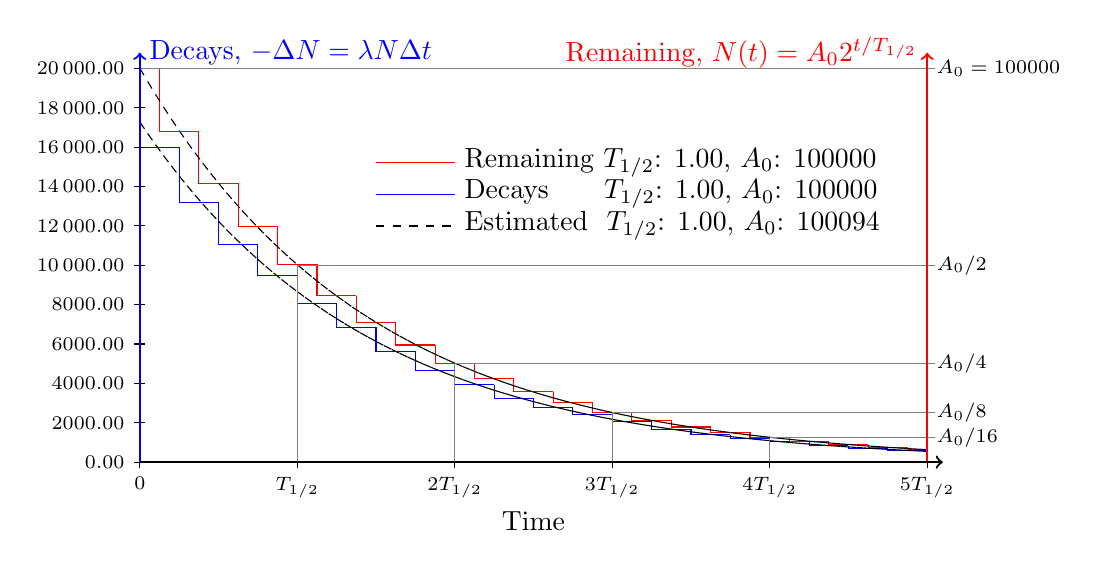
\begin{tikzpicture}
\begin{scope}[]
\clip (0,0) rectangle (10,5);
\begin{scope}[draw=blue]
\draw[] (0.0,3.99825) -- (0.5,3.99825);
\draw (0.5,3.99825) -- (0.5,3.29475) -- (1.0,3.29475);
\draw (1.0,3.29475) -- (1.0,2.769) -- (1.5,2.769);
\draw (1.5,2.769) -- (1.5,2.368) -- (2.0,2.368);
\draw (2.0,2.368) -- (2.0,2.011) -- (2.5,2.011);
\draw (2.5,2.011) -- (2.5,1.71425) -- (3.0,1.71425);
\draw (3.0,1.71425) -- (3.0,1.4085) -- (3.5,1.4085);
\draw (3.5,1.4085) -- (3.5,1.1675) -- (4.0,1.1675);
\draw (4.0,1.1675) -- (4.0,0.984) -- (4.5,0.984);
\draw (4.5,0.984) -- (4.5,0.813) -- (5.0,0.813);
\draw (5.0,0.813) -- (5.0,0.69425) -- (5.5,0.69425);
\draw (5.5,0.69425) -- (5.5,0.60925) -- (6.0,0.60925);
\draw (6.0,0.60925) -- (6.0,0.51625) -- (6.5,0.51625);
\draw (6.5,0.51625) -- (6.5,0.4195) -- (7.0,0.4195);
\draw (7.0,0.4195) -- (7.0,0.347) -- (7.5,0.347);
\draw (7.5,0.347) -- (7.5,0.29825) -- (8.0,0.29825);
\draw (8.0,0.29825) -- (8.0,0.2625) -- (8.5,0.2625);
\draw (8.5,0.2625) -- (8.5,0.2085) -- (9.0,0.2085);
\draw (9.0,0.2085) -- (9.0,0.17825) -- (9.5,0.17825);
\draw (9.5,0.17825) -- (9.5,0.149) -- (10.0,0.149);
\draw (10.0,0.149) -- (10.0,0.12175) -- (10.5,0.12175);
\draw (10.5,0.12175) -- (10.5,0.1085) -- (11.0,0.1085);
\draw (11.0,0.1085) -- (11.0,0.08825) -- (11.5,0.08825);
\draw (11.5,0.08825) -- (11.5,0.072) -- (12.0,0.072);
\draw (12.0,0.072) -- (12.0,0.06375) -- (12.5,0.06375);
\end{scope}
\begin{scope}[draw=red]
\draw[] (-0.25,5.0) -- (0.25,5.0);
\draw (0.25,5.0) -- (0.25,4.20035009765625) -- (0.75,4.20035009765625);
\draw (0.75,4.20035009765625) -- (0.75,3.541400146484375) -- (1.25,3.541400146484375);
\draw (1.25,3.541400146484375) -- (1.25,2.98760009765625) -- (1.75,2.98760009765625);
\draw (1.75,2.98760009765625) -- (1.75,2.514) -- (2.25,2.514);
\draw (2.25,2.514) -- (2.25,2.111800048828125) -- (2.75,2.111800048828125);
\draw (2.75,2.111800048828125) -- (2.75,1.7689500732421874) -- (3.25,1.7689500732421874);
\draw (3.25,1.7689500732421874) -- (3.25,1.48725) -- (3.75,1.48725);
\draw (3.75,1.48725) -- (3.75,1.25375) -- (4.25,1.25375);
\draw (4.25,1.25375) -- (4.25,1.0569500732421875) -- (4.75,1.0569500732421875);
\draw (4.75,1.0569500732421875) -- (4.75,0.8943500366210938) -- (5.25,0.8943500366210938);
\draw (5.25,0.8943500366210938) -- (5.25,0.7555) -- (5.75,0.7555);
\draw (5.75,0.7555) -- (5.75,0.6336500244140625) -- (6.25,0.6336500244140625);
\draw (6.25,0.6336500244140625) -- (6.25,0.5304000244140625) -- (6.75,0.5304000244140625);
\draw (6.75,0.5304000244140625) -- (6.75,0.4465) -- (7.25,0.4465);
\draw (7.25,0.4465) -- (7.25,0.37710000610351563) -- (7.75,0.37710000610351563);
\draw (7.75,0.37710000610351563) -- (7.75,0.31745001220703123) -- (8.25,0.31745001220703123);
\draw (8.25,0.31745001220703123) -- (8.25,0.26495001220703124) -- (8.75,0.26495001220703124);
\draw (8.75,0.26495001220703124) -- (8.75,0.22325) -- (9.25,0.22325);
\draw (9.25,0.22325) -- (9.25,0.18760000610351563) -- (9.75,0.18760000610351563);
\draw (9.75,0.18760000610351563) -- (9.75,0.15780000305175781) -- (10.25,0.15780000305175781);
\draw (10.25,0.15780000305175781) -- (10.25,0.1334499969482422) -- (10.75,0.1334499969482422);
\draw (10.75,0.1334499969482422) -- (10.75,0.11175) -- (11.25,0.11175);
\draw (11.25,0.11175) -- (11.25,0.0940999984741211) -- (11.75,0.0940999984741211);
\draw (11.75,0.0940999984741211) -- (11.75,0.07970000457763672) -- (12.25,0.07970000457763672);
\end{scope}
\begin{scope}[black,dashed]
\draw[] (0.0,4.320596879379904) -- (0.1,4.173944215473551);
\draw[] (0.1,4.173944215473551) -- (0.2,4.032269336912893);
\draw[] (0.2,4.032269336912893) -- (0.3,3.8954032842921604);
\draw[] (0.3,3.8954032842921604) -- (0.4,3.763182833141673);
\draw[] (0.4,3.763182833141673) -- (0.5,3.6354502992686935);
\draw[] (0.5,3.6354502992686935) -- (0.6,3.5120533507055547);
\draw[] (0.6,3.5120533507055547) -- (0.7,3.3928448260407587);
\draw[] (0.7,3.3928448260407587) -- (0.8,3.2776825589164122);
\draw[] (0.8,3.2776825589164122) -- (0.9,3.1664292084826937);
\draw[] (0.9,3.1664292084826937) -- (1.0,3.058952095607142);
\draw[] (1.0,3.058952095607142) -- (1.1,2.9551230446434493);
\draw[] (1.1,2.9551230446434493) -- (1.2,2.854818230571045);
\draw[] (1.2,2.854818230571045) -- (1.3,2.757918031323168);
\draw[] (1.3,2.757918031323168) -- (1.4,2.6643068851273326);
\draw[] (1.4,2.6643068851273326) -- (1.5,2.5738731526880225);
\draw[] (1.5,2.5738731526880225) -- (1.6,2.486508984047296);
\draw[] (1.6,2.486508984047296) -- (1.7,2.402110189964486);
\draw[] (1.7,2.402110189964486) -- (1.8,2.3205761176616226);
\draw[] (1.8,2.3205761176616226) -- (1.9,2.2418095307863894);
\draw[] (1.9,2.2418095307863894) -- (2.0,2.1657164934494597);
\draw[] (2.0,2.1657164934494597) -- (2.1,2.0922062581979195);
\draw[] (2.1,2.0922062581979195) -- (2.2,2.0211911577911668);
\draw[] (2.2,2.0211911577911668) -- (2.3,1.9525865006502348);
\draw[] (2.3,1.9525865006502348) -- (2.4,1.8863104698558417);
\draw[] (2.4,1.8863104698558417) -- (2.5,1.8222840255747204);
\draw[] (2.5,1.8222840255747204) -- (2.6,1.7604308107978583);
\draw[] (2.6,1.7604308107978583) -- (2.7,1.7006770602782357);
\draw[] (2.7,1.7006770602782357) -- (2.8,1.6429515125594625);
\draw[] (2.8,1.6429515125594625) -- (2.9,1.5871853249903976);
\draw[] (2.9,1.5871853249903976) -- (3.0,1.5333119916244022);
\draw[] (3.0,1.5333119916244022) -- (3.1,1.4812672639053133);
\draw[] (3.1,1.4812672639053133) -- (3.2,1.430989074045544);
\draw[] (3.2,1.430989074045544) -- (3.3,1.382417461004944);
\draw[] (3.3,1.382417461004944) -- (3.4,1.3354944989821302);
\draw[] (3.4,1.3354944989821302) -- (3.5,1.290164228333016);
\draw[] (3.5,1.290164228333016) -- (3.6,1.246372588834152);
\draw[] (3.6,1.246372588834152) -- (3.7,1.2040673552112877);
\draw[] (3.7,1.2040673552112877) -- (3.8,1.1631980748562656);
\draw[] (3.8,1.1631980748562656) -- (3.9,1.1237160076579724);
\draw[] (3.9,1.1237160076579724) -- (4.0,1.085574067875591);
\draw[] (4.0,1.085574067875591) -- (4.1,1.048726767984827);
\draw[] (4.1,1.048726767984827) -- (4.2,1.0131301644301465);
\draw[] (4.2,1.0131301644301465) -- (4.3,0.978741805218332);
\draw[] (4.3,0.978741805218332) -- (4.4,0.9455206792908462);
\draw[] (4.4,0.9455206792908462) -- (4.5,0.9134271676146429);
\draw[] (4.5,0.9134271676146429) -- (4.6,0.8824229959330795);
\draw[] (4.6,0.8824229959330795) -- (4.7,0.8524711891205949);
\draw[] (4.7,0.8524711891205949) -- (4.8,0.8235360270867108);
\draw[] (4.8,0.8235360270867108) -- (4.9,0.7955830021767695);
\draw[] (4.9,0.7955830021767695) -- (5.0,0.7685787780186059);
\draw[] (5.0,0.7685787780186059) -- (5.1,0.7424911497660728);
\draw[] (5.1,0.7424911497660728) -- (5.2,0.7172890056920083);
\draw[] (5.2,0.7172890056920083) -- (5.3,0.6929422900848423);
\draw[] (5.3,0.6929422900848423) -- (5.4,0.6694219674045888);
\draw[] (5.4,0.6694219674045888) -- (5.5,0.6466999876554843);
\draw[] (5.5,0.6466999876554843) -- (5.6,0.6247492529339674);
\draw[] (5.6,0.6247492529339674) -- (5.7,0.6035435851121131);
\draw[] (5.7,0.6035435851121131) -- (5.8,0.5830576946179774);
\draw[] (5.8,0.5830576946179774) -- (5.9,0.563267150275619);
\draw[] (5.9,0.563267150275619) -- (6.0,0.544148350168835);
\draw[] (6.0,0.544148350168835) -- (6.1,0.5256784934938564);
\draw[] (6.1,0.5256784934938564) -- (6.2,0.507835553367441);
\draw[] (6.2,0.507835553367441) -- (6.3,0.49059825055793194);
\draw[] (6.3,0.49059825055793194) -- (6.4,0.47394602810795333);
\draw[] (6.4,0.47394602810795333) -- (6.5,0.4578590268184828);
\draw[] (6.5,0.4578590268184828) -- (6.6,0.4423180615650576);
\draw[] (6.6,0.4423180615650576) -- (6.7,0.4273045984178732);
\draw[] (6.7,0.4273045984178732) -- (6.8,0.41280073253848826);
\draw[] (6.8,0.41280073253848826) -- (6.9,0.398789166826773);
\draw[] (6.9,0.398789166826773) -- (7.0,0.38525319129263924);
\draw[] (7.0,0.38525319129263924) -- (7.1,0.3721766631279479);
\draw[] (7.1,0.3721766631279479) -- (7.2,0.35954398745483007);
\draw[] (7.2,0.35954398745483007) -- (7.3,0.34734009872746274);
\draw[] (7.3,0.34734009872746274) -- (7.4,0.335550442765116);
\draw[] (7.4,0.335550442765116) -- (7.5,0.3241609593950491);
\draw[] (7.5,0.3241609593950491) -- (7.6,0.3131580656845519);
\draw[] (7.6,0.3131580656845519) -- (7.7,0.3025286397421364);
\draw[] (7.7,0.3025286397421364) -- (7.8,0.2922600050685593);
\draw[] (7.8,0.2922600050685593) -- (7.9,0.2823399154390125);
\draw[] (7.9,0.2823399154390125) -- (8.0,0.2727565402984537);
\draw[] (8.0,0.2727565402984537) -- (8.1,0.26349845065265703);
\draw[] (8.1,0.26349845065265703) -- (8.2,0.25455460543816094);
\draw[] (8.2,0.25455460543816094) -- (8.3,0.2459143383548557);
\draw[] (8.3,0.2459143383548557) -- (8.4,0.23756734514550923);
\draw[] (8.4,0.23756734514550923) -- (8.5,0.22950367130705826);
\draw[] (8.5,0.22950367130705826) -- (8.6,0.22171370021901302);
\draw[] (8.6,0.22171370021901302) -- (8.7,0.21418814167481504);
\draw[] (8.7,0.21418814167481504) -- (8.8,0.2069180208024712);
\draw[] (8.8,0.2069180208024712) -- (8.9,0.1998946673612523);
\draw[] (8.9,0.1998946673612523) -- (9.0,0.19310970540168873);
\draw[] (9.0,0.19310970540168873) -- (9.1,0.18655504327653508);
\draw[] (9.1,0.18655504327653508) -- (9.2,0.180222863990789);
\draw[] (9.2,0.180222863990789) -- (9.3,0.17410561587925602);
\draw[] (9.3,0.17410561587925602) -- (9.4,0.16819600360054385);
\draw[] (9.4,0.16819600360054385) -- (9.5,0.16248697943674306);
\draw[] (9.5,0.16248697943674306) -- (9.6,0.15697173488842153);
\draw[] (9.6,0.15697173488842153) -- (9.7,0.1516436925549066);
\draw[] (9.7,0.1516436925549066) -- (9.8,0.14649649829017228);
\draw[] (9.8,0.14649649829017228) -- (9.9,0.1415240136249772);
\draw[] (9.9,0.1415240136249772) -- (10.0,0.13672030844621477);
\end{scope}
\begin{scope}[black,dashed]
\draw[] (0.0,5.004728934357686) -- (0.1,4.834854990816327);
\draw[] (0.1,4.834854990816327) -- (0.2,4.670747025227576);
\draw[] (0.2,4.670747025227576) -- (0.3,4.512209324811377);
\draw[] (0.3,4.512209324811377) -- (0.4,4.359052819805141);
\draw[] (0.4,4.359052819805141) -- (0.5,4.211094857981897);
\draw[] (0.5,4.211094857981897) -- (0.6,4.068158986821887);
\draw[] (0.6,4.068158986821887) -- (0.7,3.9300747430778546);
\draw[] (0.7,3.9300747430778546) -- (0.8,3.796677449483049);
\draw[] (0.8,3.796677449483049) -- (0.9,3.6678080183595);
\draw[] (0.9,3.6678080183595) -- (1.0,3.543312761892366);
\draw[] (1.0,3.543312761892366) -- (1.1,3.4230432088440677);
\draw[] (1.1,3.4230432088440677) -- (1.2,3.3068559274896505);
\draw[] (1.2,3.3068559274896505) -- (1.3,3.1946123545621816);
\draw[] (1.3,3.1946123545621816) -- (1.4,3.0861786300042158);
\draw[] (1.4,3.0861786300042158) -- (1.5,2.9814254373282227);
\draw[] (1.5,2.9814254373282227) -- (1.6,2.880227849395627);
\draw[] (1.6,2.880227849395627) -- (1.7,2.7824651794305097);
\draw[] (1.7,2.7824651794305097) -- (1.8,2.6880208370903103);
\draw[] (1.8,2.6880208370903103) -- (1.9,2.5967821894218766);
\draw[] (1.9,2.5967821894218766) -- (2.0,2.508640426537035);
\draw[] (2.0,2.508640426537035) -- (2.1,2.4234904318474983);
\draw[] (2.1,2.4234904318474983) -- (2.2,2.341230656704347);
\draw[] (2.2,2.341230656704347) -- (2.3,2.2617629992925803);
\draw[] (2.3,2.2617629992925803) -- (2.4,2.1849926876363157);
\draw[] (2.4,2.1849926876363157) -- (2.5,2.1108281665751054);
\draw[] (2.5,2.1108281665751054) -- (2.6,2.039180988576581);
\draw[] (2.6,2.039180988576581) -- (2.7,1.9699657082552045);
\draw[] (2.7,1.9699657082552045) -- (2.8,1.9030997804713439);
\draw[] (2.8,1.9030997804713439) -- (2.9,1.8385034618891358);
\draw[] (2.9,1.8385034618891358) -- (3.0,1.7760997158757403);
\draw[] (3.0,1.7760997158757403) -- (3.1,1.715814120628568);
\draw[] (3.1,1.715814120628568) -- (3.2,1.6575747804209182);
\draw[] (3.2,1.6575747804209182) -- (3.3,1.601312239860179);
\draw[] (3.3,1.601312239860179) -- (3.4,1.546959401056331);
\draw[] (3.4,1.546959401056331) -- (3.5,1.494451443601979);
\draw[] (3.5,1.494451443601979) -- (3.6,1.4437257472684712);
\draw[] (3.6,1.4437257472684712) -- (3.7,1.3947218173259264);
\draw[] (3.7,1.3947218173259264) -- (3.8,1.3473812123980926);
\draw[] (3.8,1.3473812123980926) -- (3.9,1.301647474766011);
\draw[] (3.9,1.301647474766011) -- (4.0,1.2574660630373586);
\draw[] (4.0,1.2574660630373586) -- (4.1,1.2147842871011763);
\draw[] (4.1,1.2147842871011763) -- (4.2,1.173551245290403);
\draw[] (4.2,1.173551245290403) -- (4.3,1.1337177636772897);
\draw[] (4.3,1.1337177636772897) -- (4.4,1.0952363374292822);
\draw[] (4.4,1.0952363374292822) -- (4.5,1.0580610741554513);
\draw[] (4.5,1.0580610741554513) -- (4.6,1.0221476391758881);
\draw[] (4.6,1.0221476391758881) -- (4.7,0.9874532026488111);
\draw[] (4.7,0.9874532026488111) -- (4.8,0.9539363884923161);
\draw[] (4.8,0.9539363884923161) -- (4.9,0.9215572250398623);
\draw[] (4.9,0.9215572250398623) -- (5.0,0.8902770973706411);
\draw[] (5.0,0.8902770973706411) -- (5.1,0.8600587012579822);
\draw[] (5.1,0.8600587012579822) -- (5.2,0.8308659986808735);
\draw[] (5.2,0.8308659986808735) -- (5.3,0.8026641748455404);
\draw[] (5.3,0.8026641748455404) -- (5.4,0.7754195966658266);
\draw[] (5.4,0.7754195966658266) -- (5.5,0.7490997726528643);
\draw[] (5.5,0.7490997726528643) -- (5.6,0.7236733141661953);
\draw[] (5.6,0.7236733141661953) -- (5.7,0.6991098979801326);
\draw[] (5.7,0.6991098979801326) -- (5.8,0.6753802301207235);
\draw[] (5.8,0.6753802301207235) -- (5.9,0.6524560109301785);
\draw[] (5.9,0.6524560109301785) -- (6.0,0.6303099013171114);
\draw[] (6.0,0.6303099013171114) -- (6.1,0.6089154901523348);
\draw[] (6.1,0.6089154901523348) -- (6.2,0.5882472627713301);
\draw[] (6.2,0.5882472627713301) -- (6.3,0.5682805705458298);
\draw[] (6.3,0.5682805705458298) -- (6.4,0.5489916014882192);
\draw[] (6.4,0.5489916014882192) -- (6.5,0.5303573518537062);
\draw[] (6.5,0.5303573518537062) -- (6.6,0.5123555987063894);
\draw[] (6.6,0.5123555987063894) -- (6.7,0.49496487341650525);
\draw[] (6.7,0.49496487341650525) -- (6.8,0.4781644360572534);
\draw[] (6.8,0.4781644360572534) -- (6.9,0.4619342506706594);
\draw[] (6.9,0.4619342506706594) -- (7.0,0.44625496137298265);
\draw[] (7.0,0.44625496137298265) -- (7.1,0.43110786927116945);
\draw[] (7.1,0.43110786927116945) -- (7.2,0.41647491016282445);
\draw[] (7.2,0.41647491016282445) -- (7.3,0.40233863299310557);
\draw[] (7.3,0.40233863299310557) -- (7.4,0.3886821790428477);
\draw[] (7.4,0.3886821790428477) -- (7.5,0.3754892618231);
\draw[] (7.5,0.3754892618231) -- (7.6,0.36274414765209434);
\draw[] (7.6,0.36274414765209434) -- (7.7,0.35043163689148527);
\draw[] (7.7,0.35043163689148527) -- (7.8,0.33853704581948146);
\draw[] (7.8,0.33853704581948146) -- (7.9,0.3270461891192516);
\draw[] (7.9,0.3270461891192516) -- (8.0,0.31594536296172254);
\draw[] (8.0,0.31594536296172254) -- (8.1,0.30522132866258983);
\draw[] (8.1,0.30522132866258983) -- (8.2,0.2948612968940557);
\draw[] (8.2,0.2948612968940557) -- (8.3,0.2848529124324621);
\draw[] (8.3,0.2848529124324621) -- (8.4,0.27518423942363024);
\draw[] (8.4,0.27518423942363024) -- (8.5,0.26584374714833364);
\draw[] (8.5,0.26584374714833364) -- (8.6,0.2568202962709296);
\draw[] (8.6,0.2568202962709296) -- (8.7,0.24810312555474928);
\draw[] (8.7,0.24810312555474928) -- (8.8,0.23968183902840276);
\draw[] (8.8,0.23968183902840276) -- (8.9,0.2315463935876947);
\draw[] (8.9,0.2315463935876947) -- (9.0,0.2236870870183631);
\draw[] (9.0,0.2236870870183631) -- (9.1,0.21609454642535988);
\draw[] (9.1,0.21609454642535988) -- (9.2,0.20875971705487203);
\draw[] (9.2,0.20875971705487203) -- (9.3,0.20167385149575326);
\draw[] (9.3,0.20167385149575326) -- (9.4,0.19482849924748913);
\draw[] (9.4,0.19482849924748913) -- (9.5,0.18821549664225148);
\draw[] (9.5,0.18821549664225148) -- (9.6,0.18182695710902738);
\draw[] (9.6,0.18182695710902738) -- (9.7,0.17565526176820861);
\draw[] (9.7,0.17565526176820861) -- (9.8,0.16969305034542645);
\draw[] (9.8,0.16969305034542645) -- (9.9,0.1639332123937953);
\draw[] (9.9,0.1639332123937953) -- (10.0,0.15836887881409628);
\end{scope}
\draw[blue] (3.0,3.4) -- (4.0,3.4);
\node[right,] at (4.0,3.4) {Decays\ \ \ \ \ \ $T_{1/2}$:  1.00, $A_0$: 100000};
\draw[black,thick,dashed] (3.0,3.0) -- (4.0,3.0);
\node[right,] at (4.0,3.0) {Estimated \ $T_{1/2}$:  1.00, $A_0$: 100094};
\draw[red] (3.0,3.8) -- (4.0,3.8);
\node[right,] at (4.0,3.8) {Remaining $T_{1/2}$:  1.00, $A_0$: 100000};
\end{scope}
\draw (0,0cm + 2pt) -- (0, 0cm-2pt) node[below] {\scriptsize $0$};
\draw (2,0cm + 2pt) -- (2, 0cm-2pt) node[below] {\scriptsize $T_{1/2}$};
\draw (4,0cm + 2pt) -- (4, 0cm-2pt) node[below] {\scriptsize $2T_{1/2}$};
\draw (6,0cm + 2pt) -- (6, 0cm-2pt) node[below] {\scriptsize $3T_{1/2}$};
\draw (8,0cm + 2pt) -- (8, 0cm-2pt) node[below] {\scriptsize $4T_{1/2}$};
\draw (10,0cm + 2pt) -- (10, 0cm-2pt) node[below] {\scriptsize $5T_{1/2}$};
\draw (0cm + 2pt,0.    ) -- (0cm-2pt,0.    ) node[left] {\scriptsize{\num[round-mode=places,round-precision=2]{0}}};
\draw (0cm + 2pt,0.5    ) -- (0cm-2pt,0.5    ) node[left] {\scriptsize{\num[round-mode=places,round-precision=2]{2000}}};
\draw (0cm + 2pt,1.    ) -- (0cm-2pt,1.    ) node[left] {\scriptsize{\num[round-mode=places,round-precision=2]{4000}}};
\draw (0cm + 2pt,1.5    ) -- (0cm-2pt,1.5    ) node[left] {\scriptsize{\num[round-mode=places,round-precision=2]{6000}}};
\draw (0cm + 2pt,2.    ) -- (0cm-2pt,2.    ) node[left] {\scriptsize{\num[round-mode=places,round-precision=2]{8000}}};
\draw (0cm + 2pt,2.5    ) -- (0cm-2pt,2.5    ) node[left] {\scriptsize{\num[round-mode=places,round-precision=2]{10000}}};
\draw (0cm + 2pt,3.    ) -- (0cm-2pt,3.    ) node[left] {\scriptsize{\num[round-mode=places,round-precision=2]{12000}}};
\draw (0cm + 2pt,3.5    ) -- (0cm-2pt,3.5    ) node[left] {\scriptsize{\num[round-mode=places,round-precision=2]{14000}}};
\draw (0cm + 2pt,4.    ) -- (0cm-2pt,4.    ) node[left] {\scriptsize{\num[round-mode=places,round-precision=2]{16000}}};
\draw (0cm + 2pt,4.5    ) -- (0cm-2pt,4.5    ) node[left] {\scriptsize{\num[round-mode=places,round-precision=2]{18000}}};
\draw (0cm + 2pt,5.    ) -- (0cm-2pt,5.    ) node[left] {\scriptsize{\num[round-mode=places,round-precision=2]{20000}}};
\draw[thin,gray] (0.0,5.0) -- (10.1,5.0);
\node[right] at (10.0,5.0) {\scriptsize{$A_0 = 100000$}};
\draw[thin,gray] (2.0,2.5) -- (10.1,2.5);
\draw[thin,gray] (2.0,0.0) -- (2.0,2.5);
\node[right] at (10.0,2.5) {\scriptsize{$A_0/2$}};
\draw[thin,gray] (4.0,1.25) -- (10.1,1.25);
\draw[thin,gray] (4.0,0.0) -- (4.0,1.25);
\node[right] at (10.0,1.25) {\scriptsize{$A_0/4$}};
\draw[thin,gray] (6.0,0.625) -- (10.1,0.625);
\draw[thin,gray] (6.0,0.0) -- (6.0,0.625);
\node[right] at (10.0,0.625) {\scriptsize{$A_0/8$}};
\draw[thin,gray] (8.0,0.3125) -- (10.1,0.3125);
\draw[thin,gray] (8.0,0.0) -- (8.0,0.3125);
\node[right] at (10.0,0.3125) {\scriptsize{$A_0/16$}};
\node[right,blue] at (0.0,5.2) {Decays, $-\Delta N = \lambda N \Delta t$};
\node[left,red] at (10.0,5.2) {Remaining, $N(t) = A_0 2^{t/T_{1/2}}$};
\node[below] at (5.0,-0.5) {Time};
\draw[blue,thick,->] (0.0,0.0) -- (0.0,5.2);
\draw[red,thick,->] (10.0,0.0) -- (10.0,5.2);
\draw[thick,->] (0.0,0.0) -- (10.2,0.0);
\end{tikzpicture}
%%% Local Variables: 
%%% mode: latex 
%%% TeX-master: "master" 
%%% End:


  \caption{ Attempt to show two different axes in plot. }
\end{figure}
 
\end{document}


  
%%% Local Variables: 
%%% mode: latex
%%% TeX-master: t
%%% End: 
